% Questo file definisce lo stile che verrà applicato
% ad ogni pagina di contenuto
\documentclass[a4paper,11pt]{article}

\usepackage{ifthen}
\usepackage[
 a4paper,
 top=2.5cm,
 bottom=2.5cm,
 left=1.5cm,
 right=1.5cm,
 head=30pt
]{geometry}
\usepackage[italian]{babel}
\usepackage[utf8x]{inputenc}
\usepackage[T1]{fontenc}
\usepackage{fancyhdr}
\usepackage[colorlinks=true, urlcolor=black, citecolor=black, linkcolor=black]{hyperref}
\usepackage{tabularx}
\usepackage{multirow}
\usepackage{booktabs}
\usepackage{color}
\usepackage[dvipsnames]{xcolor}
\usepackage{graphicx}
\usepackage{eurosym}
\usepackage{amsmath}
\usepackage{relsize}
\usepackage{placeins}
\usepackage{ltablex}
\usepackage{float}

\usepackage[multidot]{grffile}
\usepackage{xcolor,colortbl}
\definecolor{lightblue}{HTML}{56B4E6}
\definecolor{blue}{HTML}{2953A1}
\definecolor{darkblue}{HTML}{1E396E}
\usepackage{longtable}

\usepackage[toc,page]{appendix}
\renewcommand\appendixtocname{Appendice}
\renewcommand{\appendixpagename}{Appendice}

\newcommand\pagenumberingnoreset[1]{\gdef\thepage{\csname @#1\endcsname\c@page}}

% Cambia il font 
\renewcommand*\rmdefault{qhv}

% ***STILE PAGINA***
\pagestyle{fancy}
\fancyhf{}
\setlength{\headheight}{1cm} 
% No indentazione paragrafo
\setlength{\parindent}{0pt}

% ***INTESTAZIONE***
\newcommand\textline[4][t]{%
  \noindent\parbox[#1]{.333\textwidth}{\raisebox{-0.40\height}{#2}}%
  \parbox[#1]{.333\textwidth}{\centering #3}%
  \parbox[#1]{.333\textwidth}{\raggedleft #4}%
}

\lhead{
	\textline[t]{
\includegraphics[width=1cm, keepaspectratio=true]{../../../Template/Logo/Logo.png}}{\progettoShort}{\documento}
}

\renewcommand{\headrulewidth}{0.4pt}  %Linea sotto l'intestazione

% ***PIÈ DI PAGINA***
\lfoot{\textit{\gruppoLink}\\ \footnotesize{\email}}
\rfoot{\thepage} %per le prime pagine: mostra solo il numero romano
\cfoot{}
\renewcommand{\footrulewidth}{0.4pt}   %Linea sopra il piè di pagina


% Ridefinisce command \paragraph{} andando a capo ogni dopo la parola dentro le parentesi ed ha la possibiltà di enumerazione fino a n cifre modificando il numero dentro "secnumdepth"
\usepackage{titlesec}

\setcounter{secnumdepth}{7}
\setcounter{tocdepth}{7}


% Visualizza paragraph come una section
\titleformat{\paragraph}{\normalfont\normalsize\bfseries}{\theparagraph}{1em}{}
\titlespacing*{\paragraph}{0pt}{3.25ex plus 1ex minus .2ex}{1.5ex plus .2ex}

\titleformat{\subparagraph}{\normalfont\normalsize\bfseries}{\thesubparagraph}{1em}{}
\titlespacing*{\subparagraph}{0pt}{3.25ex plus 1ex minus .2ex}{1.5ex plus .2ex}

\makeatletter
\newcounter{subsubparagraph}[subparagraph]
\renewcommand\thesubsubparagraph{%
  \thesubparagraph.\@arabic\c@subsubparagraph}
\newcommand\subsubparagraph{%
  \@startsection{subsubparagraph}    % counter
    {6}                              % level
    {\parindent}                     % indent
    {3.25ex \@plus 1ex \@minus .2ex} % beforeskip
    {0.75em}                           % afterskip
    {\normalfont\normalsize\bfseries}}
\newcommand\l@subsubparagraph{\@dottedtocline{6}{13em}{5.5em}} %gestione dell'indice
\newcommand{\subsubparagraphmark}[1]{}
\makeatother

\makeatletter
\newcounter{subsubsubparagraph}[subsubparagraph]
\renewcommand\thesubsubsubparagraph{%
  \thesubsubparagraph.\@arabic\c@subsubsubparagraph}
\newcommand\subsubsubparagraph{%
  \@startsection{subsubsubparagraph}    % counter
    {7}                              % level
    {\parindent}                     % indent
    {3.25ex \@plus 1ex \@minus .2ex} % beforeskip
    {0.75em}                           % afterskip
    {\normalfont\normalsize\bfseries}}
\newcommand\l@subsubsubparagraph{\@dottedtocline{7}{16em}{6.5em}} %gestione dell'indice
\newcommand{\subsubsubparagraphmark}[1]{}
\makeatother

%Generali
\newcommand{\capitolato}{C5 - Monolith: An interactive bubble provider}
\newcommand{\progettoShort}{Monolith}
\newcommand{\progetto}{Monolith: An interactive bubble provider}
\newcommand{\gruppo}{NPE Developers}
\newcommand{\gruppoLink}{\href{https://gitlab.com/npe-developers}{NpeDevelopers}}
\newcommand{\email}{\href{mailto:npe.developers@gmail.com}{\textcolor{blue}{npe.developers@gmail.com}}}
\newcommand{\password}{NP3Devel0pers}
\newcommand{\myincludegraphics}[2][]{%
	\setbox0=\hbox{\phantom{X}}%
	\vtop{
		\hbox{\phantom{X}}
		\vskip-\ht0
		\hbox{\includegraphics[#1]{#2}}}
}




%Componenti del gruppo
\newcommand{\RM}{Riccardo Montagnin}
\newcommand{\MT}{Manuel Turetta}
\newcommand{\FB}{Francesco Bazzerla}
\newcommand{\SL}{Stefano Lia}
\newcommand{\LD}{Luca Dario}
\newcommand{\DC}{Diego Cavestro}
\newcommand{\ND}{Nicolò Dovico}

%Ruoli
\newcommand{\Pm}{Project Manager}
\newcommand{\Am}{Amministratore}
\newcommand{\AmP}{Amministratori}
\newcommand{\An}{Analista}
\newcommand{\AnP}{Analisti}
\newcommand{\Dev}{Sviluppatore}
\newcommand{\DevP}{Sviluppatori}
\newcommand{\Ver}{Verificatore}
\newcommand{\VerP}{Verificatori}
\newcommand{\Progr}{Programmatore}
\newcommand{\ProgrP}{Programmatori}
\newcommand{\Prog}{Progettista}
\newcommand{\ProgP}{Progettisti}



%Firme
\newcommand{\RMFirma}{\myincludegraphics[scale = 0.5]{../../../Template/Firme/RM.png}}
\newcommand{\MTFirma}{\myincludegraphics[scale = 0.5]{../../../Template/Firme/MT.png}}
\newcommand{\FBFirma}{\myincludegraphics[scale = 0.5]{../../../Template/Firme/FB.png}}
\newcommand{\SLFirma}{\myincludegraphics[scale = 0.5]{../../../Template/Firme/SL.png}}
\newcommand{\LDFirma}{\myincludegraphics[scale = 0.5]{../../../Template/Firme/LD.png}}
\newcommand{\DCFirma}{\myincludegraphics[scale = 0.5]{../../../Template/Firme/DC.png}}
\newcommand{\NDFirma}{\myincludegraphics[scale = 0.5]{../../../Template/Firme/ND.png}}

%Professori e proponente
\newcommand{\TV}{Prof. Tullio Vardanega}
\newcommand{\RC}{Prof. Riccardo Cardin}
\newcommand{\RB}{Red Babel}
\newcommand{\proponente}{Red Babel}

%Documenti
\newcommand{\Gl}{Glossario}
\newcommand{\glossario}{\textit{\Gl\_v.2.0.0.pdf}}
\newcommand{\AdR}{Analisi dei Requisiti}
\newcommand{\analisiDeiRequisiti}{\textit{\AdR\_v.2.0.0.pdf}}
\newcommand{\AdRvDue}{AnalisiDeiRequisiti}
\newcommand{\NdP}{Norme di Progetto}
\newcommand{\normeDiProgetto}{\textit{\NdP\_v.2.0.0.pdf}}
\newcommand{\PdP}{Piano di Progetto}
\newcommand{\pianoDiProgetto}{\textit{\PdP\_v.2.0.0.pdf}}
\newcommand{\SdF}{Studio di Fattibilità}
\newcommand{\studioDiFattibilita}{\textit{\SdF\_v.2.0.0.pdf}}
\newcommand{\PdQ}{Piano di Qualifica}
\newcommand{\pianoDiQualifica}{\textit{\PdQ\_v.2.0.0.pdf}}
\newcommand{\VI}{Verbale Interno}
\newcommand{\VE}{Verbale Esterno}
\newcommand{\ST}{Specifica Tecnica}
\newcommand{\MU}{Manuale Utente}
\newcommand{\DDP}{Definizione di Prodotto}

%Periodo di progetto
\newcommand{\ARM}{Analisi dei Requisiti di Massima}
\newcommand{\ARD}{Analisi dei Requisiti in Dettaglio}
\newcommand{\PA}{Progettazione Architetturale}
\newcommand{\PD}{Progettazione di Dettaglio}
\newcommand{\COD}{Codifica}
\newcommand{\VV}{Verifica e Testing Finale}

%Consegne
\newcommand{\RR}{Revisione dei Requisiti}
\newcommand{\RP}{Revisione di Progettazione}
\newcommand{\RQ}{Revisione di Qualifica}
\newcommand{\RA}{Revisione di Accettazione}


%Formattazione
\newcommand{\termine}[1]{\textit{#1}\small{$_G$}}
\newcommand{\link}[1]{\href{#1}{\textcolor{blue}{\texttt{#1}}}} 

% Testi ricorrenti
\newcommand{\scopoProdotto}{L'obiettivo di questo progetto è la realizzazione di un \termine{SDK} che permetta la creazione di bolle interattive, le quali, successivamente, verranno utilizzate all'interno dell'applicazione di messaggistica istantanea open source \termine{Rocket.chat}. \\
Dopo la realizzazione di tale \termine{SDK}, è proposto lo sviluppo di un'applicazione in grado di sfruttare l'\termine{SDK} per implementare un uso originale. L'applicazione scelta dal \termine{team} consiste nella bolla lista-spesa e nei suoi vari utilizzi all'interno della piattaforma \termine{Rocket.chat}.
}
\newcommand{\descrizioneGlossario}{Al fine di mantenere questo documento compatto e di facile lettura è stato realizzato un glossario esterno contenente tutte le definizioni dei termini che più comunemente verranno presentati al lettore.  
Tale glossario si ritrova all'interno del file \glossario, e contiene tutti e soli i termini che vengono marcati con una \textit{G} a pedice.
}
\newcommand{\riferimentiNormativi}{
	\begin{itemize}
		\item \textbf{Norme di Progetto}: \normeDiProgetto
		\item \textbf{\termine{Capitolato} d'appalto C5: Monolith - An Interactive bubble provider} \\
			  \link{http://www.math.unipd.it/~tullio/IS-1/2016/Progetto/C5.pdf}
	\end{itemize}
}

% Comandi per generare l'intro
\newcommand{\documento}{\DDP}
\newcommand{\versione}{0.2.0}
\newcommand{\redatori}{\DC\\ & \LD\\ & \FB\\ & \ND\\ & \SL\\}
\newcommand{\revisori}{\RM}
\newcommand{\dataApprovazione}{6 marzo 2017}
\newcommand{\approvazione}{\MT}
\newcommand{\statoapprovazione}{Approvato}
\newcommand{\uso}{Esterno}
\newcommand{\destinatari}{\RB\\ & \TV\\ & \RC}

\newcommand{\sommario}{Questo documento descrive l'\termine{architettura di dettaglio} di \capitolato.}

\newcommand{\modifiche}{
3.0.0 & Approvazione del documento - Creare nuova versione del documento & \SL & \Pm & 07/05/2017 \\\midrule
2.1.0 & Verifica documento - Correzione errori & \LD & \Ver & 04/05/2017 \\\midrule
2.0.4 & Aggiunta la nota riguardante la forma del \MU\ di \progettoShort\ - In seguito a quanto deciso in data 03 maggio 2017 e riportato nell'apposito verbale & \ND & \Am & 04/05/2017 \\\midrule
	2.0.3 & Modificata la sezione delle metriche per la codifica - Aggiungere regole più precise per facilitare la stesura del codice & \ND & \Am & 28/03/2017 \\\midrule
2.0.2 & Aggiunte sezioni mancanti - Migliorare la profondità del documento come segnalato nella correzione in seguito alla \RP & \SL & \Am & 27/03/2017 \\
\midrule
2.0.1 & Riorganizzata la sezione degli strumenti - Aggiungere chiarezza su quale strumento sia usato per quale attività & \SL & \Am & 26/03/2017 \\
\midrule
2.0.0 & Approvazione del documento - Creare nuova versione del documento & \DC & \Pm & 04/03/2017 \\
\midrule 
1.1.0 & Verifica del documento - Correzioni errori & \LD & \Ver & 04/03/2017 \\
\midrule 
	1.0.2 & Aggiunta metriche - Aggiunta profondità come segnalato nella correzione in seguito alla \RR & \ND & \Am & 28/02/2017 \\
	\midrule
	1.0.1 & Aggiornamenti sezioni 3 e 4 - Aggiunta ampiezza come segnalato nella correzione in seguito alla \RR & \ND & \Am & 27/02/2017 \\
	\midrule
	1.0.0 & Approvazione - Creare la prima versione del documento & \SL & \Pm & 04/01/2016 \\
	\midrule
	0.4.0 & Verifica sottosezione 4.4 - Correzione errori & \RM & \Ver & 29/12/2016 \\\midrule
	0.3.1 & Stesura sottosezione 4.4 - Aggiunte norme sul processo di formazione & \DC & \Ver & 29/12/2016 \\\midrule
	0.3.0 & Verifica sezione 4 - Correzione errori & \RM &\Ver & 27/12/2016 \\\midrule
	0.2.0 & Verifica sezione 3 - Correzione errori & \RM & \Ver & 24/12/2016 \\\midrule
	0.1.0  & Verifica sezioni 1 e 2 - Correzioni errori & \RM & \Ver & 23/12/2016\\\midrule
    0.0.5 & Stesura sezione 4 - stabilire norme per il coordinamento e pianificazione & \DC & \Am & 21/12/2016 \\\midrule
    0.0.4 & Stesura sezione 2 - Definizione dei processi primari per il progetto & \LD & \Am & 20/12/2017 \\\midrule
    0.0.3 & Stesura sezione 1 e modifica del template - Introduzione al documento & \FB & \Am & 18/12/2016 \\\midrule
    0.0.2 & Stesura sezione 3 - Definizione dei processi di supporto  & \ND & \Am & 17/12/2016 \\\midrule
    0.0.1 & Creazione del template - Inizio documento & \SL & \Am & 15/12/2016 \\\midrule
}


\begin{document}

% Questo file contiene il layout della prima pagina
\pagenumbering{gobble}

\title{
\includegraphics[width=8cm, keepaspectratio=true]{../../../Template/Logo/Logo.png} \\
	\documento \\
	Versione \versione
}
\date{\dataApprovazione}

\maketitle

\begin{center}

\begin{tabular}{ r | l }
  \textbf{Ruolo} & \textbf{Componente} \\
  Redazione & \redatori \\
  Revisione & \revisori \\
  Approvazione & \approvazione \\
  \\
  Stato & \statoapprovazione \\
  Uso & \uso \\
  Destinatari & \destinatari
\end{tabular}
\end{center}

\begin{center}
\textbf{Sommario\\}
\sommario \\
\vspace{1.5cm}\email
\end{center}

\clearpage

\pagenumbering{arabic}
%Questo file si occupa di generare la tabella delle modifiche
\pagenumbering{Roman}

\begin{center}
    \Large{\textbf{Registro delle modifiche}}
    	\\\vspace{0.5cm}
    	\normalsize
    \begin{tabularx}{\textwidth}{cXXcc}
        \textbf{Versione} & \textbf{Modifica - Motivazione} & \textbf{Autore} & \textbf{Ruolo} & \textbf{Data} \\\toprule
        \modifiche
    \end{tabularx}
\end{center}

\newpage



\tableofcontents

\newpage

\setcounter{table}{0}
\listoftables

\newpage

\listoffigures

\newpage

\pagenumbering{arabic}


\section{Introduzione}
\subsection{Scopo del documento}
Questo documento vuole definire le strategie che il \termine{team} ha deciso di adottare per perseguire gli obiettivi di qualità di processo e di prodotto ricercati. A tal fine è necessaria una costante attività di verifica e validazione del lavoro svolto in modo da poter rilevare e correggere le anomalie che potrebbero nascere.

\subsection{Scopo del prodotto}
\scopoProdotto

\subsection{Glossario}
\descrizioneGlossario

\subsection{Riferimenti}
\subsubsection{Normativi}
\riferimentiNormativi

\subsubsection{Informativi}
\begin{itemize}
	\item \textbf{\AdR}: \analisiDeiRequisiti;
	\item \textbf{\PdP}: \pianoDiProgetto;
	\item \textbf{\textit{Slide} dell'insegnamento di Ingegneria del Software}: \\
		  \link{http://www.math.unipd.it/~tullio/IS-1/2016/}
	\item \textbf{\textit{Standard} ISO/IEC 9126}: Product quality \\
	 	  \link{https://en.wikipedia.org/wiki/ISO/IEC\_9126}
	\item \textbf{\textit{Standard} tecnici ISO/IEC 15504}: Software process assessment \\
		  \link{https://en.wikipedia.org/wiki/ISO/IEC\_15504}
	\item \textbf{Ciclo di Deming (\termine{PDCA})}: Miglioramento dei processi \\
		  \link{https://en.wikipedia.org/wiki/PDCA}
\end{itemize}

\newpage
\newpage
\section{Standard di Progetto}
\subsection{Documentazione del codice}
Gli standard per la scrittura della documentazione del codice sono definiti nelle \normeDiProgetto.

\subsection{Denominazione entità e relazioni}
Tutti gli elementi definiti, siano essi package, classi, metodi o attributi, devono avere denominazioni chiare ed autoesplicative. \\
Nel caso in cui il nome risulti essere lungo è preferibile anteporre la chiarezza alla lunghezza.
Sono ammesse abbreviazioni se:
\begin{itemize}
	\item immediatamente comprensibili;
	\item non ambigue;
	\item sufficientemente contestualizzate.
\end{itemize}
Le regole tipografiche relativi ai nomi delle entità sono definiti nelle \normeDiProgetto.

\subsection{Codifica}
Gli standard di programmazione sono definiti e descritti nelle  \normeDiProgetto.

\subsection{Strumenti di lavoro}
Gli strumenti da adottare e le procedure da seguire per utilizzarli correttamente durante la realizzazione del prodotto software sono definiti nelle  \normeDiProgetto.
\newpage
\newpage
\section{Architettura}

\subsection{Metodo e Formalismo}
Nell’esposizione dell’architettura dell’applicazione si procederà con un approccio \termine{top-down} descrivendo l’architettura dal generale al particolare. Si procederà quindi alla descrizione dei
\termine{packages} e dei componenti, per poi descrivere nel dettaglio le singole classi, specificando per
ognuna il tipo, l’obiettivo, la funzione, relazioni in ingresso e uscita e i metodi e attributi contenuti. Successivamente si procederà ad elencare i diagrammi di sequenza che descriveranno il funzionamento dell'\termine{SDK} e dell'applicazione. 


\subsection{Informazioni Generali}
Il principio di progettazione che abbiamo addottato è il Common Closure Principale per i seguenti motivi:
\begin{itemize}
\item Suddivisione più logica dei vari package e classi.
\item Aumenta la manutenibilità del codice nel tempo.
\end{itemize}

%\begin{figure}[H]
%	\centering
%	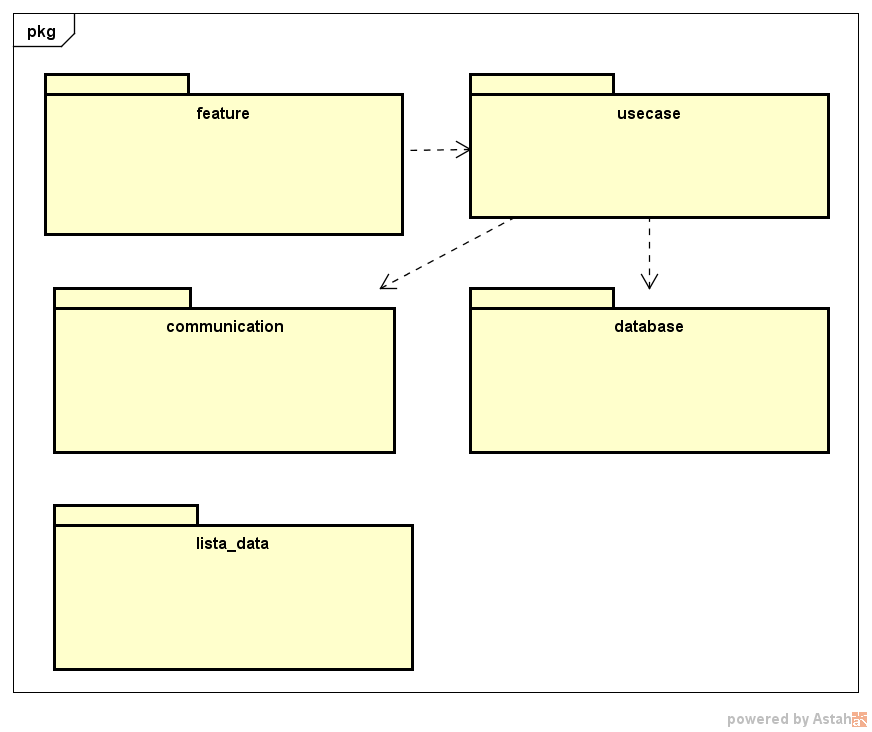
\includegraphics[scale=0.5]{Sezioni/Packages/App/application.png}
%	\caption{Package application}
%\end{figure}


\subsection{SDK}

\subsubsection{Creazione di un widget immagine}

\label{Creazione di un widget immagine}
\begin{figure}[ht]
	\centering
	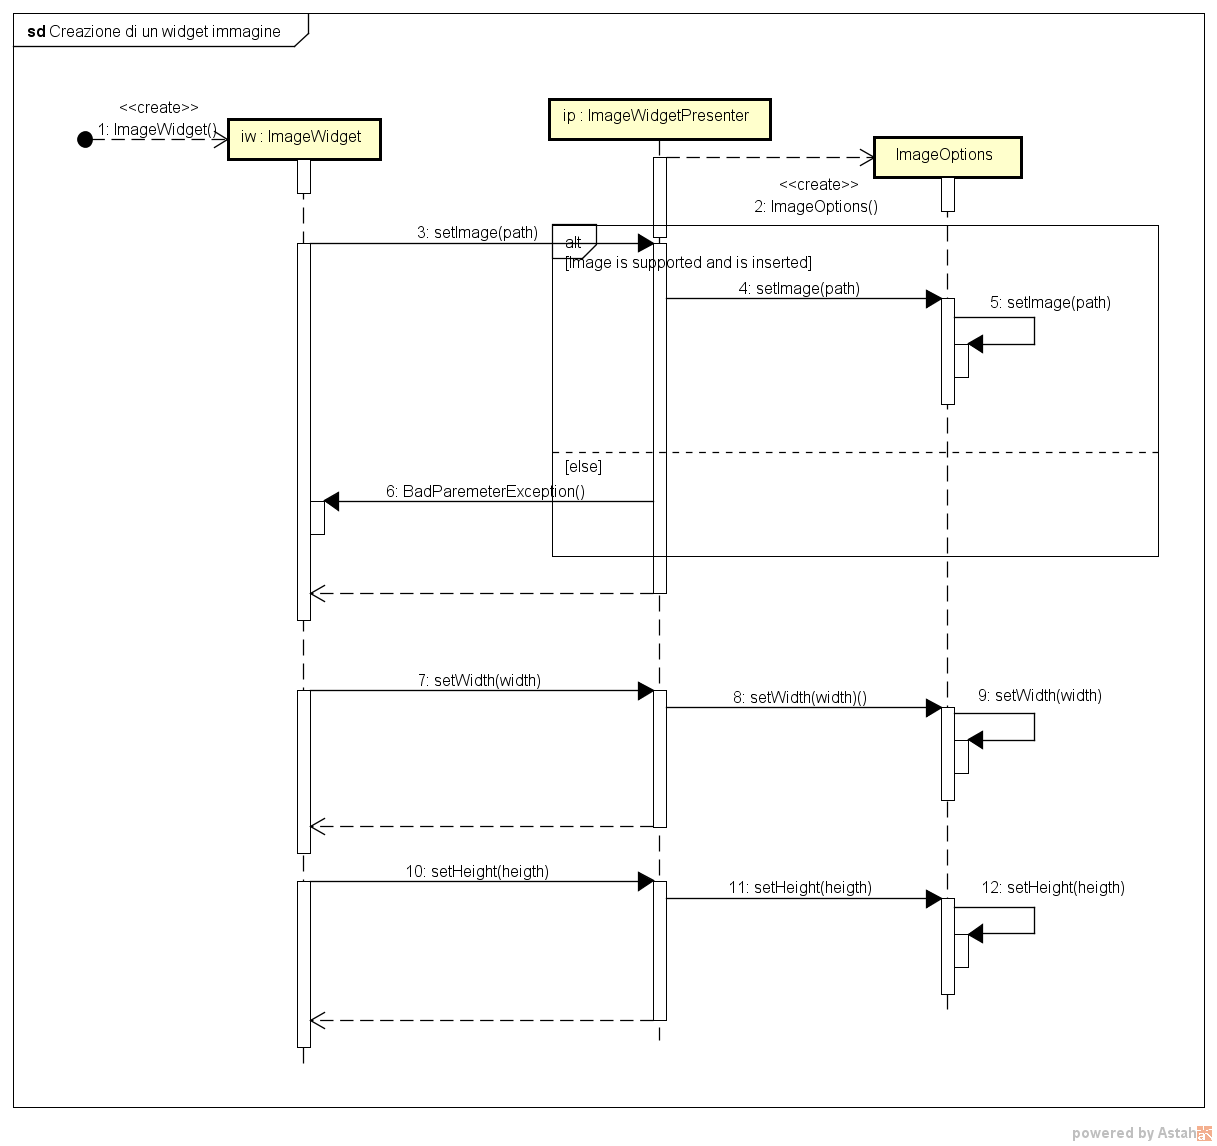
\includegraphics[width=16cm, height=14cm]{Sezioni/Diagrammi/img/Creazione di un widget immagine.png}
	\caption{Creazione di un widget immagine}
\end{figure}

Lo sviluppatore può creare un widget di tipo immagine per aggiungerlo ad una sua ipotetica \termine{bolla}. Durante la costruzione, come si vede dallo schema, vengono invocati tre metodi. Il primo per impostare l'immagine e gli altri due per impostare rispettivamente la larghezza ed altezza di essa. Il tipo delle immagini supportate sono le stesse supportate da \termine{Rocket.Chat} ovvero:
\begin{itemize}
\item .jpeg
\item .gif
\item .png
\item .jpg
\end{itemize}
Se l'immagine inserita non appartiene ad uno di questi formati oppure non viene inserita dallo sviluppatore il metodo \texttt{setText} di \texttt{TextWidgetPresenter} lancerà un'eccezione di tipo \texttt{BadParameterException}. \\
Le frecce di ritorno dall'\texttt{ImageWidgetPresenter} all'\texttt{ImageWidget} sono state inserite poiché il cambiamento dei dati sul \termine{Presenter} ha effetto anche sulla View. La comunicazione tra queste due unità avviene tramite il \termine{framework} \termine{vue.js}. \\
Si noti, infine, che i metodi invocati da \texttt{ImageWidget} vengono chiamati in quest'ordine dal suo costruttore senza parametri. Tali metodi possono anche essere chiamati singolarmente dallo sviluppatore secondo l'ordine che egli preferisce. Queste azioni non verranno ulteriormente descritte poiché ritenute ridondanti.

\newpage

\subsubsection{Creazione di un widget di testo}

\label{Creazione di un widget di testo}
\begin{figure}[H]
	\centering
	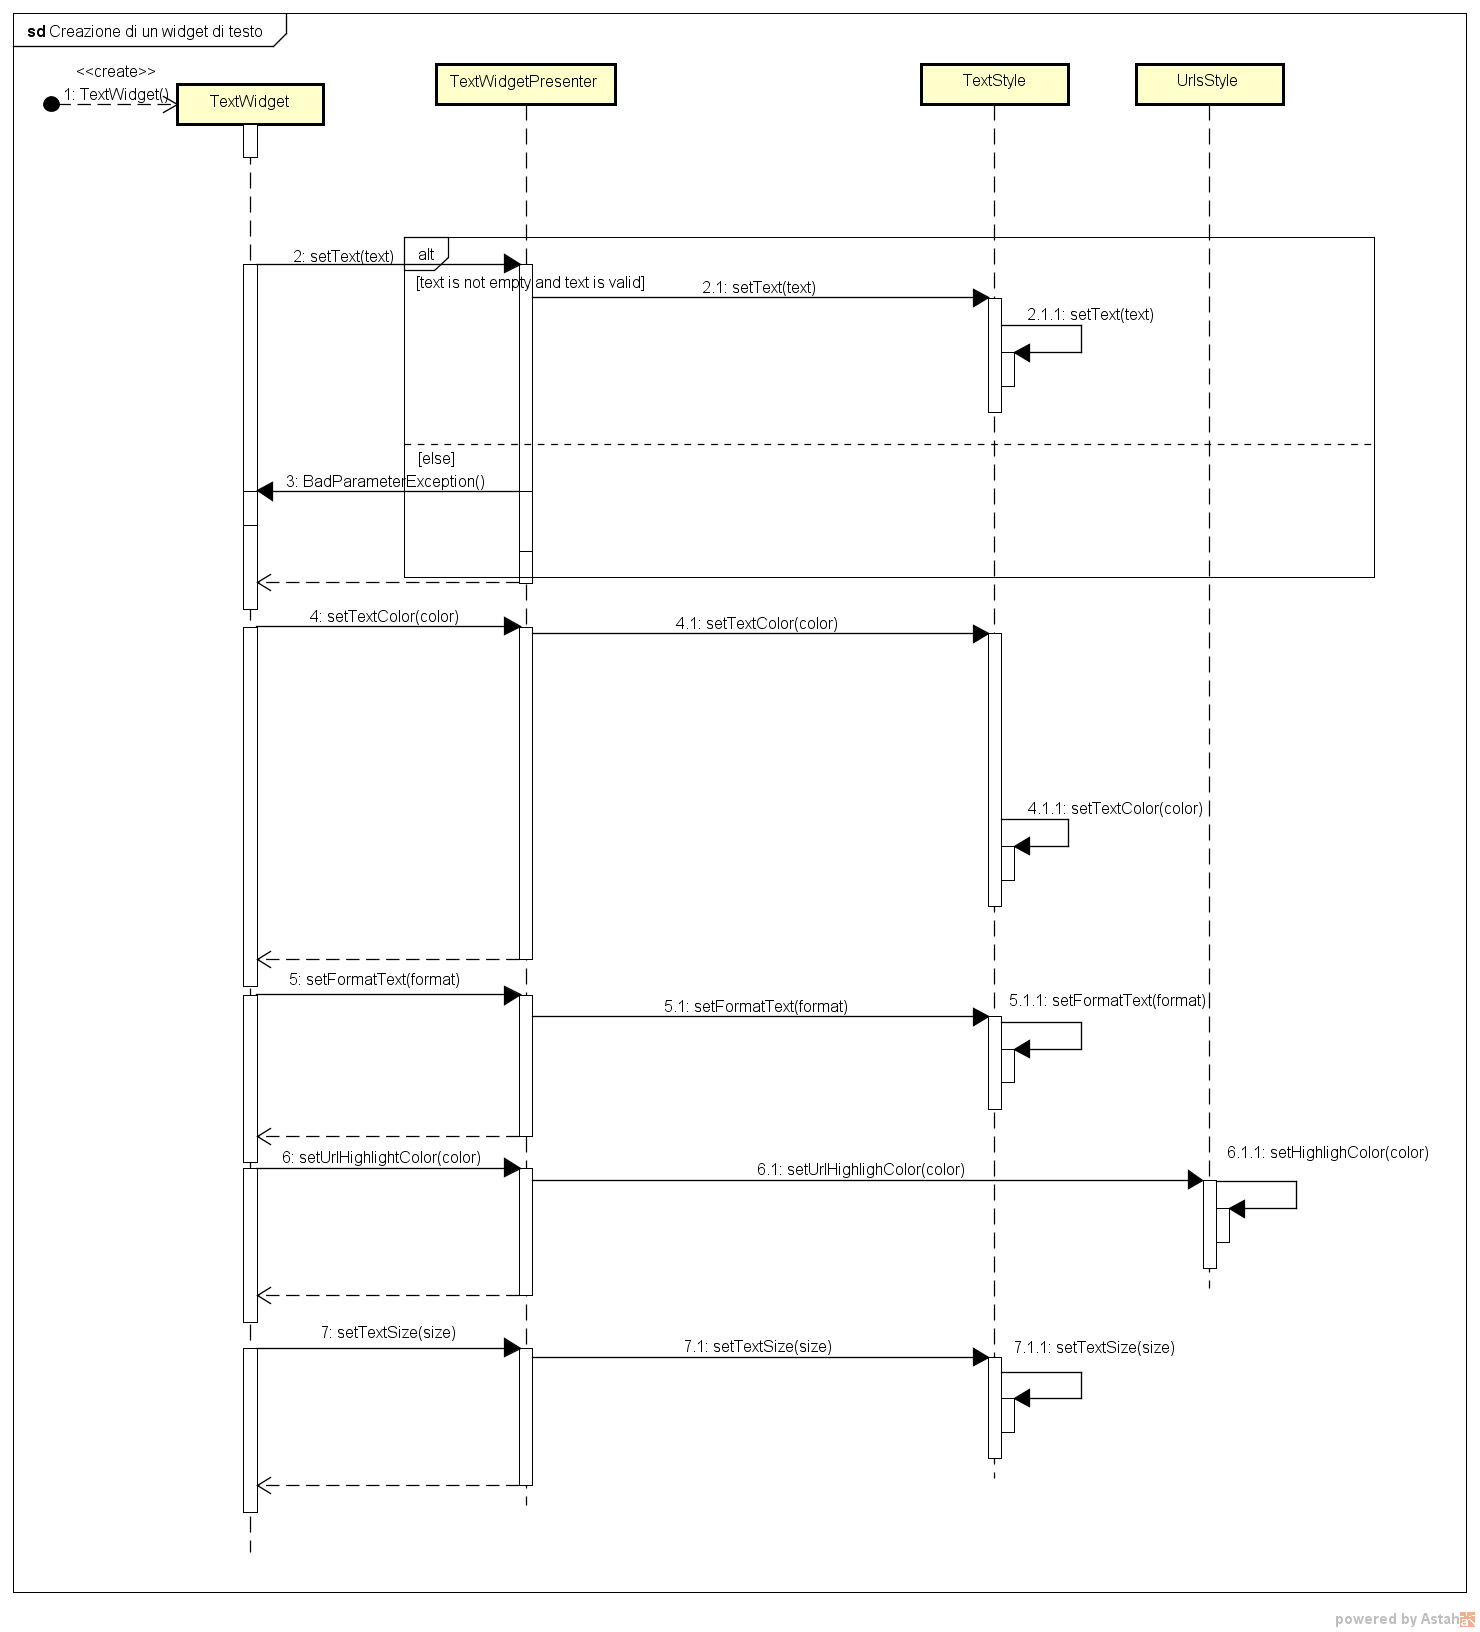
\includegraphics[width=16cm, height=14cm]{Sezioni/Diagrammi/img/Creazione di un widget di testo.png}
	\caption{Creazione di un widget di testo}
\end{figure}

Lo sviluppatore può creare un widget di tipo testo per aggiungerlo ad una sua ipotetica \termine{bolla}. Affinché non si verifichino errori il testo inserito nel widget deve essere valido, ovvero non deve contenere caratteri speciali se non quelli supportati dal tipo di codifica UTF-8 e non deve essere del testo vuoto. Se ciò dovesse capitare il metodo \texttt{setText} di \texttt{TextWidgetPresenter} lancerà un'eccezione di tipo \texttt{BadParameterException}. \\
Le frecce di ritorno dal \texttt{TextWidgetPresenter}  al \texttt{TextWidget} sono state inserite poiché il cambiamento dei dati sul \termine{Presenter} ha effetto anche sulla View. La comunicazione tra queste due unità avviene tramite il \termine{framework} \termine{vue.js}. \\
Si noti, infine, che i metodi invocati da \texttt{TextWidget} vengono chiamati in quest'ordine dal suo costruttore senza parametri. Tali metodi possono anche essere chiamati singolarmente dallo sviluppatore secondo l'ordine che egli preferisce. Queste azioni non verranno ulteriormente descritte poiché ritenute ridondanti.

\newpage

\subsubsection{Creazione di un widget Checklist}

\label{Creazione di un widget Checklist}
\begin{figure}[H]
	\centering
	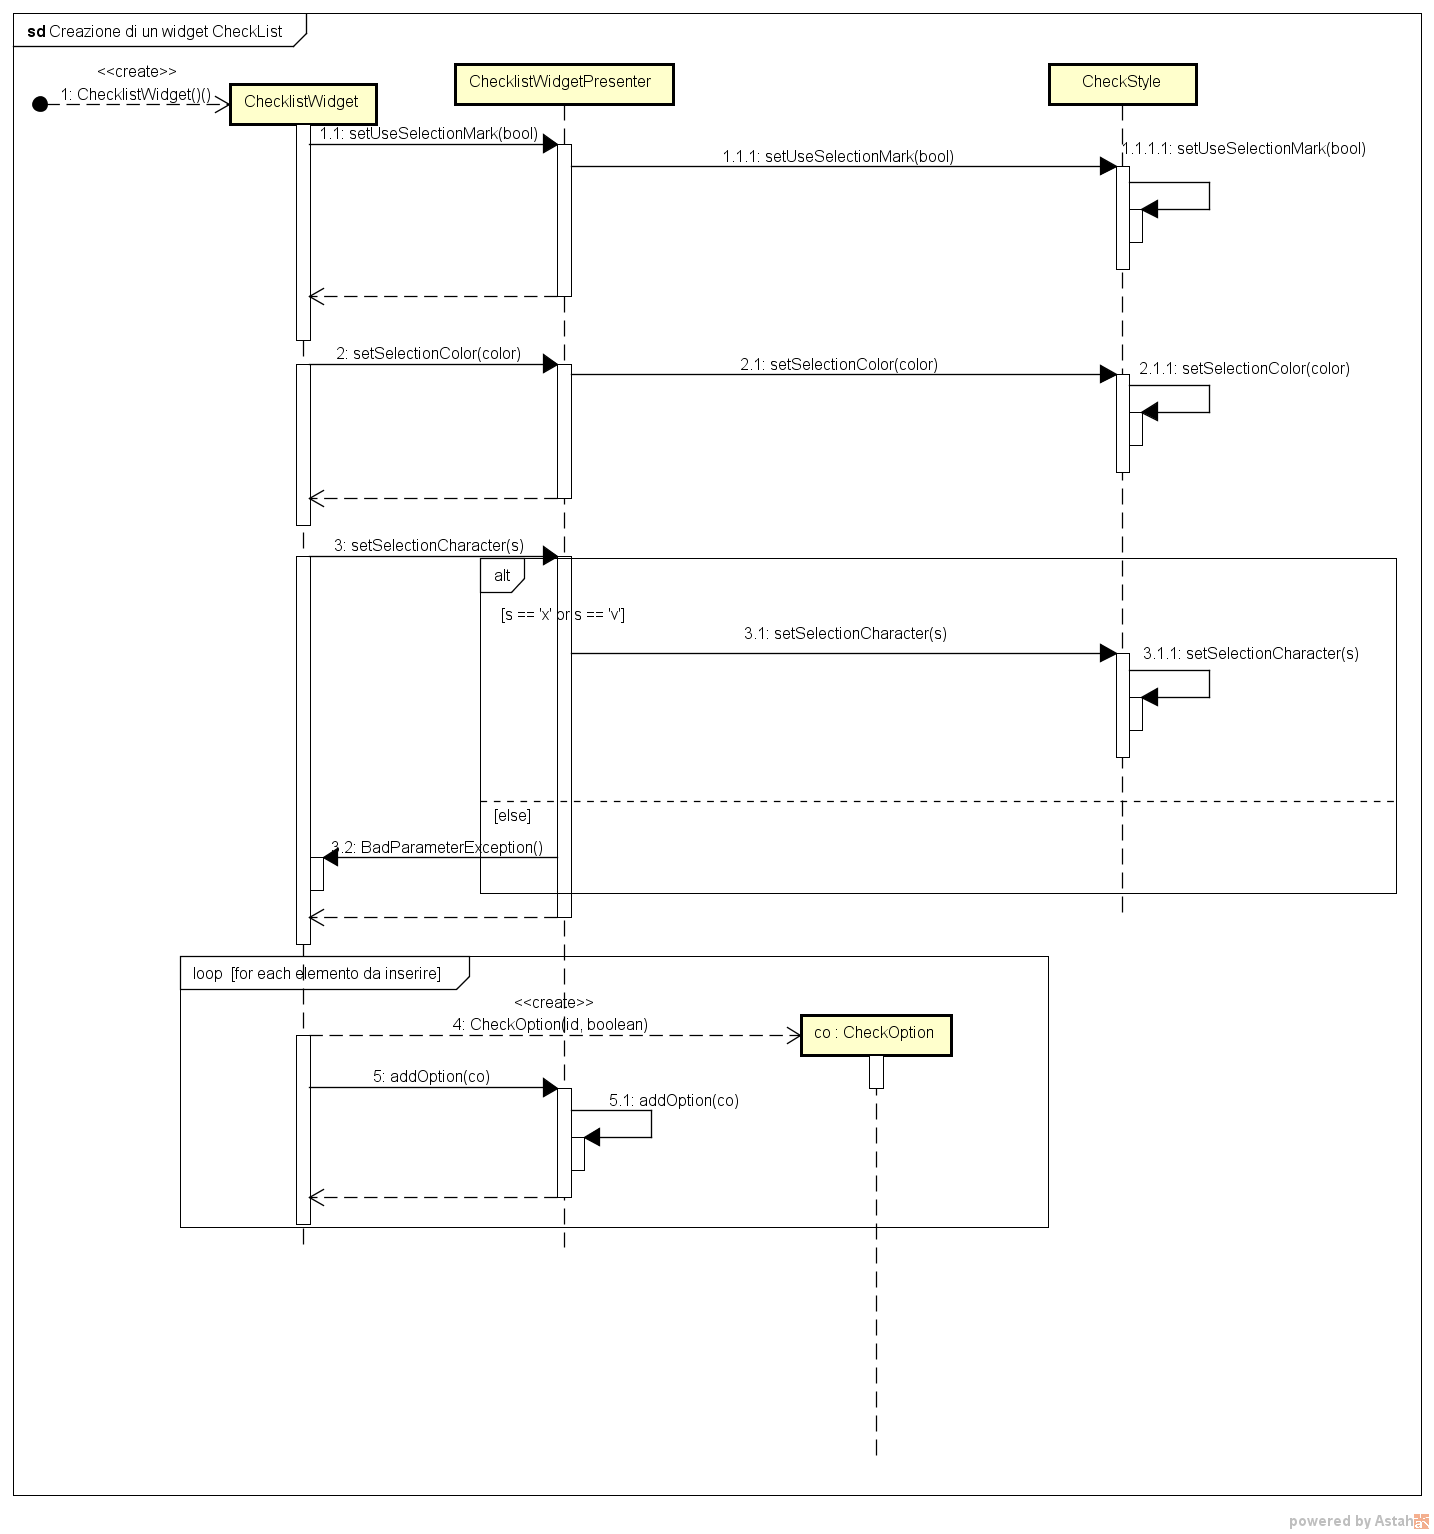
\includegraphics[width=16cm, height=14cm]{Sezioni/Diagrammi/img/Creazione di un widget CheckList.png}
	\caption{Creazione di un widget Checklist}
\end{figure}

Lo sviluppatore può creare un widget di tipo Checklist per aggiungerlo ad una sua ipotetica \termine{bolla}. Affinché non si verifichino errori, quando si usa il metodo \texttt{setSelectionCharacter} deve essere inserito correttamente un carattere per la spunta supportato. Inoltre se il flag \texttt{useSelectionMark} è stato impostato a false allora, indipendentemente dal carattere scelto dalla spunta, verrà usato il colore.\\
Le frecce di ritorno dal \texttt{ChecklistWidgetPresenter}  al \texttt{ChecklistWidget} sono state inserite poiché il cambiamento dei dati sul \termine{Presenter} ha effetto anche sulla View. La comunicazione tra queste due unità avviene tramite il \termine{framework} \termine{vue.js}. \\
Si noti, infine, che i metodi invocati da \texttt{Checklist} vengono chiamati in quest'ordine dal suo costruttore senza parametri. Tali metodi possono anche essere chiamati singolarmente dallo sviluppatore secondo l'ordine che egli preferisce. Queste azioni non verranno ulteriormente descritte poiché ritenute ridondanti.

\newpage

\subsubsection{Aggiungere un messaggio di completamento al widget Checklist}

\label{Aggiungere un messaggio di completamento al widget Checklist}
\begin{figure}[H]
	\centering
	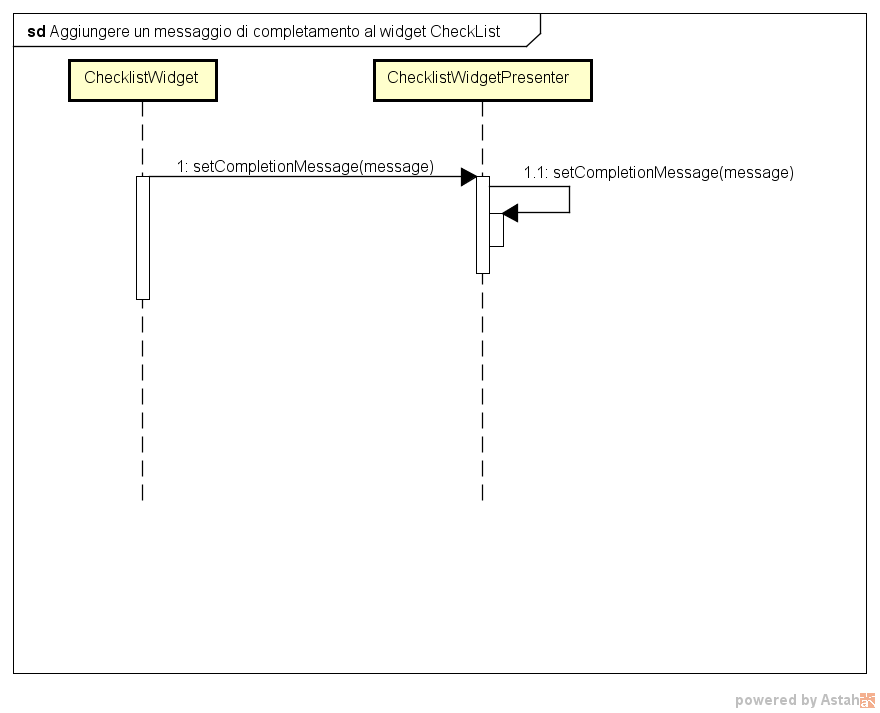
\includegraphics[width=16cm, height=14cm]{Sezioni/Diagrammi/img/Aggiungere un messaggio di completamento al widget Checklist.png}
	\caption{Aggiungere un messaggio di completamento al widget Checklist}
\end{figure}

Lo sviluppatore può aggiungere un messaggio di completamento per il widget Checklist. Questo messaggio verrà visualizzato non appena tutte le entry del widget saranno spuntate, ovvero al lancio dell'evento \texttt{emitOnCompletedList}.

\newpage

\subsubsection{Creazione di un widget bottone}

\label{Creazione di un widget bottone}
\begin{figure}[H]
	\centering
	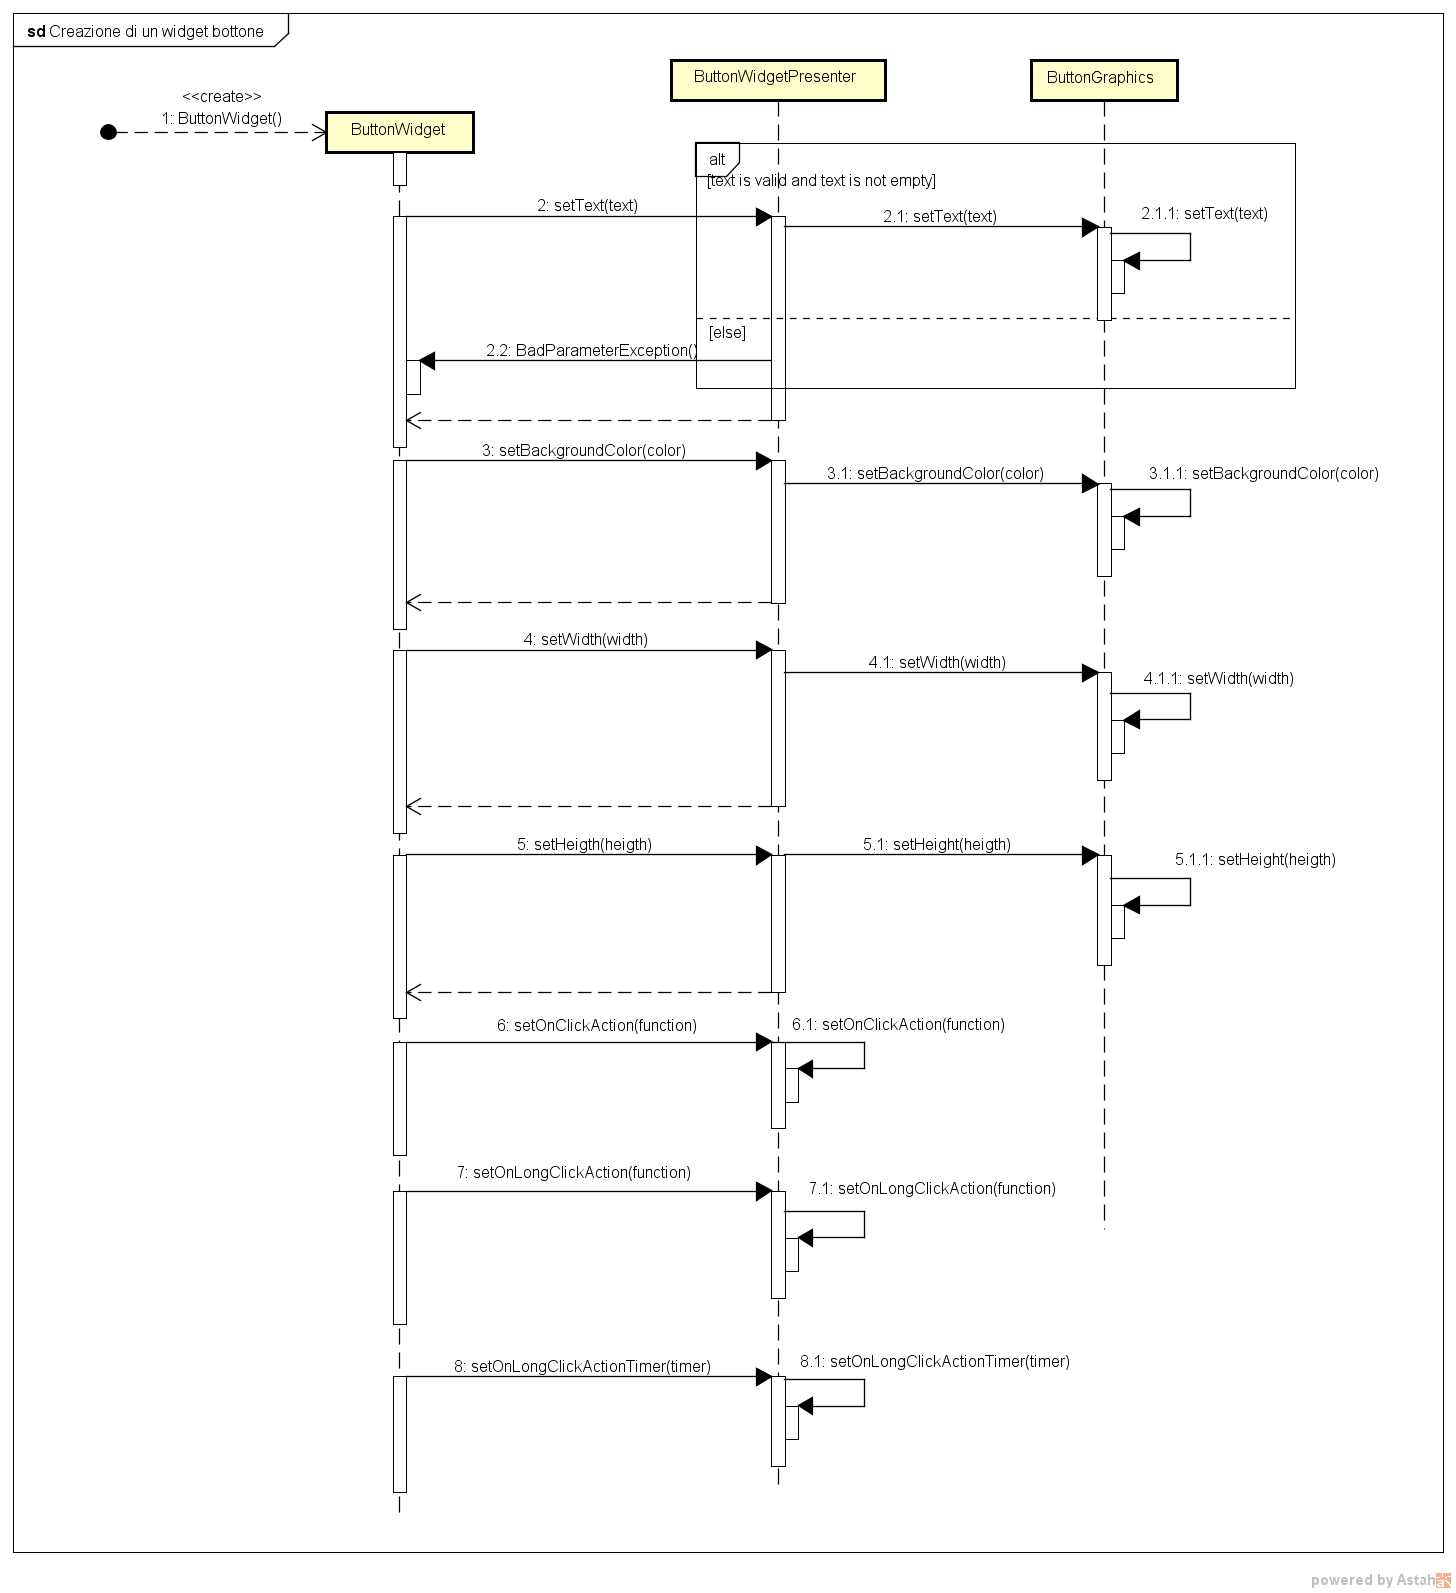
\includegraphics[width=16cm, height=14cm]{Sezioni/Diagrammi/img/Creazione di un widget bottone.png}
	\caption{Creazione di un widget bottone}
\end{figure}

Lo sviluppatore può creare un widget di tipo bottone per aggiungerlo ad una sua ipotetica \termine{bolla}. Se, durante la creazione del widget, il testo non dovesse essere impostato correttamente, il metodo \texttt{setText} di \texttt{ButtonWidgetPresenter} lancerà un'eccezione di tipo \texttt{BadParameterException}. \\
Le frecce di ritorno da \texttt{ButtonWidgetPresenter}  a \texttt{ButtonWidget} sono state inserite poiché il cambiamento dei dati sul \termine{Presenter} ha effetto anche sulla View. La comunicazione tra queste due unità avviene tramite il \termine{framework} \termine{vue.js}. \\
Si noti, infine, che i metodi invocati da \texttt{ButtonWidget} vengono chiamati in quest'ordine dal suo costruttore senza parametri. Tali metodi possono anche essere chiamati singolarmente dallo sviluppatore secondo l'ordine che egli preferisce. Queste azioni non verranno ulteriormente descritte poiché ritenute ridondanti.

\newpage

\subsubsection{Creazione di un listWidget}

\label{Click di un bottone}
\begin{figure}[H]
	\centering
	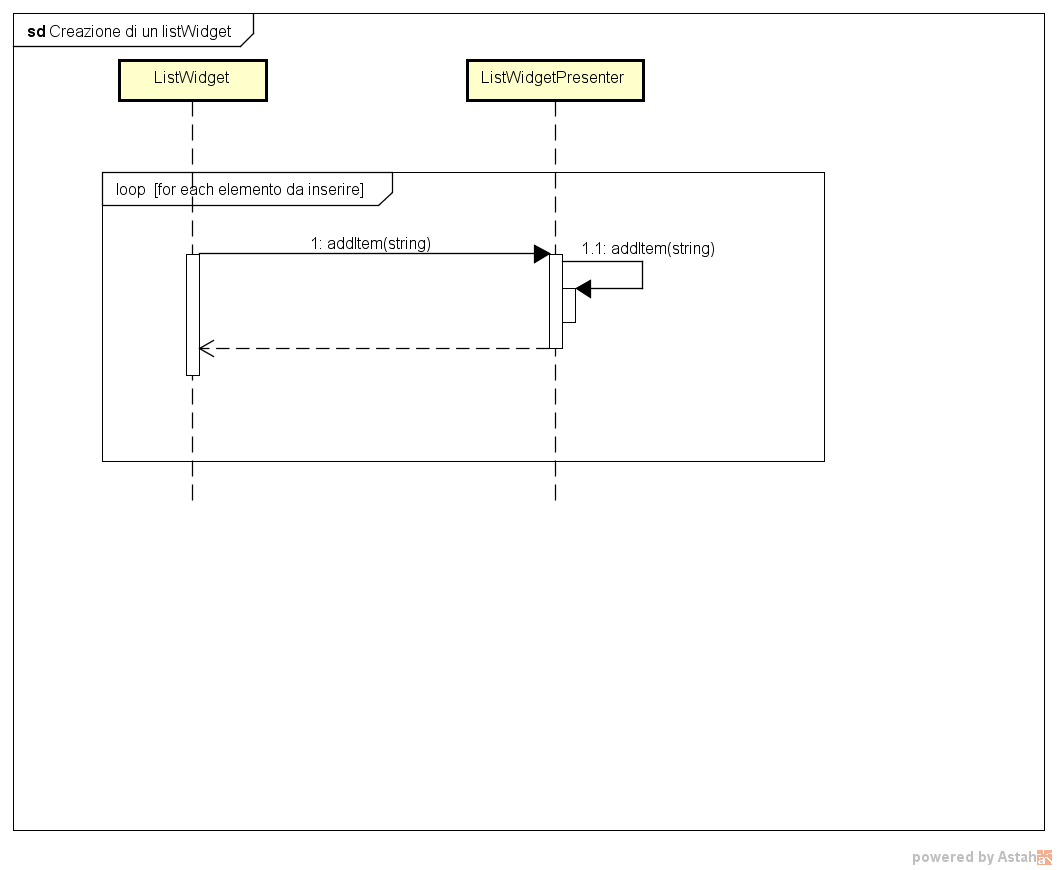
\includegraphics[width=16cm, height=14cm]{Sezioni/Diagrammi/img/Creazione di un listWidget.png}
	\caption{Creazione di un listWidget}
\end{figure}

Lo sviluppatore può creare un widget di tipo lista per aggiungerlo ad una sua ipotetica \termine{bolla}. Ogni elemento aggiunto logicamente dal presenter agisce anche sulla view. Per questo tipo di comunicazione si rimanda al \termine{framework} \termine{vue.js}. \\
L'azione compiuta per creare il widget può essere anche effettuata a posteriori della creazione del widget, questa però, essendo molto simile a quella appena descritta, viene omessa per ridondanza.

\newpage

\subsubsection{Creazione di una bolla aggiungendo un widget checklist}

\label{Creazione di una bolla aggiungendo un widget checklist}
\begin{figure}[H]
	\centering
	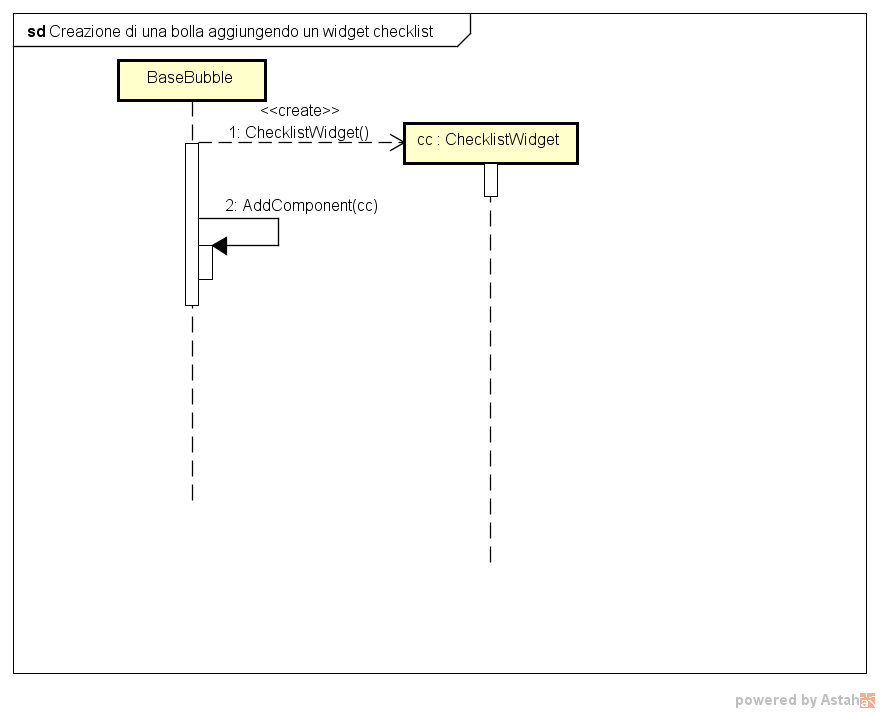
\includegraphics[width=16cm, height=14cm]{Sezioni/Diagrammi/img/Creazione di una bolla aggiungendo un widget checklist.png}
	\caption{Creazione di una bolla aggiungendo un widget checklist}
\end{figure}

Lo sviluppatore può aggiungere un widget alla \termine{bolla} appena creata. L'aggiunta dell'elemento avviene tramite il metodo \texttt{addComponent} che permette l'aggiunta sia di un layout che di un widget. Si noti che l'esempio è fatto con un widget specifico, ovvero il widget checklist, ma ciò vale per qualsiasi widget presente nell'\termine{SDK}. Gli altri esempi simili vengono, per questo motivo, omessi.

\newpage

\subsubsection{Aggiunta ad una bolla di un Layout contenente due widget di testo}

\label{Aggiunta ad una bolla di un Layout contenente due widget di testo}
\begin{figure}[H]
	\centering
	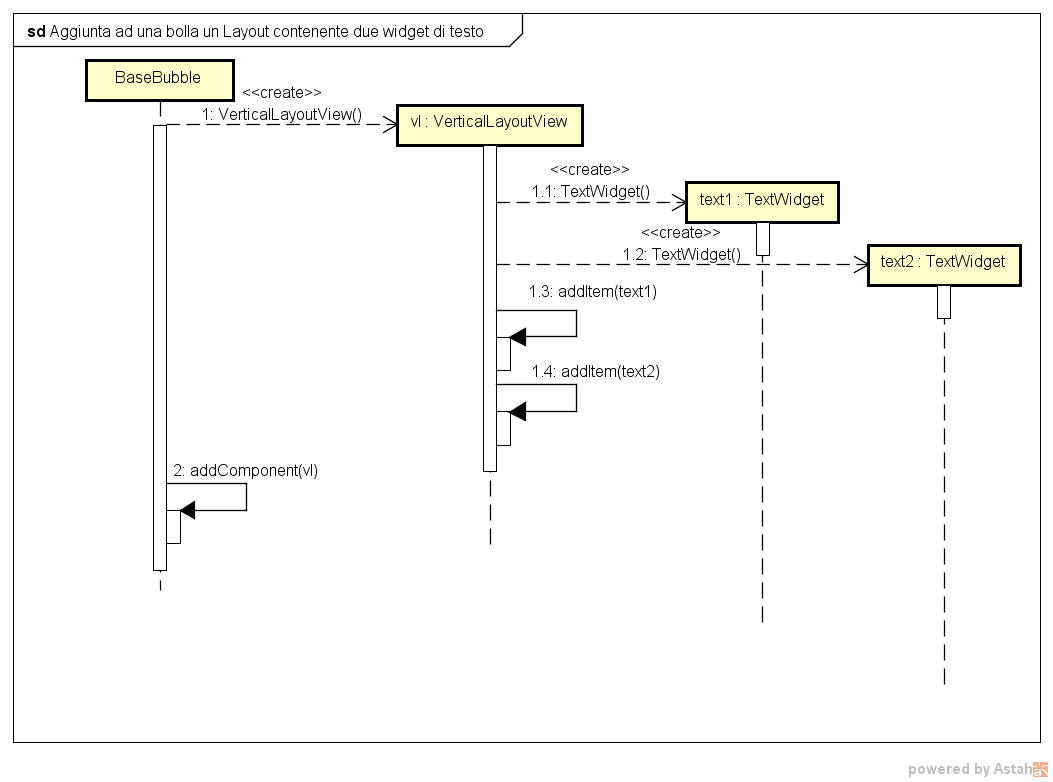
\includegraphics[width=16cm, height=14cm]{Sezioni/Diagrammi/img/Aggiunta ad una bolla un Layout contenente due widget di testo.png}
	\caption{Aggiunta ad una bolla di un Layout contenente due widget di testo}
	
\end{figure}
Lo sviluppatore può aggiungere un layout contenente dei widgets alla \termine{bolla}. Anche questo rappresenta solo un generico esempio di come si possa aggiungere un layout ad una \termine{bolla}. Gli altri esempi simili saranno dunque omessi. 

\newpage

\subsubsection{Creazione di una bolla MarkDownBubble}

\label{Creazione di una bolla MarkDownBubble}
\begin{figure}[H]
	\centering
	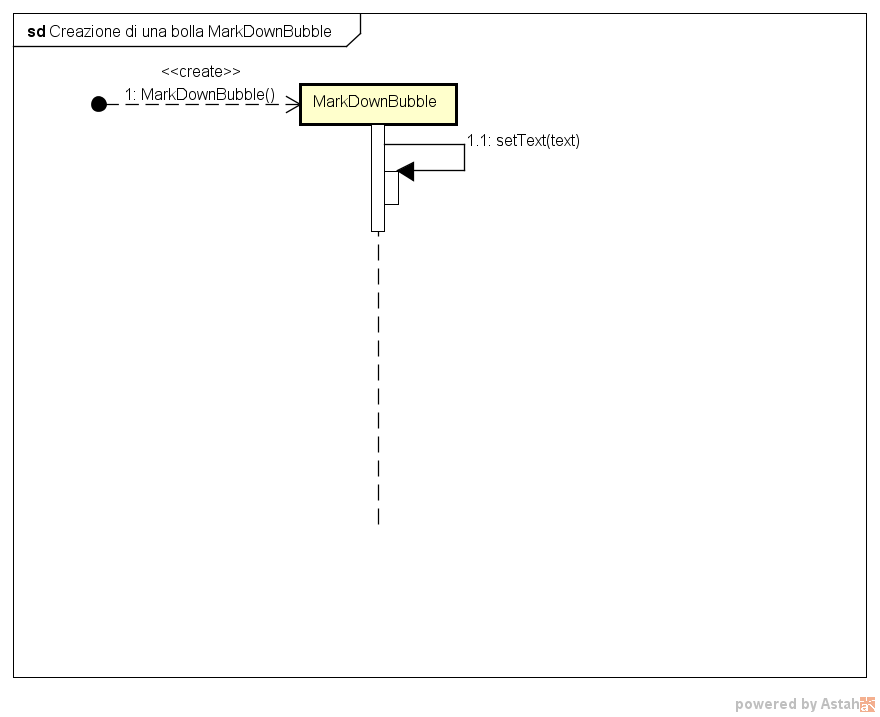
\includegraphics[width=12cm, height=8cm]{Sezioni/Diagrammi/img/Creazione di una bolla MarkDownBubble.png}
	\caption{Creazione di una bolla MarkDownBubble}
	
\end{figure}

Lo sviluppatore può creare una \termine{bolla} MarkDownBubble disponibile nell'\termine{SDK}.

\subsubsection{Creazione di una bolla AlertBubble}

\label{Creazione di una bolla AlertBubble}
\begin{figure}[H]
	\centering
	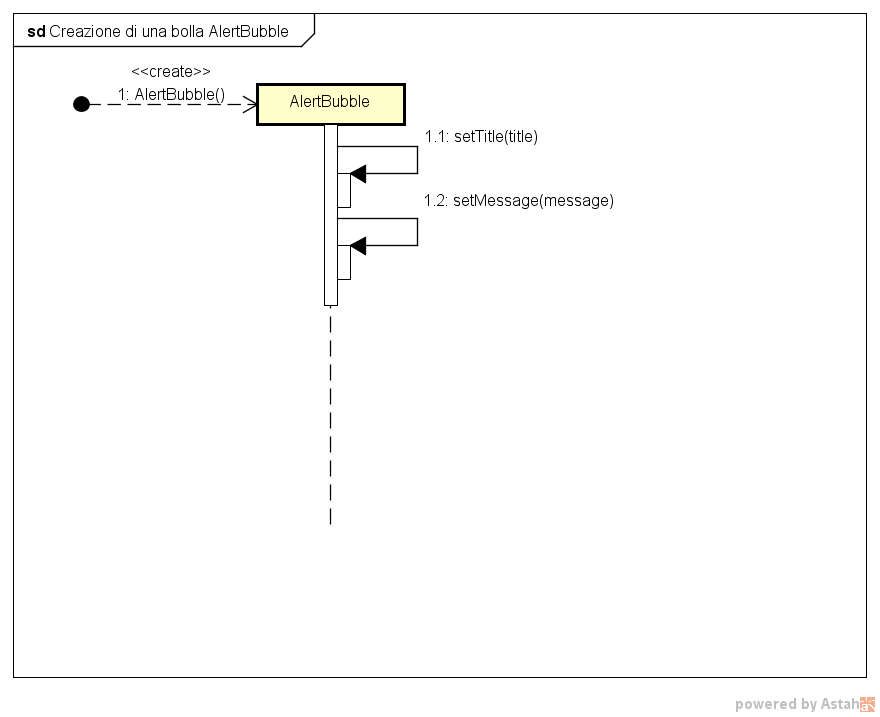
\includegraphics[width=12cm, height=8cm]{Sezioni/Diagrammi/img/Creazione di una bolla AlertBubble.png}
	\caption{Creazione di una bolla AlertBubble}
	
\end{figure}

Lo sviluppatore può creare una \termine{bolla} AlertBubble disponibile nell'\termine{SDK}.

\newpage

\subsubsection{Creazione di una bolla ToDoListBubble}

\label{Creazione di una bolla ToDoListBubble}
\begin{figure}[H]
	\centering
	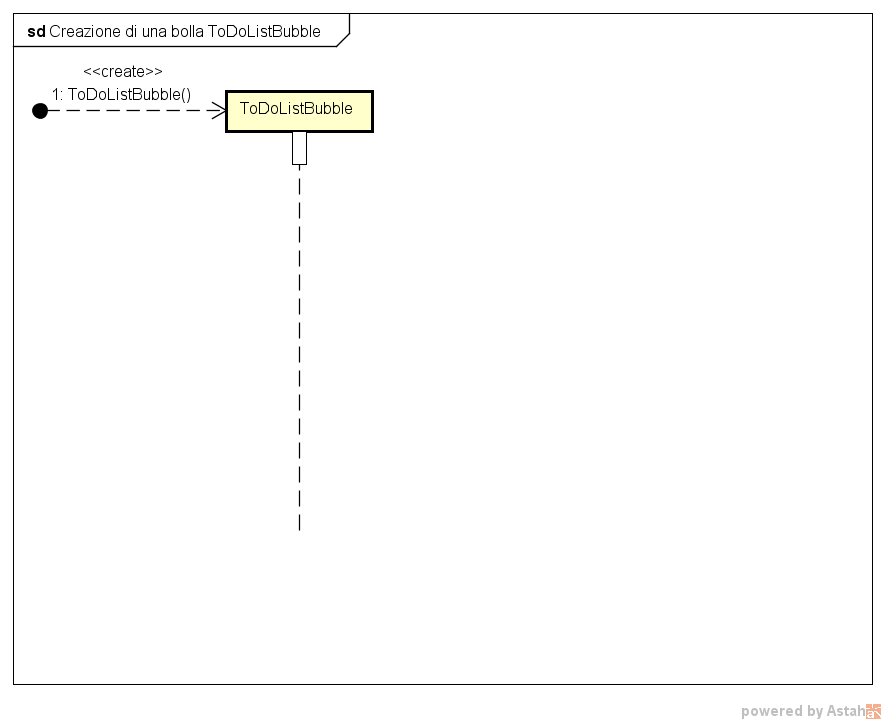
\includegraphics[width=12cm, height=8cm]{Sezioni/Diagrammi/img/Creazione di una bolla ToDoListBubble.png}
	\caption{Creazione di una bolla ToDoListBubble}
	
\end{figure}

Lo sviluppatore può creare una \termine{bolla} ToDoListBubble disponibile nell'\termine{SDK}.



\subsection{Package application}
\label{Package application}
\begin{figure}[H]
	\centering
	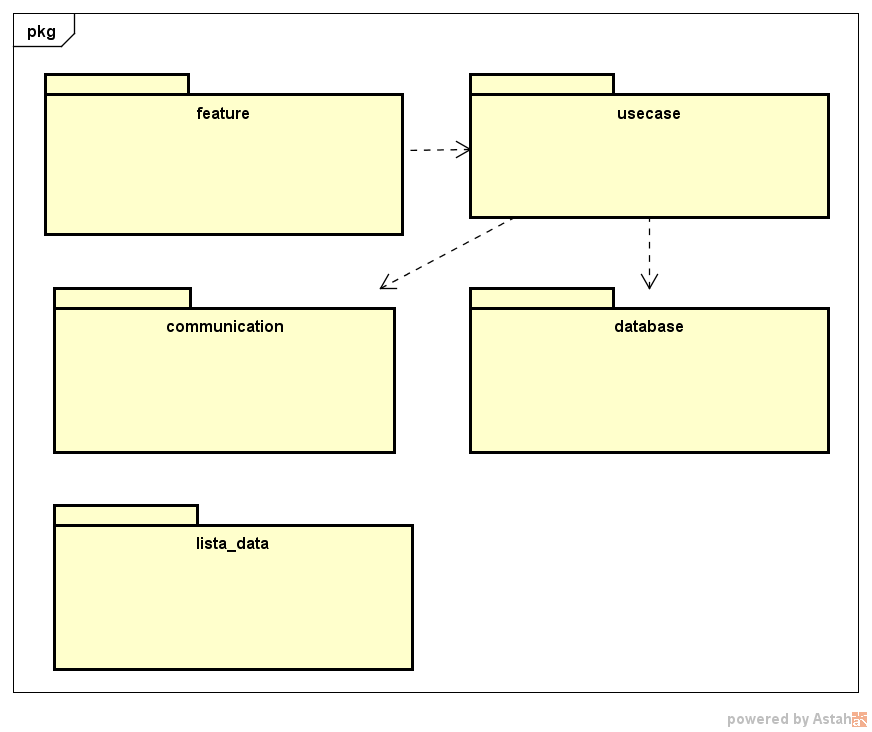
\includegraphics[scale=0.5]{Sezioni/Packages/App/application.png}
	\caption{Package application}
\end{figure}
\begin{itemize}
	\item \textbf{Descrizione}: \termine{Package} contenente tutti i file dell'applicazione demo.
	\item \textbf{Classi e packages contenuti}:
	\begin{itemize}
		\item application::feature: package contenente tutte le feature principali dell'applicazione
		\item application::usecase: package contenente tutti gli usecase dell'applicazione
		\item application::lista\_data: package contenente le classi che modellano i dati dell'applicazione
		\item application::database: package contenente tutte le classi relative ai database
	\end{itemize}
	\item application::communication: package contenente tutte le classi atte a comunicare con la chat
\end{itemize}


\subsubsection{Package application::usecase}
\label{Package application::usecase}
\begin{figure}[H]
	\centering
	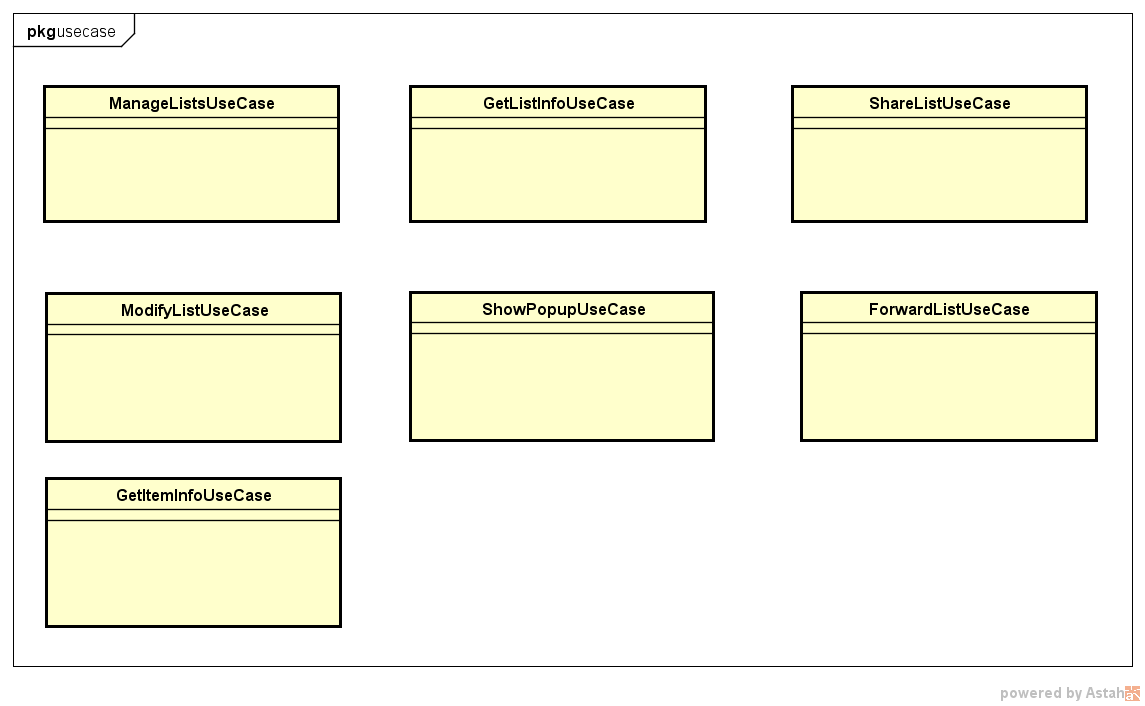
\includegraphics[scale=0.5]{Sezioni/Packages/App/usecase.png}
	\caption{Package application::usecase}
\end{figure}
\begin{itemize}
	\item \textbf{Descrizione}: package contenente tutte le classi che gestiscono la logica dell'applicazione
	\item \textbf{Classi e packages contenuti}:
	\begin{itemize}
	\item application::usecase::ManageListsUseCase: classe che gestisce le modifiche alle liste memorizzate nel database
	\item application::usecase GetListInfoUseCase: classe che recupera i dati di una lista dal database
	\item application::usecase:ModifyListUseCase: classe che permette la modifica di una lista memorizzata all'interno del database
	\item application::usecase ShowPopupUseCase: classe che permette la visualizzazione di finestre modali
	\item application::usecase::GetItemInfoUseCase: classe che permette di recuperare le informazioni di un particolare oggetto in una lista dal database
	\end{itemize}
\end{itemize}

\subsubsection{Package application::lista\_data}
\label{Package application::lista_data}
\begin{figure}[H]
	\centering
	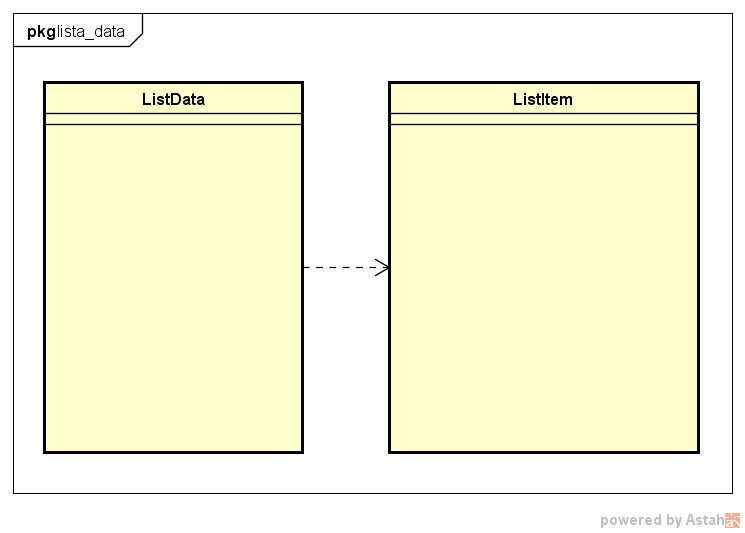
\includegraphics[scale=0.5]{Sezioni/Packages/App/lista_data.png}
	\caption{Package application::lista\_data}
\end{figure}
\begin{itemize}
	\item \textbf{Descrizione}: package contenente tutte le classi che modellano gli oggetti di una lista e di un oggetti di una lista
	\item \textbf{Classi e packages contenuti}:
	\begin{itemize}
	\item application::lista\_data::ListData: classe che modella una lista
	\item application::lista\_data::ListItem: classe che modella un oggetto di una lista
	\end{itemize}
\end{itemize}

\subsubsection{Package application::communication}
\label{Package application::communication}
\begin{figure}[H]
	\centering
	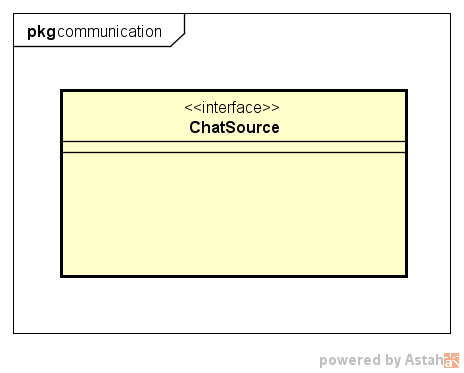
\includegraphics[scale=0.5]{Sezioni/Packages/App/communication.png}
	\caption{Package application::communication}
\end{figure}
\begin{itemize}
	\item \textbf{Descrizione}: package che contiene le classi di comunicazione con l'istanza di Rocket.chat
	\item \textbf{Classi e packages contenuti}:
	\begin{itemize}
	\item application::communication::ChatSource: interfaccia che permette la comunicazione con l'istanza di Rocket.chat
	\end{itemize}
\end{itemize}

\subsubsection{Package application::database}
\label{Package application::database}
\begin{figure}[H]
	\centering
	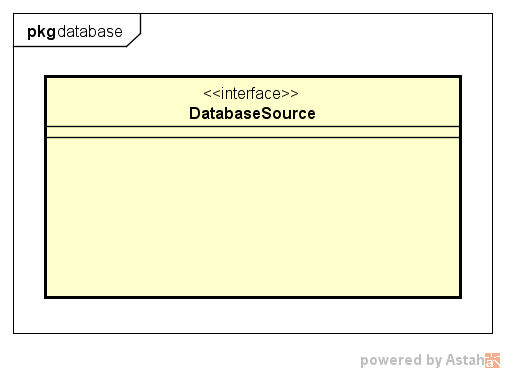
\includegraphics[scale=0.5]{Sezioni/Packages/App/database.png}
	\caption{Package application::database}
\end{figure}
\begin{itemize}
	\item \textbf{Descrizione}: package che contiene le classi per interfacciarsi con il database all'interno del quale sono salvati i dati delle liste
	\item \textbf{Classi e packages contenuti}:
	\begin{itemize}
	\item application::database::DatabaseSource: interfaccia che permette la comunicazione con il database all'interno del quale sono salvati i dati delle varie liste
	\end{itemize}
\end{itemize}

\subsubsection{Package application::feature::add\_item}
\label{Package application::feature::add_item}
\begin{figure}[H]
	\centering
	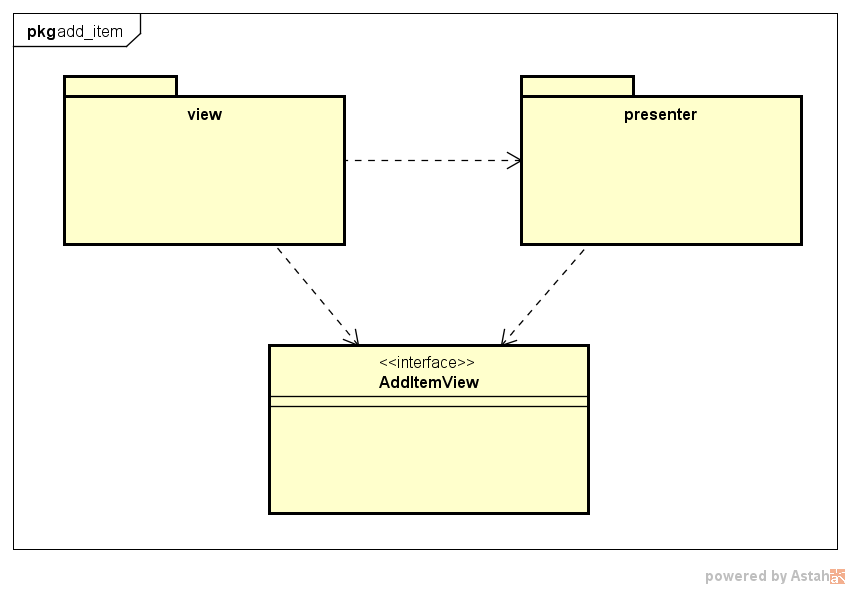
\includegraphics[scale=0.5]{Sezioni/Packages/App/add_item.png}
	\caption{Package application::feature::add\_item}
\end{figure}
\begin{itemize}
	\item \textbf{Descrizione}: package contenente i file relativi alla funzionalità di aggiunta elemento ad una lista
	\item \textbf{Classi e packages contenuti}:
	\begin{itemize}
	\item application::feature::add\_item::view: package contenente la view per l'aggiunta di un elemento
	\item application::feature::add\_item::presenter: package contenente il presenter per la view di aggiunta elemento
	\item application::feature::add\_item::AddItemView: interfaccia che rappresenta la vista di aggiunta oggetto
	\end{itemize}
\end{itemize}

\subsubsection{Package application::feature::add\_item::view}
\label{Package application::feature::add_item::view}
\begin{figure}[H]
	\centering
	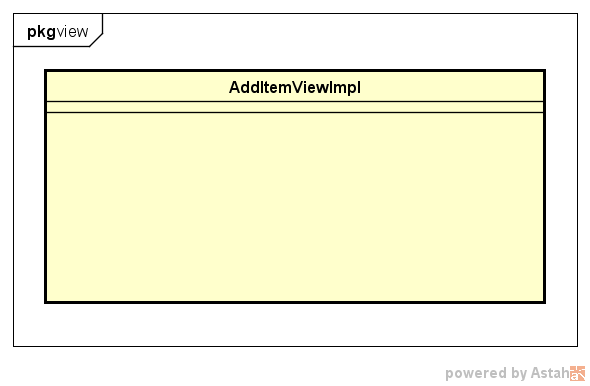
\includegraphics[scale=0.5]{Sezioni/Packages/App/add_item_view.png}
	\caption{Package application::feature::add\_item::view}
\end{figure}
\begin{itemize}
	\item \textbf{Descrizione}: package contenente la view per l'aggiunta di un elemento
	\item \textbf{Classi e packages contenuti}:
	\begin{itemize}
	\item application::feature::add\_item::view::AddItemViewImpl: implementazione dell'interfaccia AddItemView che rappresenta la vista di aggiunta di un oggetto alla lista
	\end{itemize}
\end{itemize}

\subsubsection{Package application::feature::add\_item::presenter}
\label{Package application::feature::add_item::presenter}
\begin{figure}[H]
	\centering
	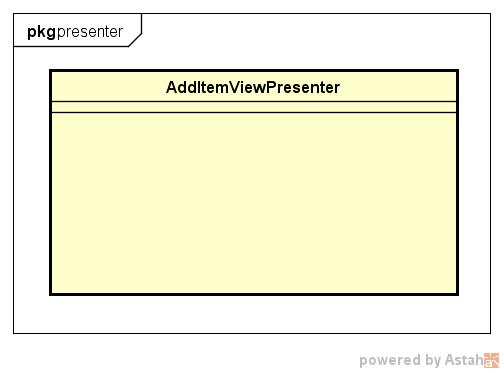
\includegraphics[scale=0.5]{Sezioni/Packages/App/add_item_presenter.png}
	\caption{Package application::feature::add\_item::presenter}
\end{figure}
\begin{itemize}
	\item \textbf{Descrizione}: package contenente il presenter per la vista di aggiunta di un oggetto alla lista
	\item \textbf{Classi e packages contenuti}:
	\begin{itemize}
	\item application::feature::add\_item::presenter::AddItemViewPresenter: presenter per la vista di aggiunta di un oggetto alla lista
	\end{itemize}
\end{itemize}

\subsubsection{Package application::feature::change\_list\_info}
\label{Package application::feature::change_list_info}
\begin{figure}[H]
	\centering
	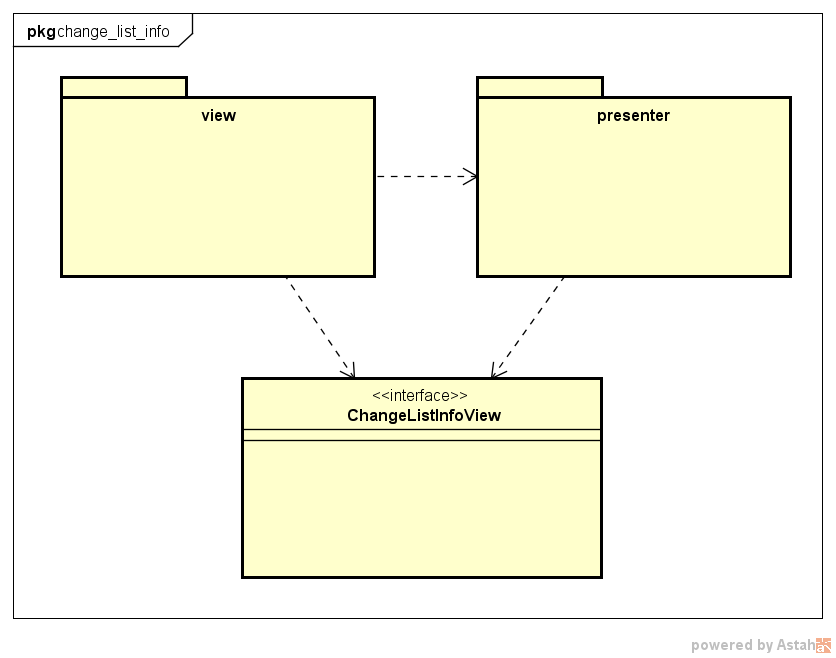
\includegraphics[scale=0.5]{Sezioni/Packages/App/change_list_info.png}
	\caption{Package application::feature::change\_list\_info}
\end{figure}
\begin{itemize}
	\item \textbf{Descrizione}: package contenente i componenti per la funzionalità di modifica informazioni di una lista
	\item \textbf{Classi e packages contenuti}:
	\begin{itemize}
	\item application::feature::change\_list\_info::view: package contenente la vista per la modifica informazioni di una lista
	\item application::feature::change\_list\_info::presenter: package contenente il presenter per la vista di modifica informazioni di una lista
	\item application::feature::change\_list\_info::ChangeListInfoView: interfaccia rappresentante la vista per la modifica informazioni di una lista
	\end{itemize}
\end{itemize}

\subsubsection{Package application::feature::change\_list\_info::view}
\label{Package application::feature::change_list_info::view}
\begin{figure}[H]
	\centering
	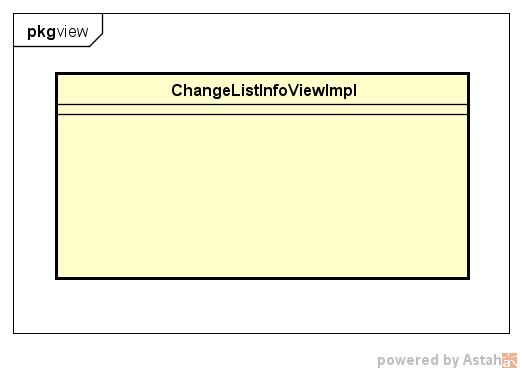
\includegraphics[scale=0.5]{Sezioni/Packages/App/change_list_info_view.png}
	\caption{Package application::feature::change\_list\_info::view}
\end{figure}
\begin{itemize}
	\item \textbf{Descrizione}: package contenente la vista per la funzionalità di modifica informazioni di una lista
	\item \textbf{Classi e packages contenuti}:
	\begin{itemize}
	\item application::feature::change\_list\_info::view::ChangeListInfoViewImpl: implementazione dell'interfaccia che rappresenta la vista per la funzionalità di modifica della informazioni di una lista
	\end{itemize}
\end{itemize}

\subsubsection{Package application::feature::change\_list\_info::presenter}
\label{Package application::feature::change_list_info::presenter}
\begin{figure}[H]
	\centering
	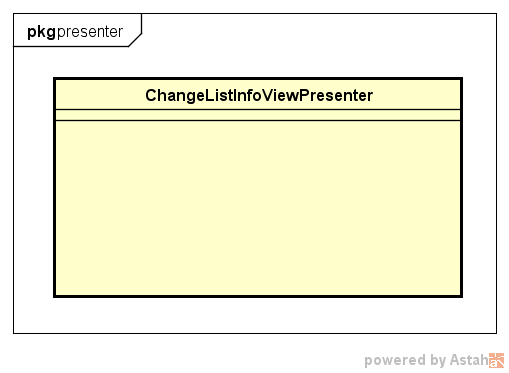
\includegraphics[scale=0.5]{Sezioni/Packages/App/change_list_info_presenter.png}
	\caption{Package application::feature::change\_list\_info::presenter}
\end{figure}
\begin{itemize}
	\item \textbf{Descrizione}: package contenente il presenter per la vista di modifica informazioni di una lista
	\item \textbf{Classi e packages contenuti}:
	\begin{itemize}
	\item application::feature::change\_list\_info::presenter::ChangeListInfoViewPresenter: classe che rappresenta il presenter per la vista di modifica dei dati di una lista
	\end{itemize}
\end{itemize}


\subsubsection{Package application::feature::create\_list}
\label{Package application::feature::create_list}
\begin{figure}[H]
	\centering
	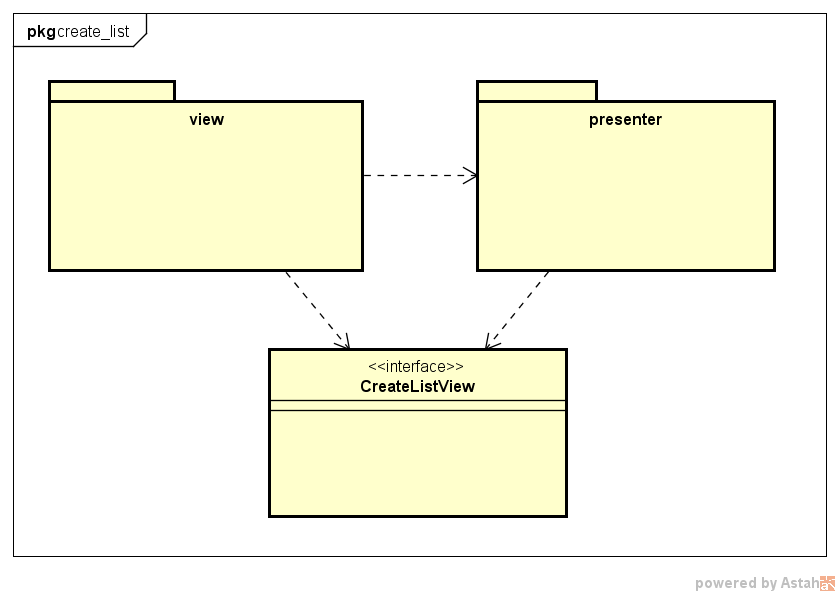
\includegraphics[scale=0.5]{Sezioni/Packages/App/create_list.png}
	\caption{Package application::feature::create\_list}
\end{figure}
\begin{itemize}
	\item \textbf{Descrizione}: package contenente i componenti per la funzionalità di creazione di una lista
	\item \textbf{Classi e packages contenuti}:
	\begin{itemize}
	\item application::feature::create\_list::view: package contenente la vista per la creazione di una lista
	\item application::feature::create\_list::presenter: package contenente il presenter per la vista di creazione di una lista
	\item application::feature::create\_list::CreateListView: interfaccia rappresentante la vista per la creazione di una lista
	\end{itemize}
\end{itemize}

\subsubsection{Package application::feature::create\_list::view}
\label{Package application::feature::create_list::view}
\begin{figure}[H]
	\centering
	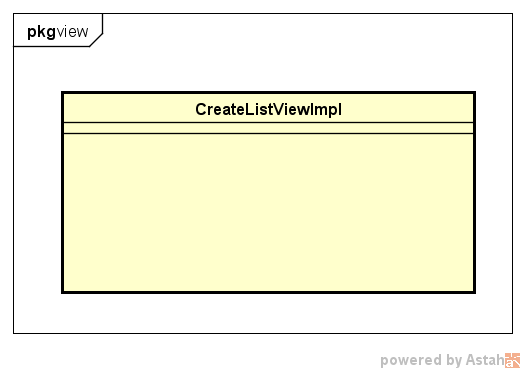
\includegraphics[scale=0.5]{Sezioni/Packages/App/create_list_view.png}
	\caption{Package application::feature::create\_list::view}
\end{figure}
\begin{itemize}
	\item \textbf{Descrizione}: package contenente la vista per la funzionalità di creazione di una lista
	\item \textbf{Classi e packages contenuti}:
	\begin{itemize}
	\item application::feature::create\_list::view::CreateListViewImpl: implementazione dell'interfaccia che rappresenta la vista per la funzionalità di creazione di una lista
	\end{itemize}
\end{itemize}

\subsubsection{Package application::feature::create\_list::presenter}
\label{Package application::feature::create_list::presenter}
\begin{figure}[H]
	\centering
	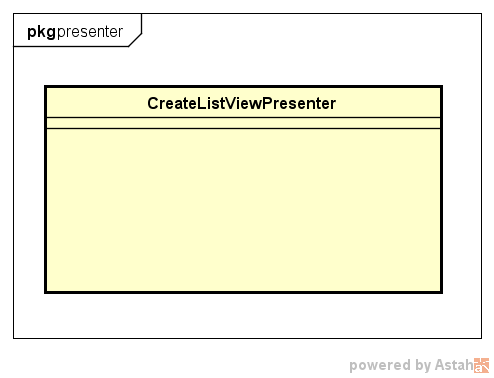
\includegraphics[scale=0.5]{Sezioni/Packages/App/create_list_presenter.png}
	\caption{Package application::feature::create\_list::presenter}
\end{figure}
\begin{itemize}
	\item \textbf{Descrizione}: package contenente il presenter per la vista di creazione di una lista
	\item \textbf{Classi e packages contenuti}:
	\begin{itemize}
	\item application::feature::create\_list::presenter::CreateListViewPresenter: classe che rappresenta il presenter per la vista di creazione di una lista
	\end{itemize}
\end{itemize}

\subsubsection{Package application::feature::forward}
\label{Package application::feature::forward}
\begin{figure}[H]
	\centering
	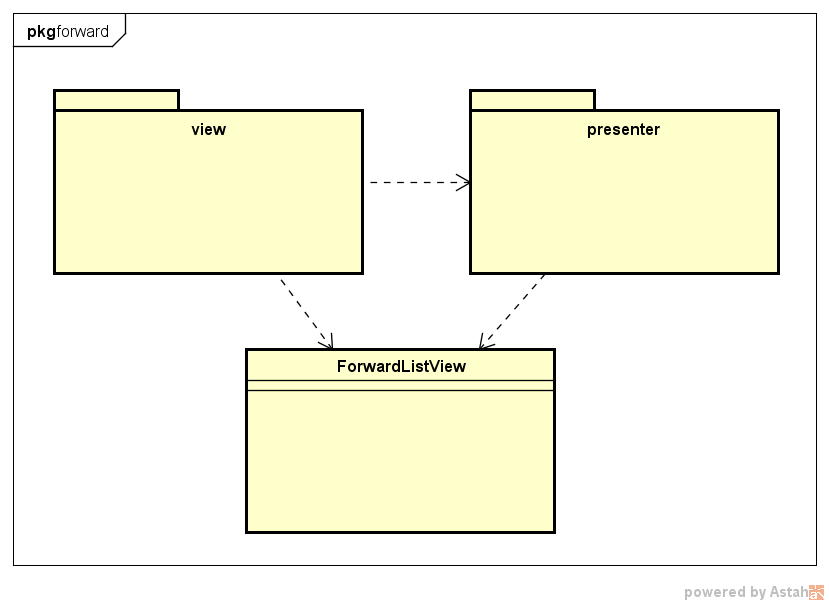
\includegraphics[scale=0.5]{Sezioni/Packages/App/forward.png}
	\caption{Package application::feature::forward}
\end{figure}
\begin{itemize}
	\item \textbf{Descrizione}: package contenente i componenti per la funzionalità di inoltro di una lista
	\item \textbf{Classi e packages contenuti}:
	\begin{itemize}
	\item application::feature::forward::view: package contenente la vista per la inoltro di una lista
	\item application::feature::forward::presenter: package contenente il presenter per la vista di inoltro di una lista
	\item application::feature::forward::ForwardListView: interfaccia rappresentante la vista per la funzionalità inoltro di una lista
	\end{itemize}
\end{itemize}

\subsubsection{Package application::feature::forward::view}
\label{Package application::feature::forward::view}
\begin{figure}[H]
	\centering
	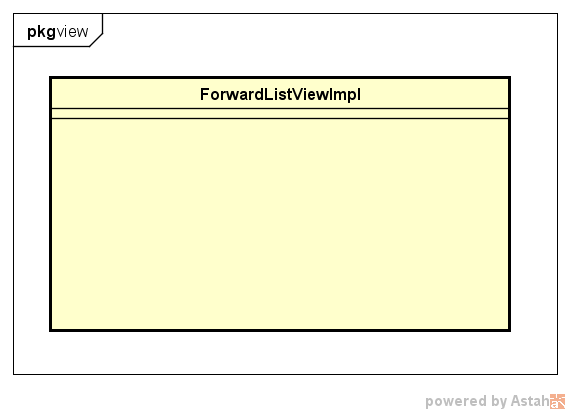
\includegraphics[scale=0.5]{Sezioni/Packages/App/forward_view.png}
	\caption{Package application::feature::forward::view}
\end{figure}
\begin{itemize}
	\item \textbf{Descrizione}: package contenente la vista per la funzionalità di inoltro di una lista
	\item \textbf{Classi e packages contenuti}:
	\begin{itemize}
	\item application::feature::forward::view::ForwardListViewImpl: implementazione dell'interfaccia che rappresenta la vista per la funzionalità di inoltro di una lista
	\end{itemize}
\end{itemize}

\subsubsection{Package application::feature::forward::presenter}
\label{Package application::feature::forward::presenter}
\begin{figure}[H]
	\centering
	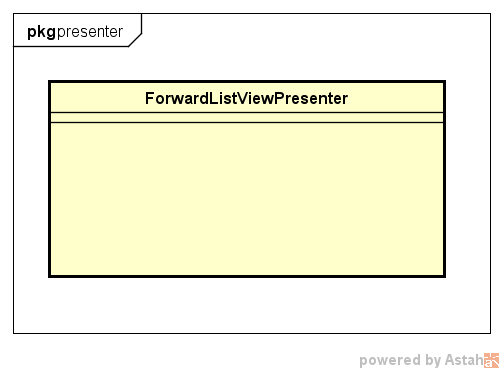
\includegraphics[scale=0.5]{Sezioni/Packages/App/forward_presenter.png}
	\caption{Package application::feature::forward::presenter}
\end{figure}
\begin{itemize}
	\item \textbf{Descrizione}: package contenente il presenter per la vista di inoltro di una lista
	\item \textbf{Classi e packages contenuti}:
	\begin{itemize}
	\item application::feature::forward::presenter::ForwardListViewPresenter: classe che rappresenta il presenter per la vista di inoltro di una lista
	\end{itemize}
\end{itemize}

\subsubsection{Package application::feature::input\_item\_info}
\label{Package application::feature::input_item_info}
\begin{figure}[H]
	\centering
	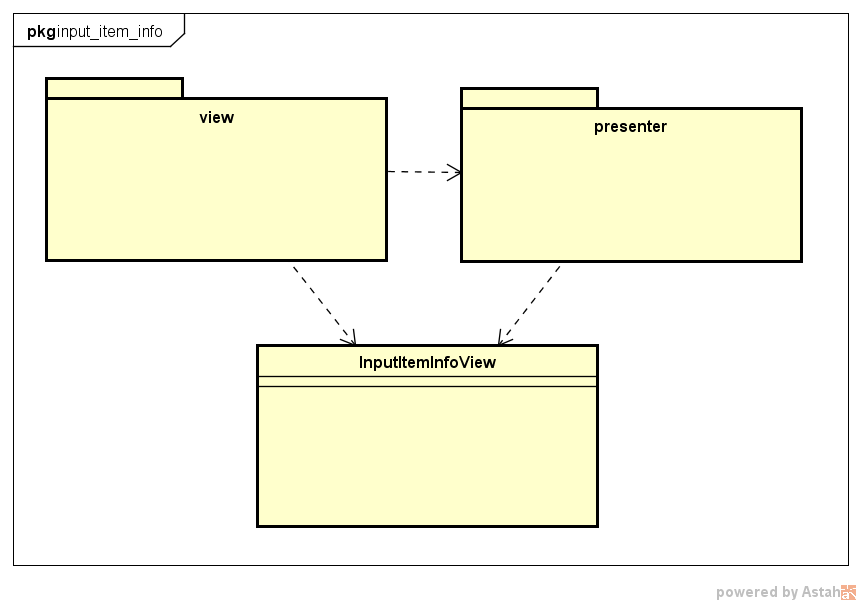
\includegraphics[scale=0.5]{Sezioni/Packages/App/input_item_info.png}
	\caption{Package application::feature::input\_item\_info}
\end{figure}
\begin{itemize}
	\item \textbf{Descrizione}: package contenente i componenti per la funzionalità di inserimento dati di un oggetto della lista
	\item \textbf{Classi e packages contenuti}:
	\begin{itemize}
	\item application::feature::input\_item\_info::view: package contenente la vista per la inserimento dati di un oggetto della lista
	\item application::feature::input\_item\_info::presenter: package contenente il presenter per la vista di inserimento dati di un oggetto della lista
	\item application::feature::input\_item\_info::InputItemInfoView: interfaccia rappresentante la vista per la funzionalità inserimento dati di un oggetto della lista
	\end{itemize}
\end{itemize}

\subsubsection{Package application::feature::input\_item\_info::view}
\label{Package application::feature::input_item_info::view}
\begin{figure}[H]
	\centering
	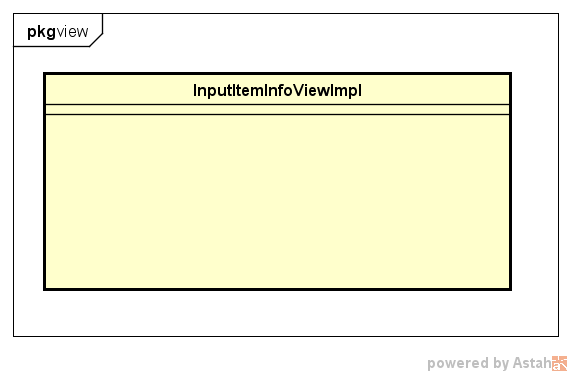
\includegraphics[scale=0.5]{Sezioni/Packages/App/input_item_info_view.png}
	\caption{Package application::feature::input\_item\_info::view}
\end{figure}
\begin{itemize}
	\item \textbf{Descrizione}: package contenente la vista per la funzionalità di inserimento dati di un oggetto della lista
	\item \textbf{Classi e packages contenuti}:
	\begin{itemize}
	\item application::feature::input\_item\_info::view::InputItemInfoViewImpl: implementazione dell'interfaccia che rappresenta la vista per la funzionalità di inserimento dati di un oggetto della lista
	\end{itemize}
\end{itemize}

\subsubsection{Package application::feature::input\_item\_info::presenter}
\label{Package application::feature::input_item_info::presenter}
\begin{figure}[H]
	\centering
	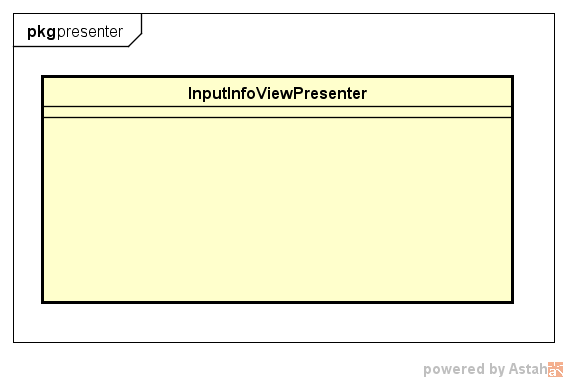
\includegraphics[scale=0.5]{Sezioni/Packages/App/input_item_info_presenter.png}
	\caption{Package application::feature::input\_item\_info::presenter}
\end{figure}
\begin{itemize}
	\item \textbf{Descrizione}: package contenente il presenter per la vista di inserimento dati di un oggetto della lista
	\item \textbf{Classi e packages contenuti}:
	\begin{itemize}
	\item application::feature::input\_item\_info::presenter::InputItemInfoViewPresenter: classe che rappresenta il presenter per la vista di inserimento dati di un oggetto della lista
	\end{itemize}
\end{itemize}


\subsubsection{Package application::feature::input\_list\_info}
\label{Package application::feature::input_list_info}
\begin{figure}[H]
	\centering
	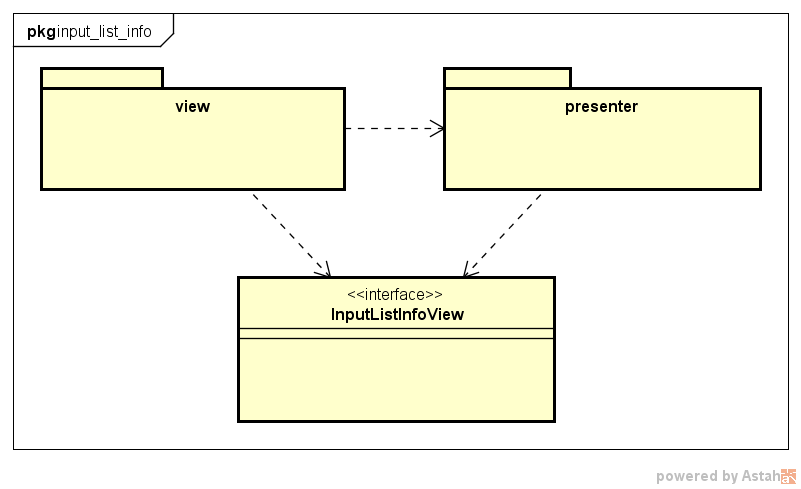
\includegraphics[scale=0.5]{Sezioni/Packages/App/input_list_info.png}
	\caption{Package application::feature::input\_list\_info}
\end{figure}
\begin{itemize}
	\item \textbf{Descrizione}: package contenente i componenti per la funzionalità di inserimento dati di una lista
	\item \textbf{Classi e packages contenuti}:
	\begin{itemize}
	\item application::feature::input\_list\_info::view: package contenente la vista per la inserimento dati di una lista
	\item application::feature::input\_list\_info::presenter: package contenente il presenter per la vista di inserimento dati di una lista
	\item application::feature::input\_list\_info::InputListInfoView: interfaccia rappresentante la vista per la funzionalità inserimento dati di una lista
	\end{itemize}
\end{itemize}

\subsubsection{Package application::feature::input\_list\_info::view}
\label{Package application::feature::input_list_info::view}
\begin{figure}[H]
	\centering
	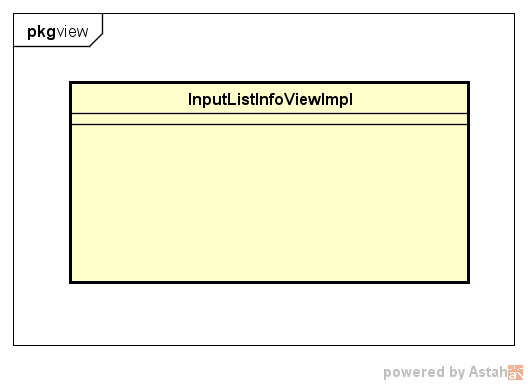
\includegraphics[scale=0.5]{Sezioni/Packages/App/input_list_info_view.png}
	\caption{Package application::feature::input\_list\_info::view}
\end{figure}
\begin{itemize}
	\item \textbf{Descrizione}: package contenente la vista per la funzionalità di inserimento dati di una lista
	\item \textbf{Classi e packages contenuti}:
	\begin{itemize}
	\item application::feature::input\_list\_info::view::InputListInfoViewImpl: implementazione dell'interfaccia che rappresenta la vista per la funzionalità di inserimento dati di una lista
	\end{itemize}
\end{itemize}

\subsubsection{Package application::feature::input\_list\_info::presenter}
\label{Package application::feature::input_list_info::presenter}
\begin{figure}[H]
	\centering
	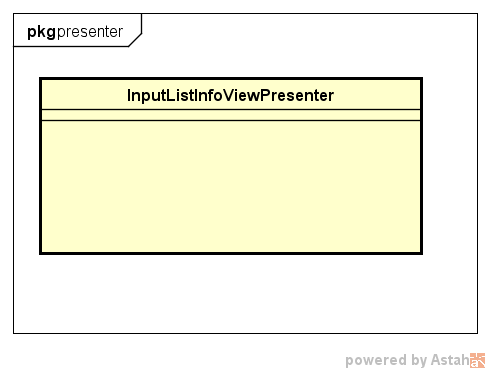
\includegraphics[scale=0.5]{Sezioni/Packages/App/input_list_info_presenter.png}
	\caption{Package application::feature::input\_list\_info::presenter}
\end{figure}
\begin{itemize}
	\item \textbf{Descrizione}: package contenente il presenter per la vista di inserimento dati di una lista
	\item \textbf{Classi e packages contenuti}:
	\begin{itemize}
	\item application::feature::input\_list\_info::presenter::InputListInfoViewPresenter: classe che rappresenta il presenter per la vista di inserimento dati di una lista
	\end{itemize}
\end{itemize}


\subsubsection{Package application::feature::modify\_item}
\label{Package application::feature::modify_item}
\begin{figure}[H]
	\centering
	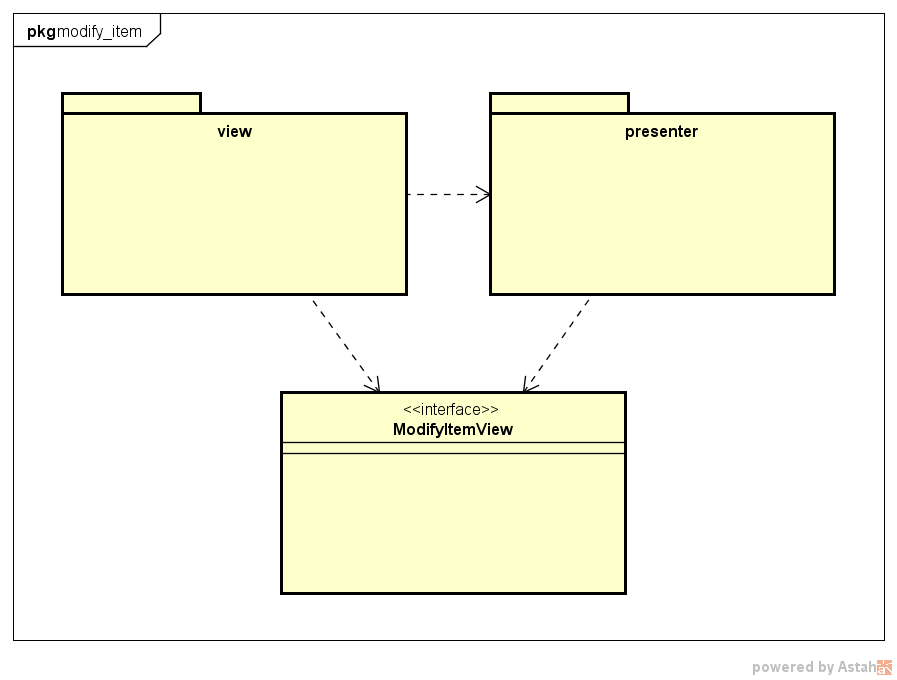
\includegraphics[scale=0.5]{Sezioni/Packages/App/modify_item.png}
	\caption{Package application::feature::modify\_item}
\end{figure}
\begin{itemize}
	\item \textbf{Descrizione}: package contenente i componenti per la funzionalità di modifica di un oggetto all'interno di una lista
	\item \textbf{Classi e packages contenuti}:
	\begin{itemize}
	\item application::feature::modify\_item::view: package contenente la vista per la modifica di un oggetto all'interno di una lista
	\item application::feature::modify\_item::presenter: package contenente il presenter per la vista di modifica di un oggetto all'interno di una lista
	\item application::feature::modify\_item::ModifyItemView: interfaccia rappresentante la vista per la funzionalità modifica di un oggetto all'interno di una lista
	\end{itemize}
\end{itemize}

\subsubsection{Package application::feature::modify\_item::view}
\label{Package application::feature::modify_item::view}
\begin{figure}[H]
	\centering
	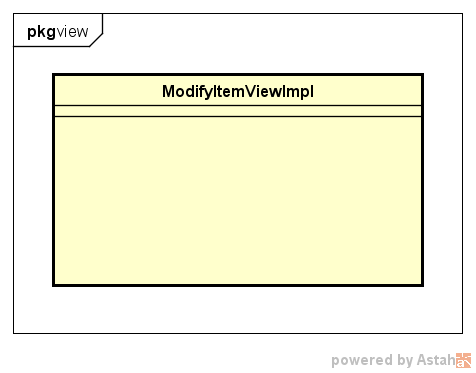
\includegraphics[scale=0.5]{Sezioni/Packages/App/modify_item_view.png}
	\caption{Package application::feature::modify\_item::view}
\end{figure}
\begin{itemize}
	\item \textbf{Descrizione}: package contenente la vista per la funzionalità di modifica di un oggetto all'interno di una lista
	\item \textbf{Classi e packages contenuti}:
	\begin{itemize}
	\item application::feature::modify\_item::view::ModifyItemViewImpl: implementazione dell'interfaccia che rappresenta la vista per la funzionalità di modifica di un oggetto all'interno di una lista
	\end{itemize}
\end{itemize}

\subsubsection{Package application::feature::modify\_item::presenter}
\label{Package application::feature::modify_item::presenter}
\begin{figure}[H]
	\centering
	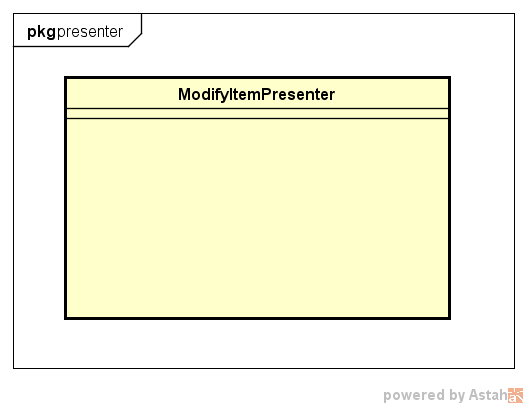
\includegraphics[scale=0.5]{Sezioni/Packages/App/modify_item_presenter.png}
	\caption{Package application::feature::modify\_item::presenter}
\end{figure}
\begin{itemize}
	\item \textbf{Descrizione}: package contenente il presenter per la vista di modifica di un oggetto all'interno di una lista
	\item \textbf{Classi e packages contenuti}:
	\begin{itemize}
	\item application::feature::modify\_item::presenter::ModifyItemViewPresenter: classe che rappresenta il presenter per la vista di modifica di un oggetto all'interno di una lista
	\end{itemize}
\end{itemize}


\subsubsection{Package application::feature::remove\_item}
\label{Package application::feature::remove_item}
\begin{figure}[H]
	\centering
	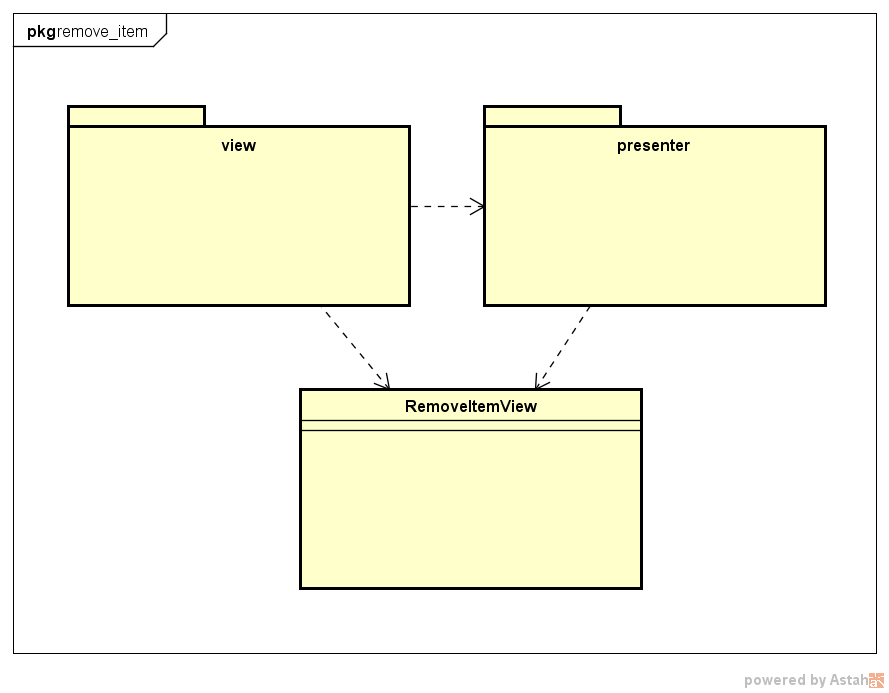
\includegraphics[scale=0.5]{Sezioni/Packages/App/remove_item.png}
	\caption{Package application::feature::remove\_item}
\end{figure}
\begin{itemize}
	\item \textbf{Descrizione}: package contenente i componenti per la funzionalità di rimozione di un oggetto da una lista
	\item \textbf{Classi e packages contenuti}:
	\begin{itemize}
	\item application::feature::remove\_item::view: package contenente la vista per la modifica di un oggetto all'interno di una lista
	\item application::feature::remove\_item::presenter: package contenente il presenter per la vista di modifica di un oggetto all'interno di una lista
	\item application::feature::remove\_item::RemoveItemView: interfaccia rappresentante la vista per la funzionalità modifica di un oggetto all'interno di una lista
	\end{itemize}
\end{itemize}

\subsubsection{Package application::feature::remove\_item::view}
\label{Package application::feature::remove_item::view}
\begin{figure}[H]
	\centering
	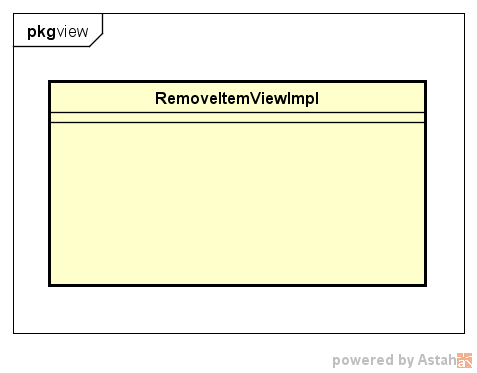
\includegraphics[scale=0.5]{Sezioni/Packages/App/remove_item_view.png}
	\caption{Package application::feature::remove\_item::view}
\end{figure}
\begin{itemize}
	\item \textbf{Descrizione}: package contenente la vista per la funzionalità di rimozione di un oggetto da una lista
	\item \textbf{Classi e packages contenuti}:
	\begin{itemize}
	\item application::feature::remove\_item::view::RemoveItemViewImpl: implementazione dell'interfaccia che rappresenta la vista per la funzionalità di rimozione di un oggetto da una lista
	\end{itemize}
\end{itemize}

\subsubsection{Package application::feature::remove\_item::presenter}
\label{Package application::feature::remove_item::presenter}
\begin{figure}[H]
	\centering
	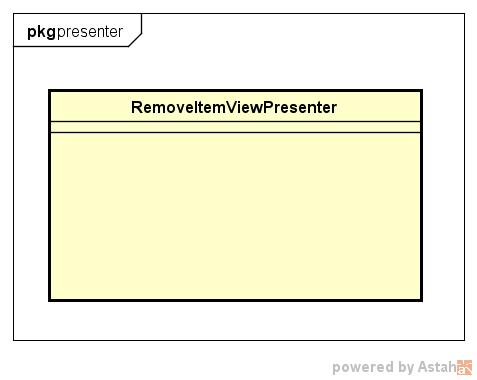
\includegraphics[scale=0.5]{Sezioni/Packages/App/remove_item_presenter.png}
	\caption{Package application::feature::forward::remove\_item::presenter}
\end{figure}
\begin{itemize}
	\item \textbf{Descrizione}: package contenente il presenter per la vista di rimozione di un oggetto da una lista
	\item \textbf{Classi e packages contenuti}:
	\begin{itemize}
	\item application::feature::remove\_item::presenter::RemoveItemViewPresenter: classe che rappresenta il presenter per la vista di rimozione di un oggetto da una lista
	\end{itemize}
\end{itemize}


\subsubsection{Package application::feature::sharewithcontact}
\label{Package application::feature::sharewithcontact}
\begin{figure}[H]
	\centering
	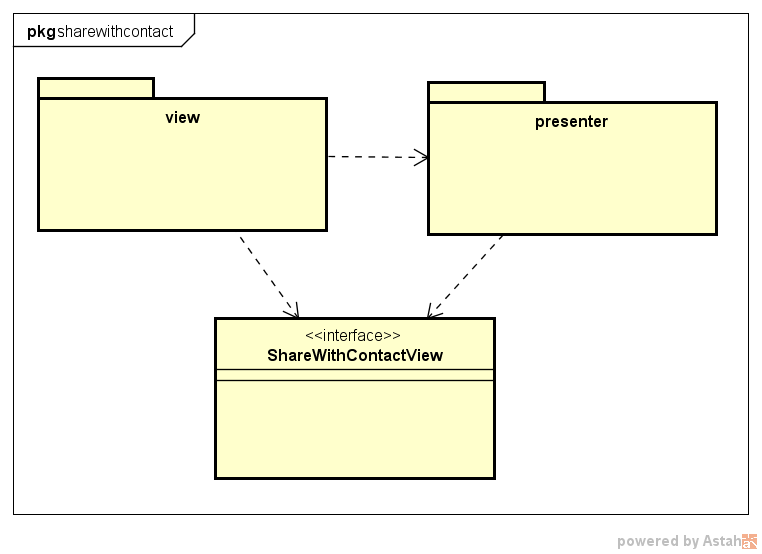
\includegraphics[scale=0.5]{Sezioni/Packages/App/share_with_contact.png}
	\caption{Package application::feature::sharewithcontact}
\end{figure}
\begin{itemize}
	\item \textbf{Descrizione}: package contenente i componenti per la funzionalità di condivisione della lista con un contatto
	\item \textbf{Classi e packages contenuti}:
	\begin{itemize}
	\item application::feature::sharewithcontact::view: package contenente la vista per la modifica di un oggetto all'interno di una lista
	\item application::feature::sharewithcontact::presenter: package contenente il presenter per la vista di modifica di un oggetto all'interno di una lista
	\item application::feature::sharewithcontact::ShareWithContactView: interfaccia rappresentante la vista per la funzionalità modifica di un oggetto all'interno di una lista
	\end{itemize}
\end{itemize}

\subsubsection{Package application::feature::sharewithcontact::view}\label{Package application::feature::sharewithcontact::view}
\begin{figure}[H]
	\centering
	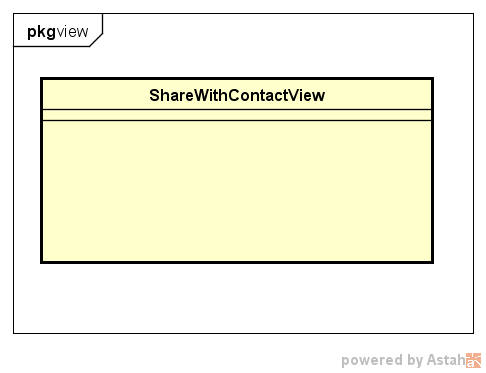
\includegraphics[scale=0.5]{Sezioni/Packages/App/share_with_contact_view.png}
	\caption{Package application::feature::sharewithcontact::view}
\end{figure}
\begin{itemize}
	\item \textbf{Descrizione}: package contenente la vista per la funzionalità di condivisione della lista con un contatto
	\item \textbf{Classi e packages contenuti}:
	\begin{itemize}
	\item application::feature::sharewithcontact::view::ShareWithContactViewImpl: implementazione dell'interfaccia che rappresenta la vista per la funzionalità di condivisione della lista con un contatto
	\end{itemize}
\end{itemize}

\subsubsection{Package application::feature::sharewithcontact::presenter}
\label{Package application::feature::sharewithcontact::presenter}
\begin{figure}[H]
	\centering
	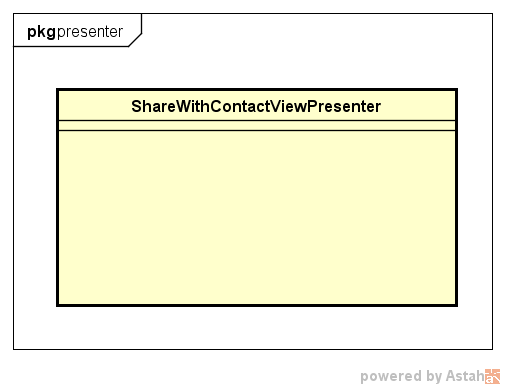
\includegraphics[scale=0.5]{Sezioni/Packages/App/share_with_contact_presenter.png}
	\caption{Package application::feature::sharewithcontact::presenter}
\end{figure}
\begin{itemize}
	\item \textbf{Descrizione}: package contenente il presenter per la vista di condivisione della lista con un contatto
	\item \textbf{Classi e packages contenuti}:
	\begin{itemize}
	\item application::feature::sharewithcontact::presenter::ShareWithContactViewPresenter: classe che rappresenta il presenter per la vista di condivisione della lista con un contatto
	\end{itemize}
\end{itemize}


\subsubsection{Package application::feature::sharewithgroup}
\label{Package application::feature::sharewithgroup}
\begin{figure}[H]
	\centering
	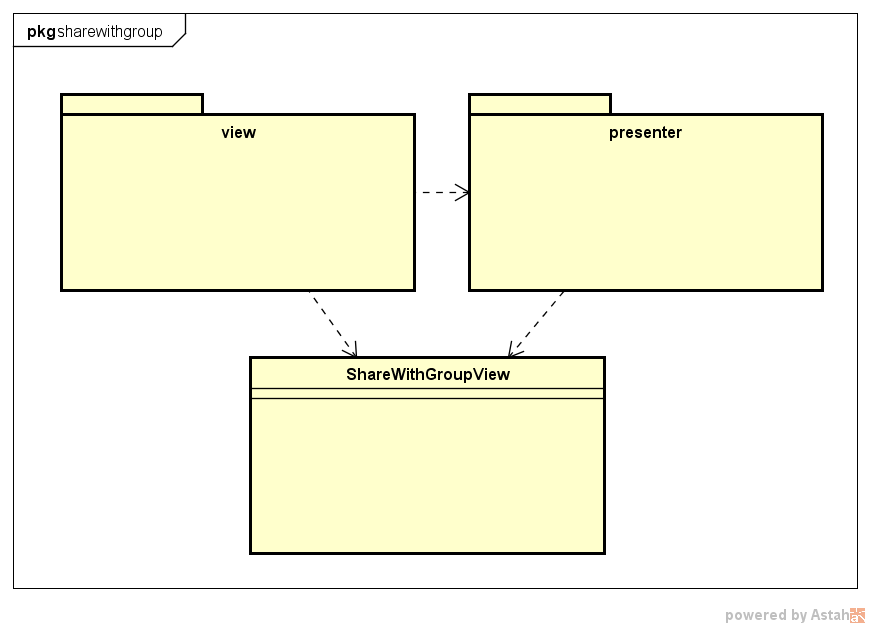
\includegraphics[scale=0.5]{Sezioni/Packages/App/share_with_group.png}
	\caption{Package application::feature::sharewithgroup}
\end{figure}
\begin{itemize}
	\item \textbf{Descrizione}: package contenente i componenti per la funzionalità di condivisione della lista con un gruppo
	\item \textbf{Classi e packages contenuti}:
	\begin{itemize}
	\item application::feature::sharewithgroup::view: package contenente la vista per la modifica di un oggetto all'interno di una lista
	\item application::feature::sharewithgroup::presenter: package contenente il presenter per la vista di modifica di un oggetto all'interno di una lista
	\item application::feature::sharewithgroup::ShareWithGroupView: interfaccia rappresentante la vista per la funzionalità modifica di un oggetto all'interno di una lista
	\end{itemize}
\end{itemize}

\subsubsection{Package application::feature::sharewithgroup::view}
\label{Package application::feature::sharewithgroup::view}
\begin{figure}[H]
	\centering
	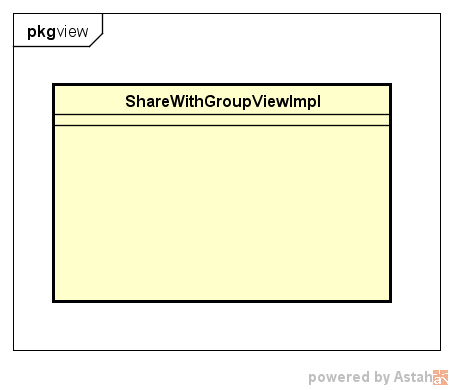
\includegraphics[scale=0.5]{Sezioni/Packages/App/share_with_group_view.png}
	\caption{Package application::feature::sharewithgroup::view}
\end{figure}
\begin{itemize}
	\item \textbf{Descrizione}: package contenente la vista per la funzionalità di condivisione della lista con un gruppo
	\item \textbf{Classi e packages contenuti}:
	\begin{itemize}
	\item application::feature::sharewithgroup::view::ShareWithGroupViewImpl: implementazione dell'interfaccia che rappresenta la vista per la funzionalità di condivisione della lista con un gruppo
	\end{itemize}
\end{itemize}

\subsubsection{Package application::feature::sharewithgroup::presenter}
\label{Package application::feature::sharewithgroup::presenter}
\begin{figure}[H]
	\centering
	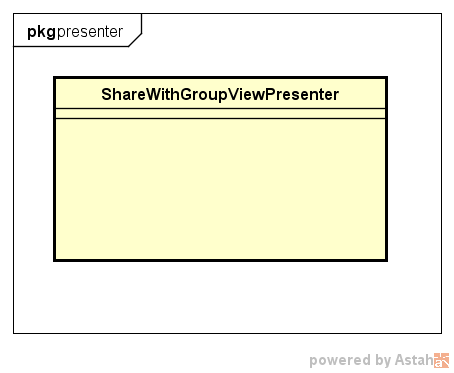
\includegraphics[scale=0.5]{Sezioni/Packages/App/share_with_group_presenter.png}
	\caption{Package application::feature::sharewithgroup::presenter}
\end{figure}
\begin{itemize}
	\item \textbf{Descrizione}: package contenente il presenter per la vista di condivisione della lista con un gruppo
	\item \textbf{Classi e packages contenuti}:
	\begin{itemize}
	\item application::feature::sharewithgroup::presenter::ShareWithGroupViewPresenter: classe che rappresenta il presenter per la vista di condivisione della lista con un gruppo
	\end{itemize}
\end{itemize}


\subsubsection{Package application::feature::help}
\label{Package application::feature::help}
\begin{figure}[H]
	\centering
	\includegraphics[scale=0.5]{Sezioni/Packages/App/help.png}
	\caption{Package application::feature::help}
\end{figure}
\begin{itemize}
	\item \textbf{Descrizione}: package contenente i componenti per la funzionalità di visualizzazione aiuto per l'utilizzo dell'applicazione
	\item \textbf{Classi e packages contenuti}:
	\begin{itemize}
	\item application::feature::help::view: package contenente la vista per la modifica di un oggetto all'interno di una lista
	\item application::feature::help::presenter: package contenente il presenter per la vista di modifica di un oggetto all'interno di una lista
	\item application::feature::help::helpView: interfaccia rappresentante la vista per la funzionalità modifica di un oggetto all'interno di una lista
	\end{itemize}
\end{itemize}

\subsubsection{Package application::feature::help::view}
\label{Package application::feature::help::view}
\begin{figure}[H]
	\centering
	\includegraphics[scale=0.5]{Sezioni/Packages/App/help_view.png}
	\caption{Package application::feature::help::view}
\end{figure}
\begin{itemize}
	\item \textbf{Descrizione}: package contenente la vista per la funzionalità di visualizzazione aiuto per l'utilizzo dell'applicazione
	\item \textbf{Classi e packages contenuti}:
	\begin{itemize}
	\item application::feature::help::view::helpViewImpl: implementazione dell'interfaccia che rappresenta la vista per la funzionalità di visualizzazione aiuto per l'utilizzo dell'applicazione
	\end{itemize}
\end{itemize}

\subsubsection{Package application::feature::help::presenter}
\label{Package application::feature::help::presenter}
\begin{figure}[H]
	\centering
	\includegraphics[scale=0.5]{Sezioni/Packages/App/help_presenter.png}
	\caption{Package application::feature::help::presenter}
\end{figure}
\begin{itemize}
	\item \textbf{Descrizione}: package contenente il presenter per la vista di visualizzazione aiuto per l'utilizzo dell'applicazione
	\item \textbf{Classi e packages contenuti}:
	\begin{itemize}
	\item application::feature::help::presenter::helpViewPresenter: classe che rappresenta il presenter per la vista di visualizzazione aiuto per l'utilizzo dell'applicazione
	\end{itemize}
\end{itemize}

\subsubsection{Package application::feature::exception}
\label{Package application::feature::exception}
\begin{figure}[H]
	\centering
	\includegraphics[scale=0.5]{Sezioni/Packages/App/exception.png}
	\caption{Package application::feature::exception}
\end{figure}
\begin{itemize}
	\item \textbf{Descrizione}: package contenente tutte le eccezioni che l'applicazione può lanciare durante l'esecuzione
	\item \textbf{Classi e packages contenuti}:
	\begin{itemize}
	\item application::feature::exception::Exception: classe che rappresenta una eccezione generica
	\item application::feature::exception::BadParameterException: classe che rappresenta una eccezione lanciata nel qual caso un parametro di un metodo sia incorretto
	\end{itemize}
\end{itemize}


\newpage
\section{Specifica Tecnica}

\subsection{SDK}

\subsubsection{BaseBubble}

\label{BaseBubble}
\begin{figure}[ht]
	\centering
	\includegraphics[scale=0.5]{Sezioni/SottosezioniST/img/BaseBubble.png}
	\caption{BaseBubble}
\end{figure}

\begin{itemize}
\item \textbf{Descrizione:} Classe base astratta che rappresenta le bolle di Monolith.
\item \textbf{Utilizzo:} Classe base astratta utilizzata ed estesa ogni qualvolta uno sviluppatore intende creare nuove bolle.
\item \textbf{Attributi:} 
\begin{itemize}
\item \textit{protected layout:VerticalLayoutView}\\
Oggetto che rappresenta il layout verticale della bolla.
\end{itemize}
\item \textbf{Metodi:}
\begin{itemize}
\item \textit{public addComponent(component:BaseComponent):void}\\
Aggiunge un widget alla bolla.
\item{\textbf{Parametri}: \begin{itemize}
\item \textit{component:BaseComponent}\\
Oggetto che rappresenta il componente che si desidera aggiungere alla bolla.
\end{itemize}}
\item \textit{public renderView():string}\\
Genera il codice HTML, CSS e JavaScript necessario per visualizzare bolle.
\end{itemize}
\end{itemize}

\subsubsection{ToDoListBubble}

\label{ToDoListBubble}
\begin{figure}[ht]
	\centering
	\includegraphics[scale=0.5]{Sezioni/SottosezioniST/img/ToDoListBubble.png}
	\caption{ToDoListBubble}
\end{figure}

\begin{itemize}
\item \textbf{Descrizione:} Classe concreta che estende BaseBubble, destinata alla creazione di bolle lista di Monolith.
\item \textbf{Utilizzo:} Classe utilizzata ogni qualvolta uno sviluppatore intende creare nuove bolle lista.
\item \textbf{Attributi:}
\begin{itemize}
\item \textit{private textView:TextWidgetView}\\
Oggetto che rappresenta il widget contenente il testo della bolla lista.
\item \textit{private checklist:CheckListView}\\
Oggetto che rappresenta il widget contenente la lista di oggetti che si possono spuntare.
\end{itemize}
\item \textbf{Metodi:}
\begin{itemize}
\item \textit{public ToDoListBubble():ToDoListBubble}\\
Il costruttore della classe ToDoListBubble.
\item \textit{public addItem(item:string):void}\\
Aggiunge un elemento con il nome definito alla bolla lista.
\item{\textbf{Parametri}: \begin{itemize}
\item \textit{item:string}\\
Valore che rappresenta il nome dell'elemento che si vuole aggiungere alla lista.
\end{itemize}}
\end{itemize}
\end{itemize}

\subsubsection{MarkdownBubble}

\label{MarkdownBubble}
\begin{figure}[ht]
	\centering
	\includegraphics[scale=0.5]{Sezioni/SottosezioniST/img/MarkdownBubble.png}
	\caption{MarkDownBubble}
\end{figure}

\begin{itemize}
\item \textbf{Descrizione:} Classe concreta che estende BaseBubble, destinata alla creazione di bolle testo markdown di Monolith.
\item \textbf{Utilizzo:} Classe utilizzata ogni qualvolta uno sviluppatore intende creare nuove bolle testo markdown.
\item \textbf{Attributi:}
\begin{itemize}
\item \textit{private textview:TextWidgetView}\\
Oggetto che rappresenta il widget contenente il testo della bolla testo markdown.
\end{itemize}
\item \textbf{Metodi:}
\begin{itemize}
\item \textit{public MarkdownBubble():MarkdownBubble}\\
Il costruttore della classe MarkdownBubble.
\item \textit{public setText(text:string):void}\\
Imposta il testo della bolla lista con il valore definito.
\item{\textbf{Parametri}: \begin{itemize}
\item \textit{text:string}\\
Valore che rappresenta il testo che si vuole inserire nella bolla testo markdown.
\end{itemize}}
\end{itemize}
\end{itemize}

\subsubsection{AlertBubble}

\label{AlertBubble}
\begin{figure}[ht]
	\centering
	\includegraphics[scale=0.5]{Sezioni/SottosezioniST/img/AlertBubble.png}
	\caption{AlertBubble}
\end{figure}

\begin{itemize}
\item \textbf{Descrizione:} Classe concreta che estende BaseBubble, destinata alla creazione di bolle avviso di Monolith.
\item \textbf{Utilizzo:} Classe utilizzata ogni qualvolta uno sviluppatore intende creare nuove bolle avviso.
\item \textbf{Attributi:} 
\begin{itemize}
\item \textit{private titleView:TextWidgetView}\\
Campo che rappresenta e contiene il titolo della bolla avviso.
\item \textit{private messageView:TextWidgetView}\\
Campo che rappresenta e contiene il messaggio della bolla avviso.
\end{itemize}
\item \textbf{Metodi:}
\begin{itemize}
\item \textit{public AlertBubble():AlertBubble}\\
Il costruttore della classe AlertBubble.
\item \textit{public setTitle(title:string):void}\\
Imposta il titolo della bolla avviso con il valore title.
\item{\textbf{Parametri}: \begin{itemize}
\item \textit{title:string}\\
Valore che rappresenta il titolo che si vuole impostare alla bolla avviso.
\end{itemize}}
\item \textit{public setMessage(message:string):void}\\
Imposta il messaggio della bolla avviso con il valore message.
\item{\textbf{Parametri}: \begin{itemize}
\item \textit{message:string}\\
Valore che rappresenta il messaggio testuale che si vuole impostare alla bolla avviso.
\end{itemize}}
\end{itemize}
\end{itemize}
\subsubsection{BaseComponent}

\label{BaseComponent}
\begin{figure}[ht]
	\centering
	\includegraphics[scale=0.5]{Sezioni/SottosezioniST/img/BaseComponent.png}
	\caption{BaseComponent}
\end{figure}

\begin{itemize}
\item \textbf{Descrizione:} Interfaccia base che rappresenta un qualsiasi oggetto che può essere inserito all'interno di un bolla.
\item \textbf{Utilizzo:} Interfaccia che viene implementata ogni qualvolta uno sviluppatore intende inserire all'interno di un bolla un widget o un layout.
\item \textbf{Attributi:}
\item \textbf{Metodi:}
\begin{itemize}
\item \textit{public renderView():string}\\
Genera il codice HTML, CSS e JavaScript necessario per visualizzare BaseComponent.
\end{itemize}
\end{itemize}
\subsubsection{monolith::client::component::layout::BaseLayout}

\label{monolith::client::component::layout::BaseLayout}
\begin{figure}[ht]
	\centering
	\includegraphics[scale=0.5]{Sezioni/SottosezioniST/img/BaseLayout.png}
	\caption{monolith::client::component::layout::BaseLayout}
\end{figure}

\begin{itemize}
\item \textbf{Descrizione:} Classe astratta che implementa l'interfaccia BaseComponent e che rappresenta un oggetto layout per la disposizione di componenti nelle bolle di Monolith.
\item \textbf{Utilizzo:} Classe utilizzata ed estesa ogni qualvolta uno sviluppatore intende creare un nuovo layout da inserire in una bolla.
\item \textbf{Attributi:}
\begin{itemize}
\item \textit{private items:List<BaseComponent>}\\
Rappresenta la lista di oggetti BaseComponent contenuti nel layout.
\end{itemize}
\item \textbf{Metodi:}
\begin{itemize}
\item \textit{public addItem(component:BaseComponent):void}\\
Aggiunge un oggetto BaseComponent al layout.
\\ \textbf{Parametri}: \begin{itemize}
\item \textit{component:BaseComponent}\\
Oggetto che rappresenta il BaseComponent da aggiungere al layout.
\end{itemize}
\end{itemize}
\end{itemize}

\subsubsection{monolith::client::component::layout::vertical::VerticalLayoutView}

\label{monolith::client::component::layout::vertical::VerticalLayoutView}
\begin{figure}[H]
	\centering
	\includegraphics[scale=0.5]{Sezioni/SottosezioniST/img/VerticalLayoutView.png}
	\caption{monolith::client::component::layout::vertical::VerticalLayoutView}
\end{figure}

\begin{itemize}
\item \textbf{Descrizione:} Classe concreta che estende BaseLayout, destinata alla creazione di layout per la disposizione verticale di BaseComponent.
\item \textbf{Utilizzo:} Classe utilizzata ogni qualvolta uno sviluppatore intende creare un nuovo layout orizzontale da inserire in una bolla.
\item \textbf{Attributi:}
\item \textbf{Metodi:}
\begin{itemize}
\item\textit{public VerticalLayoutView():VerticalLayoutView}\\
Il costruttore per la classe VerticalLayoutView.
\item \textit{public addItem(component:BaseComponent):void}\\
Aggiunge un oggetto BaseComponent al layout verticale.
\\ \textbf{Parametri}: \begin{itemize}
\item \textit{component:BaseComponent}\\
Oggetto che rappresenta il BaseComponent da aggiungere al layout verticale.
\end{itemize}
\item \textit{public renderView():HtmlDOMElement}\\
Restituisce l'elemento DOM rappresentante i BaseComponent disposti nel layout verticale.
\end{itemize}
\end{itemize}

\subsubsection{monolith::client::component::layout::horizontal::HorizontalLayoutView}

\label{monolith::client::component::layout::horizontal::HorizontalLayoutView}
\begin{figure}[H]
	\centering
	\includegraphics[scale=0.5]{Sezioni/SottosezioniST/img/HorizontalLayoutView.png}
	\caption{monolith::client::component::layout::horizontal::HorizontalLayoutView}
\end{figure}

\begin{itemize}
\item \textbf{Descrizione:} Classe concreta che estende BaseLayout, destinata alla creazione di layout  per la disposizione orizzontale di BaseComponent.
\item \textbf{Utilizzo:} Classe utilizzata ogni qualvolta uno sviluppatore intende creare un nuovo layout verticale da inserire in una bolla.
\item \textbf{Attributi:}
\item \textbf{Metodi:}
\begin{itemize}
\item\textit{public HorizontalLayoutView():HorizontalLayoutView}\\
Il costruttore per la classe HorizontalLayoutView.
\item \textit{private createColumn():Object}\\
Crea una colonna per la disposizione degli oggetti in senso orizzontale del layout
\item \textit{public addItem(component:BaseComponent):void}\\
Aggiunge un oggetto BaseComponent al layout orizzontale.
\\ \textbf{Parametri}: \begin{itemize}
\item \textit{component:BaseComponent}\\
Oggetto che rappresenta il BaseComponent da aggiungere al layout orizzontale.
\end{itemize}
\item \textit{public renderView():HtmlDOMElement}\\
Restituisce l'elemento DOM rappresentante i BaseComponent disposti nel layout orizzontale.
\end{itemize}
\end{itemize}
\subsection{Widgets}
\subsubsection{TextWidget}
\begin{lstlisting}[language=JavaScript]
// Create a TextWidget
let textWidget = new Monolith.Widget.TextWidget;

// Hide the widget
textWidget.setVisibility(false); // Default is true, which will show is

// Set the text. Markdown notation is also supported
textWidget.setText("Foo");
textWidget.setText("Markdown __is supported__ **too**");

// Set the text color using HEX notation (http://www.color-hex.com/)
textWidget.setTextColor("#C61A10");

// Set the text size in pixel
textWidget.setTextSize(15);

// Set the URL highlighting color
textWidget.setUrlHighligthColor("#EE42F4");

// Enable or disable the text formatting, this includes also URL highlighting
textWidget.setFormatText(true);
textWidget.setFormatText(false);
\end{lstlisting}
~\\~\\

\subsubsection{ImageWidget}
\begin{lstlisting}[language=JavaScript]
// Create the ImageWidget
let imageWidget = new Monolith.Widget.ImageWidget;

// Hide the widget
imageWidget.setVisibility(false); // Default is true, which will show is

// Set the image associated with the widget
imageWidget.setImage("path/to/image.png");

// Set the image dimensions
imageWidget.setWidth(200);
imageWidget.setHeight(50);
\end{lstlisting}

\newpage
\subsubsection{ButtonWidget}
\begin{lstlisting}[language=JavaScript]
// Create a ButtonWidget
let buttonWidget = new Monolith.Widget.ButtonWidget;

// Set the dimensions of the button
buttonWidget.setWidth(100);
buttonWidget.setHeight(50);

// Set the color of the button
buttonWidget.setBackgroundColor("#41F492");

// Set the action associated with the button
buttonWidget.setOnClickAction(function(){
    alert("The button has been clicked");
});

// Set the action associated with the button when the user long-clicks it
buttonWidget.setOnLongClickAction(function(){
    alert("The button has been long clicked");
});

// Set the milliseconds that need to pass before a click is considered a long click
buttonWidget.setOnLongClickActionTimer(500);
\end{lstlisting}
~\\~\\

\subsubsection{ListWidget}
\begin{lstlisting}[language=JavaScript]
// Create the ListWidget
let listWidget = new Monolith.Widget.ListWidget;

// Add items to the list
listWidget.addItem("First");
listWidget.addItem("Second");
listWidget.addItem("Third");

// Set the indicator of the list
listWidget.setCharacterNumber(); // Numbered list
listWidget.setCharacterCircle(); // Unnumbered list

// Set the indicator color
listWidget. setColor("#292929");
\end{lstlisting}

\newpage
\subsubsection{CheckListItemWidget}
\begin{lstlisting}[language=JavaScript]
// Create a new CheckListItemWidget
let checkListItemWidget = new Monolith.Widget.CheckListItemWidget;

// Set the text associated with the item
checkListItemWidget.setText("Click me!");

// Customize the check appereance
// Color the check box instead of using a check tick
checkListItemWidget.setUseSelectionMark(true); 
// Set the color that will be used to color the check box
checkListItemWidget.setSelectionColor("#AAAAAA"); 
// Use a check tick
checkListItemWidget.setUseSelectionMark(false); 
// Set the character used as check tick
checkListItemWidget.setSelectionCharacter("X"); 

// Check or un-check the option
checkListItemWidget.setChecked(true); // Checked
checkListItemWidget.setChecked(false); // Un-checked

// Know it the option is checked or not
let isChecked = checkListItemWidget.isChecked();
if (isChecked){
    // The option is checked
} else {
    // The option is not checked
}


// Set the action to perform on click
checkListItemWidget.setOnClick(function(item){
    // The item parameter represents the view of the item that has been clicked
    item.setText("New text after click");
});

// Set the action to perform after a long click (1000 ms)
checkListItemWidget.setOnLongClick(function(){
    // The item parameter represents the view of the item that has been clicked
   item.setText("New text after long click");
});


// Delete the item
checkListItemWidget.removeOption();
\end{lstlisting}

\newpage
\subsubsection{Create a custom widget}
In order to create a new custom widget and add it to \termine{Monolith} so than you can use it like the default ones, you have to do as follows.
\begin{enumerate}

	\item Create a new class which extends from \texttt{BaseWidget}
\begin{lstlisting}[language=JavaScript]
export class MyWidget extends Monolith.Widget.BaseWidget {

    constructor(){
        super(); // You need to call this to create the above hierarchy
        
        // Initialize your widget here
    }
    
    renderView(){
        // Renders the view of the widget and returns a DOMElement object
    }

    performOperation(){
        // Perform some operation
    }

}
\end{lstlisting}

	\item Use your widget wherever you want
\begin{lstlisting}[language=JavaScript]
// Import the widget
import {MyWidget} from '/path/to/MyWidget.js';

// Istantiate the widget
let myWidget = new MyWidget();

// Perform operations with the widget
myWidget.performOperation();

// Render the widget's view
myWidget.renderView();
\end{lstlisting}
  
\end{enumerate}  
  
\textbf{Note} \\ 
The default widget's behaviour does \textbf{not} let the user use a single widget without a bubble container that holds it. \\
If you plan to render the widget's view inside a Rocket.chat room, please create a bubble and add your widget to the bubble, so that the bubble will render it and show it to the user.

\newpage



\subsection{Applicazione demo lista-spesa}

\newpage
\newpage
\section{Diagrammi di Sequenza}
\subsection{SDK}

\subsubsection{Creazione di un widget immagine}

\label{Creazione di un widget immagine}
\begin{figure}[ht]
	\centering
	\includegraphics[width=16cm, height=14cm]{Sezioni/Diagrammi/img/Creazione di un widget immagine.png}
	\caption{Creazione di un widget immagine}
\end{figure}

Lo sviluppatore può creare un widget di tipo immagine per aggiungerlo ad una sua ipotetica \termine{bolla}. Durante la costruzione, come si vede dallo schema, vengono invocati tre metodi. Il primo per impostare l'immagine e gli altri due per impostare rispettivamente la larghezza ed altezza di essa. Il tipo delle immagini supportate sono le stesse supportate da \termine{Rocket.Chat} ovvero:
\begin{itemize}
\item .jpeg
\item .gif
\item .png
\item .jpg
\end{itemize}
Se l'immagine inserita non appartiene ad uno di questi formati oppure non viene inserita dallo sviluppatore il metodo \texttt{setText} di \texttt{TextWidgetPresenter} lancerà un'eccezione di tipo \texttt{BadParameterException}. \\
Le frecce di ritorno dall'\texttt{ImageWidgetPresenter} all'\texttt{ImageWidget} sono state inserite poiché il cambiamento dei dati sul \termine{Presenter} ha effetto anche sulla View. La comunicazione tra queste due unità avviene tramite il \termine{framework} \termine{vue.js}. \\
Si noti, infine, che i metodi invocati da \texttt{ImageWidget} vengono chiamati in quest'ordine dal suo costruttore senza parametri. Tali metodi possono anche essere chiamati singolarmente dallo sviluppatore secondo l'ordine che egli preferisce. Queste azioni non verranno ulteriormente descritte poiché ritenute ridondanti.

\newpage

\subsubsection{Creazione di un widget di testo}

\label{Creazione di un widget di testo}
\begin{figure}[H]
	\centering
	\includegraphics[width=16cm, height=14cm]{Sezioni/Diagrammi/img/Creazione di un widget di testo.png}
	\caption{Creazione di un widget di testo}
\end{figure}

Lo sviluppatore può creare un widget di tipo testo per aggiungerlo ad una sua ipotetica \termine{bolla}. Affinché non si verifichino errori il testo inserito nel widget deve essere valido, ovvero non deve contenere caratteri speciali se non quelli supportati dal tipo di codifica UTF-8 e non deve essere del testo vuoto. Se ciò dovesse capitare il metodo \texttt{setText} di \texttt{TextWidgetPresenter} lancerà un'eccezione di tipo \texttt{BadParameterException}. \\
Le frecce di ritorno dal \texttt{TextWidgetPresenter}  al \texttt{TextWidget} sono state inserite poiché il cambiamento dei dati sul \termine{Presenter} ha effetto anche sulla View. La comunicazione tra queste due unità avviene tramite il \termine{framework} \termine{vue.js}. \\
Si noti, infine, che i metodi invocati da \texttt{TextWidget} vengono chiamati in quest'ordine dal suo costruttore senza parametri. Tali metodi possono anche essere chiamati singolarmente dallo sviluppatore secondo l'ordine che egli preferisce. Queste azioni non verranno ulteriormente descritte poiché ritenute ridondanti.

\newpage

\subsubsection{Creazione di un widget Checklist}

\label{Creazione di un widget Checklist}
\begin{figure}[H]
	\centering
	\includegraphics[width=16cm, height=14cm]{Sezioni/Diagrammi/img/Creazione di un widget CheckList.png}
	\caption{Creazione di un widget Checklist}
\end{figure}

Lo sviluppatore può creare un widget di tipo Checklist per aggiungerlo ad una sua ipotetica \termine{bolla}. Affinché non si verifichino errori, quando si usa il metodo \texttt{setSelectionCharacter} deve essere inserito correttamente un carattere per la spunta supportato. Inoltre se il flag \texttt{useSelectionMark} è stato impostato a false allora, indipendentemente dal carattere scelto dalla spunta, verrà usato il colore.\\
Le frecce di ritorno dal \texttt{ChecklistWidgetPresenter}  al \texttt{ChecklistWidget} sono state inserite poiché il cambiamento dei dati sul \termine{Presenter} ha effetto anche sulla View. La comunicazione tra queste due unità avviene tramite il \termine{framework} \termine{vue.js}. \\
Si noti, infine, che i metodi invocati da \texttt{Checklist} vengono chiamati in quest'ordine dal suo costruttore senza parametri. Tali metodi possono anche essere chiamati singolarmente dallo sviluppatore secondo l'ordine che egli preferisce. Queste azioni non verranno ulteriormente descritte poiché ritenute ridondanti.

\newpage

\subsubsection{Aggiungere un messaggio di completamento al widget Checklist}

\label{Aggiungere un messaggio di completamento al widget Checklist}
\begin{figure}[H]
	\centering
	\includegraphics[width=16cm, height=14cm]{Sezioni/Diagrammi/img/Aggiungere un messaggio di completamento al widget Checklist.png}
	\caption{Aggiungere un messaggio di completamento al widget Checklist}
\end{figure}

Lo sviluppatore può aggiungere un messaggio di completamento per il widget Checklist. Questo messaggio verrà visualizzato non appena tutte le entry del widget saranno spuntate, ovvero al lancio dell'evento \texttt{emitOnCompletedList}.

\newpage

\subsubsection{Creazione di un widget bottone}

\label{Creazione di un widget bottone}
\begin{figure}[H]
	\centering
	\includegraphics[width=16cm, height=14cm]{Sezioni/Diagrammi/img/Creazione di un widget bottone.png}
	\caption{Creazione di un widget bottone}
\end{figure}

Lo sviluppatore può creare un widget di tipo bottone per aggiungerlo ad una sua ipotetica \termine{bolla}. Se, durante la creazione del widget, il testo non dovesse essere impostato correttamente, il metodo \texttt{setText} di \texttt{ButtonWidgetPresenter} lancerà un'eccezione di tipo \texttt{BadParameterException}. \\
Le frecce di ritorno da \texttt{ButtonWidgetPresenter}  a \texttt{ButtonWidget} sono state inserite poiché il cambiamento dei dati sul \termine{Presenter} ha effetto anche sulla View. La comunicazione tra queste due unità avviene tramite il \termine{framework} \termine{vue.js}. \\
Si noti, infine, che i metodi invocati da \texttt{ButtonWidget} vengono chiamati in quest'ordine dal suo costruttore senza parametri. Tali metodi possono anche essere chiamati singolarmente dallo sviluppatore secondo l'ordine che egli preferisce. Queste azioni non verranno ulteriormente descritte poiché ritenute ridondanti.

\newpage

\subsubsection{Creazione di un listWidget}

\label{Click di un bottone}
\begin{figure}[H]
	\centering
	\includegraphics[width=16cm, height=14cm]{Sezioni/Diagrammi/img/Creazione di un listWidget.png}
	\caption{Creazione di un listWidget}
\end{figure}

Lo sviluppatore può creare un widget di tipo lista per aggiungerlo ad una sua ipotetica \termine{bolla}. Ogni elemento aggiunto logicamente dal presenter agisce anche sulla view. Per questo tipo di comunicazione si rimanda al \termine{framework} \termine{vue.js}. \\
L'azione compiuta per creare il widget può essere anche effettuata a posteriori della creazione del widget, questa però, essendo molto simile a quella appena descritta, viene omessa per ridondanza.

\newpage

\subsubsection{Creazione di una bolla aggiungendo un widget checklist}

\label{Creazione di una bolla aggiungendo un widget checklist}
\begin{figure}[H]
	\centering
	\includegraphics[width=16cm, height=14cm]{Sezioni/Diagrammi/img/Creazione di una bolla aggiungendo un widget checklist.png}
	\caption{Creazione di una bolla aggiungendo un widget checklist}
\end{figure}

Lo sviluppatore può aggiungere un widget alla \termine{bolla} appena creata. L'aggiunta dell'elemento avviene tramite il metodo \texttt{addComponent} che permette l'aggiunta sia di un layout che di un widget. Si noti che l'esempio è fatto con un widget specifico, ovvero il widget checklist, ma ciò vale per qualsiasi widget presente nell'\termine{SDK}. Gli altri esempi simili vengono, per questo motivo, omessi.

\newpage

\subsubsection{Aggiunta ad una bolla di un Layout contenente due widget di testo}

\label{Aggiunta ad una bolla di un Layout contenente due widget di testo}
\begin{figure}[H]
	\centering
	\includegraphics[width=16cm, height=14cm]{Sezioni/Diagrammi/img/Aggiunta ad una bolla un Layout contenente due widget di testo.png}
	\caption{Aggiunta ad una bolla di un Layout contenente due widget di testo}
	
\end{figure}
Lo sviluppatore può aggiungere un layout contenente dei widgets alla \termine{bolla}. Anche questo rappresenta solo un generico esempio di come si possa aggiungere un layout ad una \termine{bolla}. Gli altri esempi simili saranno dunque omessi. 

\newpage

\subsubsection{Creazione di una bolla MarkDownBubble}

\label{Creazione di una bolla MarkDownBubble}
\begin{figure}[H]
	\centering
	\includegraphics[width=12cm, height=8cm]{Sezioni/Diagrammi/img/Creazione di una bolla MarkDownBubble.png}
	\caption{Creazione di una bolla MarkDownBubble}
	
\end{figure}

Lo sviluppatore può creare una \termine{bolla} MarkDownBubble disponibile nell'\termine{SDK}.

\subsubsection{Creazione di una bolla AlertBubble}

\label{Creazione di una bolla AlertBubble}
\begin{figure}[H]
	\centering
	\includegraphics[width=12cm, height=8cm]{Sezioni/Diagrammi/img/Creazione di una bolla AlertBubble.png}
	\caption{Creazione di una bolla AlertBubble}
	
\end{figure}

Lo sviluppatore può creare una \termine{bolla} AlertBubble disponibile nell'\termine{SDK}.

\newpage

\subsubsection{Creazione di una bolla ToDoListBubble}

\label{Creazione di una bolla ToDoListBubble}
\begin{figure}[H]
	\centering
	\includegraphics[width=12cm, height=8cm]{Sezioni/Diagrammi/img/Creazione di una bolla ToDoListBubble.png}
	\caption{Creazione di una bolla ToDoListBubble}
	
\end{figure}

Lo sviluppatore può creare una \termine{bolla} ToDoListBubble disponibile nell'\termine{SDK}.



\subsection{Applicazione}
In questi scenari faremo largo uso della libreria\termine{ vue.js} per aggiornare le visualizzazioni, all'interno della chat, delle bolle lista modificate. Lo schema di attivazione è abbastanza semplice in quanto una volta passati al presenter della bolla lista i dati modificati, la libreria \termine {vue.js} si occuperà del aggiornamento in tutte le chat che dipendono dalla lista modificata.
\subsubsection{Creazione di una lista}

\label{Creazione di una lista}
\begin{figure}[ht]
	\centering
	\includegraphics[width=16cm, height=14cm]{Sezioni/Diagrammi/img/Creazione di un widget immagine.png}
	\caption{Creazione di una lista}
\end{figure}

Questo scenario rappresenta l'utente che vuole creare una nuova lista nella chat di \termine{rocket.chat}. Inanzitutto alla pressione del pulsante creazione lista verrà emesso un evento che verrà catturato dalla classe \textit{CreateListVIewImpl} che demanderà la gestione di esso al presenter. Quest'ultimo attraverso il metodo \textit{showInputListInfoView} recupererà il codice html relativo al inserimento dei dati per la creazione della lista e lo mostrerà al utente attraverso un popup creato appositamente dalla chat. Dopo aver finito di inerire i dati desiderati l'utente premerà il relativo pulsante di salvataggio. In questo modo verrà emesso l'evento di salvataggio che verrà gestito dal presenter di \textit{showInputListInfoView} e infine attraverso il metodo \textit{createList} la lista verrà creata nel \termine{database} insieme al id del creatore 



\subsubsection{Cancellazione di una lista}

\label{Cancellazione di una lista}
\begin{figure}[ht]
	\centering
	\includegraphics[width=16cm, height=14cm]{Sezioni/Diagrammi/img/Creazione di un widget CheckList.png}
	\caption{Cancellazione di una lista}
\end{figure}

In questo scenario lo sviluppatore vuole cancellare la propria lista causando l'eliminazione da tutte le chat che la contengono. L'utente quando premerà il bottone elimina lista emetterà un evento che verrà successivamente catturato dalla classe \textit{deleteListViewImpl} che si occuperà di eliminare dal database la lista desiderata attraverso il suo \textit{presenter}. All'avvenuta eliminazione della lista nel \termine{database} verrà emesso l'evento che attiverà i metodi nel presenter della bolla lista per aggiornare, in questo caso eliminare definitivamente,tutte le chat contenti l'istanza di quella lista. 

\subsubsection{Modifica di una lista}

\label{Modifca di un lista}
\begin{figure}[ht]
	\centering
	\includegraphics[width=16cm, height=14cm]{Sezioni/Diagrammi/img/Aggiungere un messaggio di completamento al widget Checklist.png}
	\caption{Modifica di una lista}
\end{figure}

In questo scenario lo sviluppatore vuole modifcare una lista cambiando, ad esempio, il suo nome o l'immagine ad essa associata. L'utente premendo il bottone modifica lista attiverà l'emissione di un evento che verrà catturato dalla classe \textit{ChangeListViewImpl} e demanderà la  gestione al suo presenter. Quest'ultimo attraverso il suo  metodo \textit{showInputListView} gli ritornerà l'html per la modifica della lista completa di tutte le informazioni di essa presenti nel \termine{database}. Successivamente richiamando il metodo \textit{showPopUp} si visualizzerà a schermo  le informazioni prima ottenute con la possibilità di modificarle. Una volta modificate le informazioni desiderate l'utente premerà il pulsante di conferma modifica in questo modo verrà emmesso l'evento di salvataggio che verrà catturato dalla classe \textit{InpuListInfoViewImpl} e successivamente demandato alla classe \textit{ChangeListPresenter} che si occuperà di salvare le modifiche nel \termine{database}.
All'avvenuta modifica della lista  verrà emesso l'evento che attiverà i metodi nel presenter della bolla lista per aggiornare tutte le chat contenti l'istanza di quella lista.
 
\subsubsection{Iterazione con lista [RICCARDO MONTAGNIN}

RICCARDO MONTAGNIN


\subsubsection{Aggiunta di un Item}

\label{Aggiunta di un Item}
\begin{figure}[ht]
	\centering
	\includegraphics[width=16cm, height=14cm]{Sezioni/Diagrammi/img/Creazione di un widget bottone.png}
	\caption{Aggiunta di un Item}
\end{figure}

In questo scenario lo sviluppatore vuole aggiungere dei prodotti (chiamati \termine{item} nella nostra applicazione} alla lista da esso creata. Oppure vuole aggiungerli a una lista nella quale ha permessi di modifca. L'utente premendo il pulsante \textit{aggiungi item} farà emettere un evento che verrà catturato dalla classe \textit{AddItemViewImpl} che demanderà la gestione al suo presenter. Quest'ultimo attraverso il metodo \textit{showInputInfoView} recupererà l'html necessario per la corretta aggiunta di un item e successivamente attraverso la classe \textit{showPopUpUseCase} farà visualizzare a schermo le informazioni prima recuperate. L'utente una volta che ha inserito le informazioni desiderate premerà il pulsante di aggiunta del item. In questo modo verrà emesso l'evento di salvataggio che verrà poi catturato dalla classe \textit{InputItemInfoViewImpl} che si occuperà di creare l'item ed emettere un evento per l'avvenuta creazione ed infine la classe \textit{AddItemViewPresenter} si occuperà di memorizzare la  lista con il nuovo \termine{item} nel \termine{database}. Infine all'avvenuta modifca della lista nel \termine{database} verrano eseguiti i metodi nel presenter della bolla lista per aggiornare tutti le chat contenenti l'istanza della lista appena modificata. 




\subsubsection{Modifica Item}

\label{Modifica Item}
\begin{figure}[ht]
	\centering
	\includegraphics[width=16cm, height=14cm]{Sezioni/Diagrammi/img/Creazione di una bolla aggiungendo un widget checklist.png}
	\caption{Modifica Item}
\end{figure}

In questo scenario lo sviluppatore vuole modificare le informazioni di un \termine{Item} già presente nella lista. L'utente premendo il bottone per la modifca di un item attiverà l'emissione di un evento che verrà catturato dalla classe \textit{ModifyItemViewImpl} demandando la gestione al suo presenter. Quest'ultimo attraverso il suo metodo \textit{createViewForItemWithId} gli ritornerà l'html per la modifica del \termine{item} completo di tutte le informazioni di esso, presenti nel \termine{database}. Successivamente richiamando il metodo \textit{showPopUp} l'utente visualizzerà a schermo le informazioni prima ottenute con la possibilità di mofica. Una volta modificate le informazioni desiderate l'utente premerà il pulsante di conferma modifica, verrà quindi emesso l'evento di salvataggio che verrà catturato dalla classe \textit{InputItemInfoViewImpl} e successivamente demandato a \textit{ModifyItemPresenter} che si occuperà di salvare le modifiche effettuate nel \termine{database}. Infine all'avvenuta modifca della lista nel \termine{database} verrano eseguiti i metodi nel presenter della bolla lista per aggiornare tutti le chat contenenti l'istanza della lista appena modificata. 

\subsubsection{Rimozione Item}

\label{Rimozione Item }
\begin{figure}[ht]
	\centering
	\includegraphics[width=16cm, height=14cm]{Sezioni/Diagrammi/img/Aggiunta ad una bolla un Layout contenente due widget di testo.png}
	\caption{Rimozione Item}
	
\end{figure}
In questo scenario l'utente vuole eliminare un item dalla lista. Per farlo l'utente deve premere il pulsante rimuovi item attivando quindi un evento che verrà catturato dalla classe \textit{RemoveItemViewImpl} demandando la gestione al suo presenter. Quest'ultimo attraverso il metodo \textit{removeItem} eliminerà l'item della lista corrente nel \termine{database}.Infine all'avvenuta modifca della lista nel \termine{database} verrano eseguiti i metodi nel presenter della bolla lista per aggiornare tutti le chat contenenti l'istanza della lista appena modificata.  
\newpage

\subsubsection{Pubblicazione a un contatto}

\label{Pubblicazione di un contatto}
\begin{figure}[ht]
	\centering
	\includegraphics[width=12cm, height=8cm]{Sezioni/Diagrammi/img/Creazione di una bolla MarkDownBubble.png}
	\caption{Pubblicazione di un contatto}
	
\end{figure}
In questo scenario l'utente vuole pubblicare la lista a un altro contatto, dando il permesso di modifica e interazione con la lista. L'utente premendo il bottone \textit{pubblica lista} sceglierà un contatto, lanciando quindi un evento che verrà catturato dalla classe \textit{ShareWithContactViewImpl} e demandato al suo presenter che tramite il metodo \textit{shareList} attiverà i metodi utili per aggiungere i permessi necessari al interazione al utente scelto. Successivamente la classe \textit{ShareListUseCase} si occuperà di salvare le modifiche nel \termine{database} e pubblicare infine al utente desiderato la lista tramite il metodo {sendMessageToChat}.


\subsubsection{Pubblicazione a un gruppo}

\label{Pubblicazione a un gruppo}
\begin{figure}[ht]
	\centering
	\includegraphics[width=12cm, height=8cm]{Sezioni/Diagrammi/img/Creazione di una bolla AlertBubble.png}
	\caption{Pubblicazione a un gruppo}
	
\end{figure}

Simile allo scenario precedente in questo caso l'utente vuole condividere e dare i permessi ad utenti speicifici presenti nel gruppo. L'utente premendo il bottone \textit{pubblica lista} sceglierà un gruppo, lanciando quindi un evento che verrà catturato dalla classe \textit{ShareWithGroupViewImpl}
\newpage e demenderà la gestione al suo presenter. Quest'ultimo attraverso il metodo OpenShareWithGroup inizializzerà un ciclo che porterà a scegliere per ogni utente presente nel gruppo la negazione o meno dei permessi. La procedura per svogere il ruolo sopradescritto è simile allo scenario della \textit{pubblicazione con contatto} con la differenza che non verrà inviato un messaggio agli utenti con i permessi concessi. Infine terminato il ciclo verrà pubblicata la lista nel gruppo attraverso il metodo \textit{openShareWithContactView} nel quale passera come parametro di ingresso l'id del gruppo; che invierà il messaggio nel gruppo desiderato.

\subsubsection{Inoltro a un contatto}

\label{Inoltro a un contatto}
\begin{figure}[ht]
	\centering
	\includegraphics[width=12cm, height=8cm]{Sezioni/Diagrammi/img/Creazione di una bolla ToDoListBubble.png}
	\caption{Inoltro a un contatto}
	
\end{figure}

In questo scenario l'utente vuole inoltrare la lista a un contatto come fosse un semplice messaggio di testo, senza aggiungere al specifico contatto nessun permesso di modifica o interazione. L'utente premendo il bottone di inoltro sceglie un contatto. Si verifica quindi l'evento che verrà catturato dalla classe \textit{ForwardListViewImpl} demandandone la gestione al suo presenter.
Quest'ultimo con il metodo \textit{forwardToContactWithId} inoltrerà la lista al contatto desiderato attraverso la classe \textit{ChatSource}.Prima del avvenuto inoltro al contatto selezionato è presente il metodo \textit{showPopUp} che interfaciandosi con la classe \textit{ForwardListUseCase} mostrerà a schermo un messaggio di conferma per l'inoltro 



\subsubsection{Inoltro a un gruppo}

\label{Inoltro a un contatto}
\begin{figure}[ht]
	\centering
	\includegraphics[width=12cm, height=8cm]{Sezioni/Diagrammi/img/Creazione di una bolla ToDoListBubble.png}
	\caption{Inoltro a un contatto}
	
\end{figure}

In questo scenario l'utente vuole inoltrare la lista a un gruppo come fosse un semplice messaggio di testo, senza aggiungere al specifico gruppo nessun permesso di modifica o interazione. L'utente premendo il bottone di inoltro sceglie un gruppo. Si verifica quindi l'evento che verrà catturato dalla classe \textit{ForwardListViewImpl} demandandone la gestione al suo presenter.
Quest'ultimo con il metodo \textit{forwardToGroupWithId} inoltrerà la lista al gruppo desiderato attraverso la classe \textit{ChatSource}.Prima del avvenuto inoltro al gruppo è presente il metodo \textit{showPopUp} che interfaciandosi con la classe \textit{ForwardListUseCase} mostrerà a schermo un messaggio di conferma per l'inoltro 


\subsubsection{Help}

\label{Help}
\begin{figure}[ht]
	\centering
	\includegraphics[width=12cm, height=8cm]{Sezioni/Diagrammi/img/Creazione di una bolla ToDoListBubble.png}
	\caption{Help}
	
\end{figure}

In questo scenario l'utente vuole chiedere delle informazioni d'aiuto per l'utilizzo della nostra appliazione. Per richiedere aiuto l'utente può schiacciare il bottone di help apposito. In questa maniera viene attivato un evento nella classe \textit{HelpViewImpl} che demandanderà la gestione al suo presenter. Quest'ultimo attraverso il metodo \textit{show} farà visualizzare a schermo un popup con le informazioni utili. Per nascondere le informazioni d'aiuto avremo lo stesso flusso di utilizzo con l'evento \textit{hide} in sostituzione al evento \textit{show}

\newpage
\section{Tracciamento Requisiti - Classi}
\subsection{Tracciamento Requisiti - Classi}
\normalsize
%\begin{longtable}{|>{\centering}m{5cm}|m{5cm}<{\centering}|}
%\hline
%
%\textbf{Id Requisiti} & \textbf{Classe}\\
%\hline
%\endhead
%Qui vanno requisiti & Qui va classe\\
%\hline
%
%\caption[Tracciamento Requisiti - Classi]{Tracciamento Requisiti - Classi}
%\label{tabella: Tracciamento Requisiti - Classi}
%\end{longtable}
\begin{center}
	\begin{longtable}{|p{7cm}|p{5cm}|}\hline
		Id Requisiti & Classe \\ \hline
		R1F1 & BaseBubble \\ & BaseLayout \\ & HorizzontalLayoutView \\ & VerticalLayoutView \\ & TextWidget \\ & ImageWidgetView \\ & ImageWidget \\ & ImageOptions \\ & ImageWidgetPresenter \\ & ButtonWidgetView \\ & ButtonWidget \\ & ButtonWidgetPresenter \\ & CheckListWidget \\ & CheckListWidgetPresenter \\ & BaseWidget \\ & \\ \hline
		R1F1.1 & BaseBubble \\ & BaseLayout \\ & HorizzontalLayoutView \\ & VerticalLayoutView \\ & TextStyle \\ & TextWidget \\ & \\ \hline
		R1F1.2 & BaseBubble \\ & BaseLayout \\ & HorizzontalLayoutView \\ & VerticalLayoutView \\ & ImageWidgetView \\ & ImageWidget \\ & \\ \hline
		R1F1.3 & BaseBubble \\ & BaseLayout \\ & HorizzontalLayoutView \\ & VerticalLayoutView \\ & ButtonWidgetView \\ & ButtonWidgetPresenter \\ & \\ \hline
		R1F1.4 & BaseBubble \\ & BaseLayout \\ & HorizzontalLayoutView \\ & VerticalLayoutView \\ & CheckListWidgetView \\ & CheckListWidget \\ & CheckListWidgetPresenter \\ & \\ \hline
		R1F1.5 & BaseBubble \\ & BaseLayout \\ & HorizzontalLayoutView \\ & VerticalLayoutView \\ & BaseWidget \\ & \\ \hline
		R1F1.3.2 & BaseBubble \\ & BaseLayout \\ & HorizzontalLayoutView \\ & VerticalLayoutView \\ & CheckListWidgetView \\ & CheckListWidget \\ & CheckListWidgetPresenter \\ & CheckOption \\ & \\ \hline
		R1F1.6 & BaseBubble \\ & BaseLayout \\ & HorizzontalLayoutView \\ & VerticalLayoutView \\ & \\ \hline
		R1F0 & BaseLayout \\ & HorizzontalLayoutView \\ & VerticalLayoutView \\ & TextWidget \\ & ImageWidgetView \\ & ImageWidget \\ & ImageOptions \\ & ImageWidgetPresenter \\ & ButtonWidgetView \\ & ButtonWidget \\ & ButtonWidgetPresenter \\ & CheckListWidget \\ & CheckListWidgetPresenter \\ & BaseWidget \\ & AlertBubble \\ & MarkdownBubble \\ & ToDoListBubble \\ & ChatSource \\ & \\ \hline
		R2F1.1.1 & TextStyle \\ & TextWidget \\ & TextWidgetPresenter \\ & \\ \hline
		R1F1.1.2 & TextStyle \\ & TextWidget \\ & \\ \hline
		R2F1.1.3 & TextStyle \\ & TextWidget \\ & TextWidgetPresenter \\ & \\ \hline
		R1F1.1.7 & TextStyle \\ & \\ \hline
		R1F1.1.8 & TextStyle \\ & TextWidget \\ & TextWidgetPresenter \\ & \\ \hline
		R1F1.1.9 & TextStyle \\ & TextWidget \\ & TextWidgetPresenter \\ & \\ \hline
		R1F1.5.1.3 & TextStyle \\ & TextWidgetPresenter \\ & \\ \hline
		R1F1.5.1.4 & TextStyle \\ & \\ \hline
		R1F1.5.1.8 & TextStyle \\ & TextWidget \\ & TextWidgetPresenter \\ & \\ \hline
		R1F1.5.1.9 & TextStyle \\ & TextWidget \\ & \\ \hline
		R1F1.1.5 & UrlStyle \\ & TextWidget \\ & TextWidgetPresenter \\ & \\ \hline
		R2F1.1.6 & UrlStyle \\ & \\ \hline
		R2F1.5.1.6 & UrlStyle \\ & TextWidget \\ & TextWidgetPresenter \\ & \\ \hline
		R1F1.1.4 & TextWidget \\ & TextWidgetPresenter \\ & \\ \hline
		R1F1.1.6 & TextWidget \\ & TextWidgetPresenter \\ & \\ \hline
		R2F1.1.7 & TextWidget \\ & TextWidgetPresenter \\ & \\ \hline
		R1F1.1.10 & TextWidget \\ & \\ \hline
		R1F1.5.1.5 & TextWidget \\ & TextWidgetPresenter \\ & \\ \hline
		R1F1.5.1.7 & TextWidget \\ & TextWidgetPresenter \\ & \\ \hline
		R1F1.5.1.10 & TextWidget \\ & TextWidgetPresenter \\ & \\ \hline
		R1F1.1.1 & TextWidgetPresenter \\ & \\ \hline
		R2F1.1.10 & TextWidgetPresenter \\ & \\ \hline
		R1F1.1.11 & TextWidgetPresenter \\ & \\ \hline
		R1F1.5.1 & TextWidgetPresenter \\ & \\ \hline
		R1F1.5.1.1 & TextWidgetPresenter \\ & \\ \hline
		R1F1.5.1.2 & TextWidgetPresenter \\ & \\ \hline
		R1F1.5.1.11 & TextWidgetPresenter \\ & \\ \hline
		R1F1.2.1 & ImageWidgetView \\ & ImageWidget \\ & ImageWidgetPresenter \\ & \\ \hline
		R2F1.2.3 & ImageWidgetView \\ & ImageWidget \\ & ImageOptions \\ & ImageWidgetPresenter \\ & \\ \hline
		R1F1.2.2 & ImageWidget \\ & ImageWidgetPresenter \\ & \\ \hline
		R1F1.2.4 & ImageWidget \\ & ImageOptions \\ & ImageWidgetPresenter \\ & \\ \hline
		R1F1.5.2.1 & ImageWidget \\ & ImageOptions \\ & ImageWidgetPresenter \\ & \\ \hline
		R1F1.5.2.2 & ImageWidget \\ & ImageOptions \\ & ImageWidgetPresenter \\ & \\ \hline
		R1F1.3.1 & ButtonWidgetView \\ & ButtonWidget \\ & ButtonWidgetPresenter \\ & \\ \hline
		R1F1.3.1.1 & ButtonWidgetView \\ & ButtonWidget \\ & ButtonWidgetPresenter \\ & \\ \hline
		R2F1.3.1.3 & ButtonWidget \\ & ButtonWidgetPresenter \\ & \\ \hline
		R1F1.3.1.4 & ButtonWidget \\ & \\ \hline
		R3F1.3.1.5 & ButtonWidget \\ & ButtonWidgetPresenter \\ & \\ \hline
		R1F1.3.1.6 & ButtonWidget \\ & ButtonWidgetPresenter \\ & \\ \hline
		R1F1.3.3.1 & ButtonWidget \\ & CheckListWidget \\ & CheckListWidgetPresenter \\ & \\ \hline
		R1F1.3.3.2 & ButtonWidget \\ & CheckListWidget \\ & CheckListWidgetPresenter \\ & \\ \hline
		R1F1.3.3.3 & ButtonWidget \\ & CheckListWidgetView \\ & CheckListWidgetPresenter \\ & \\ \hline
		R1F1.3.1.2 & ButtonWidgetPresenter \\ & \\ \hline
		R3F1.3.3.4 & ButtonWidgetPresenter \\ & CheckListWidgetPresenter \\ & \\ \hline
		R1F1.5.3.1 & ButtonWidgetPresenter \\ & \\ \hline
		R1F1.5.3.3 & ButtonWidgetPresenter \\ & \\ \hline
		R2F1.3.2.3.1 & CheckListWidgetView \\ & CheckStyle \\ & \\ \hline
		R1F1.3.2.3.2 & CheckListWidgetView \\ & CheckListWidget \\ & CheckListWidgetPresenter \\ & CheckStyle \\ & \\ \hline
		R2F1.3.2.3.3 & CheckListWidgetView \\ & CheckListWidgetPresenter \\ & CheckStyle \\ & \\ \hline
		R3F1.3.2.3.4 & CheckListWidgetView \\ & CheckStyle \\ & \\ \hline
		R1F1.3.3 & CheckListWidgetView \\ & CheckListWidget \\ & CheckListWidgetPresenter \\ & \\ \hline
		R1F1.3.2.1 & CheckListWidget \\ & CheckListWidgetPresenter \\ & CheckOption \\ & \\ \hline
		R1F1.3.2.2 & CheckListWidget \\ & CheckListWidgetPresenter \\ & CheckOption \\ & \\ \hline
		R1F1.3.2.3 & CheckListWidget \\ & CheckListWidgetPresenter \\ & CheckStyle \\ & \\ \hline
		R1F1.3.2.4 & CheckListWidget \\ & CheckListWidgetPresenter \\ & \\ \hline
		R1F1.3.2.3.1 & CheckListWidget \\ & CheckListWidgetPresenter \\ & \\ \hline
		R1F1.3.2.3.3 & CheckListWidget \\ & CheckListWidgetPresenter \\ & \\ \hline
		R1F1.3.2.3.4 & CheckListWidget \\ & CheckListWidgetPresenter \\ & \\ \hline
		R1F1.3.2.3.5 & CheckListWidget \\ & CheckListWidgetPresenter \\ & \\ \hline
		R1F1.4,1 & CheckListWidget \\ & CheckListWidgetPresenter \\ & \\ \hline
		R3F1.4.1.1 & CheckListWidget \\ & CheckListWidgetPresenter \\ & CheckStyle \\ & \\ \hline
		R1F1.4.2 & CheckListWidget \\ & CheckListWidgetPresenter \\ & \\ \hline
		R1F1.4.2.3 & CheckListWidget \\ & CheckListWidgetPresenter \\ & \\ \hline
		R1F1.4.3 & CheckListWidgetPresenter \\ & \\ \hline
		R1F1.3.2.5 & CheckListWidgetPresenter \\ & \\ \hline
		R1F1.4.1.2 & CheckListWidgetPresenter \\ & CheckStyle \\ & \\ \hline
		R2F1.4.1.3 & CheckListWidgetPresenter \\ & CheckStyle \\ & \\ \hline
		R1F1.5.3.2 & CheckListWidgetPresenter \\ & \\ \hline
		R1F1.5.3.4 & CheckListWidgetPresenter \\ & \\ \hline
		R2F1.3.2.3.5 & CheckStyle \\ & \\ \hline
		R1F1.4.1 & CheckStyle \\ & \\ \hline
		R1F3 & BaseWidget \\ & \\ \hline
		R1F2.1 & AlertBubble \\ & \\ \hline
		R1F2.2 & MarkdownBubble \\ & \\ \hline
		R1F2.3 & ToDoListBubble \\ & \\ \hline
		R1F4 & ToDoListBubble \\ & ChatSource \\ & \\ \hline
		R1F4.1 & ToDoListBubble \\ & ChatSource \\ & \\ \hline
		R1F4.1.1 & ToDoListBubble \\ & ChatSource \\ & \\ \hline
	\end{longtable}
\end{center}

\newpage
\section{Tracciamento Classi - Requisiti}
\subsection{Tracciamento Classi - Requisiti}
\normalsize
%\begin{longtable}{|>{\centering}m{5cm}|m{5cm}<{\centering}|}
%\hline
%
%\textbf{Classe} & \textbf{Id Requisiti}\\
%\hline
%\endhead
%Qui va classe & Qui vanno requisiti\\
%\hline
%
%\caption[Tracciamento Classi - Requisiti]{Tracciamento Classi - Requisiti}
%\label{tabella: Tracciamento Classi - Requisiti}
%\end{longtable}
\begin{center}
	\begin{longtable}{|p{7cm}|p{7cm}|}\hline
		Classe & Id Requisiti \\ \hline
		BaseBubble & R1F1 \\ & R1F1.1 \\ & R1F1.2 \\ & R1F1.3 \\ & R1F1.4 \\ & R1F1.5 \\ & R1F1.3.2 \\ & R1F1.6 \\ & \\ \hline
		BaseLayout & R1F0 \\ & R1F1 \\ & R1F1.1 \\ & R1F1.2 \\ & R1F1.3 \\ & R1F1.4 \\ & R1F1.5 \\ & R1F1.3.2 \\ & R1F1.6 \\ & \\ \hline
		HorizzontalLayoutView & R1F0 \\ & R1F1 \\ & R1F1.1 \\ & R1F1.2 \\ & R1F1.3 \\ & R1F1.4 \\ & R1F1.5 \\ & R1F1.3.2 \\ & R1F1.6 \\ & \\ \hline
		VerticalLayoutView & R1F0 \\ & R1F1 \\ & R1F1.1 \\ & R1F1.2 \\ & R1F1.3 \\ & R1F1.4 \\ & R1F1.5 \\ & R1F1.3.2 \\ & R1F1.6 \\ & \\ \hline
		TextStyle & R1F1.1 \\ & R2F1.1.1 \\ & R1F1.1.2 \\ & R2F1.1.3 \\ & R1F1.1.7 \\ & R1F1.1.8 \\ & R1F1.1.9 \\ & R1F1.5.1.3 \\ & R1F1.5.1.4 \\ & R1F1.5.1.8 \\ & R1F1.5.1.9 \\ & \\ \hline
		UrlStyle & R1F1.1.5 \\ & R2F1.1.6 \\ & R2F1.5.1.6 \\ & \\ \hline
		TextWidget & R1F0 \\ & R1F1 \\ & R1F1.1 \\ & R2F1.1.1 \\ & R1F1.1.2 \\ & R2F1.1.3 \\ & R1F1.1.4 \\ & R1F1.1.5 \\ & R1F1.1.6 \\ & R2F1.1.7 \\ & R1F1.1.8 \\ & R1F1.1.9 \\ & R1F1.1.10 \\ & R1F1.5.1.5 \\ & R2F1.5.1.6 \\ & R1F1.5.1.7 \\ & R1F1.5.1.8 \\ & R1F1.5.1.9 \\ & R1F1.5.1.10 \\ & \\ \hline
		TextWidgetPresenter & R2F1.1.1 \\ & R1F1.1.1 \\ & R2F1.1.3 \\ & R1F1.1.4 \\ & R1F1.1.5 \\ & R1F1.1.6 \\ & R2F1.1.7 \\ & R1F1.1.8 \\ & R1F1.1.9 \\ & R2F1.1.10 \\ & R1F1.1.11 \\ & R1F1.5.1 \\ & R1F1.5.1.1 \\ & R1F1.5.1.2 \\ & R1F1.5.1.3 \\ & R1F1.5.1.5 \\ & R2F1.5.1.6 \\ & R1F1.5.1.7 \\ & R1F1.5.1.8 \\ & R1F1.5.1.10 \\ & R1F1.5.1.11 \\ & \\ \hline
		ImageWidgetView & R1F0 \\ & R1F1 \\ & R1F1.2 \\ & R1F1.2.1 \\ & R2F1.2.3 \\ & \\ \hline
		ImageWidget & R1F0 \\ & R1F1 \\ & R1F1.2 \\ & R1F1.2.1 \\ & R1F1.2.2 \\ & R2F1.2.3 \\ & R1F1.2.4 \\ & R1F1.5.2.1 \\ & R1F1.5.2.2 \\ & \\ \hline
		ImageOptions & R1F0 \\ & R1F1 \\ & R2F1.2.3 \\ & R1F1.2.4 \\ & R1F1.5.2.1 \\ & R1F1.5.2.2 \\ & \\ \hline
		ImageWidgetPresenter & R1F0 \\ & R1F1 \\ & R1F1.2.1 \\ & R1F1.2.2 \\ & R2F1.2.3 \\ & R1F1.2.4 \\ & R1F1.5.2.1 \\ & R1F1.5.2.2 \\ & \\ \hline
		ButtonWidgetView & R1F0 \\ & R1F1 \\ & R1F1.3 \\ & R1F1.3.1 \\ & R1F1.3.1.1 \\ & \\ \hline
		ButtonWidget & R1F0 \\ & R1F1 \\ & R1F1.3.1 \\ & R1F1.3.1.1 \\ & R2F1.3.1.3 \\ & R1F1.3.1.4 \\ & R3F1.3.1.5 \\ & R1F1.3.1.6 \\ & R1F1.3.3.1 \\ & R1F1.3.3.2 \\ & R1F1.3.3.3 \\ & \\ \hline
		ButtonWidgetPresenter & R1F0 \\ & R1F1 \\ & R1F1.3 \\ & R1F1.3.1 \\ & R1F1.3.1.1 \\ & R1F1.3.1.2 \\ & R2F1.3.1.3 \\ & R3F1.3.1.5 \\ & R1F1.3.1.6 \\ & R3F1.3.3.4 \\ & R1F1.5.3.1 \\ & R1F1.5.3.3 \\ & \\ \hline
		CheckListWidgetView & R1F1.3.2 \\ & R2F1.3.2.3.1 \\ & R1F1.3.2.3.2 \\ & R2F1.3.2.3.3 \\ & R3F1.3.2.3.4 \\ & R1F1.3.3 \\ & R1F1.3.3.3 \\ & R1F1.4 \\ & \\ \hline
		CheckListWidget & R1F0 \\ & R1F1 \\ & R1F1.3.2 \\ & R1F1.3.2.1 \\ & R1F1.3.2.2 \\ & R1F1.3.2.3 \\ & R1F1.3.2.4 \\ & R1F1.3.2.3.1 \\ & R1F1.3.2.3.2 \\ & R1F1.3.2.3.3 \\ & R1F1.3.2.3.4 \\ & R1F1.3.2.3.5 \\ & R1F1.3.3 \\ & R1F1.3.3.1 \\ & R1F1.3.3.2 \\ & R1F1.4 \\ & R1F1.4,1 \\ & R3F1.4.1.1 \\ & R1F1.4.2 \\ & R1F1.4.2.3 \\ & \\ \hline
		CheckListWidgetPresenter & R1F1.4.2 \\ & R1F1.4.3 \\ & R3F1.4.1.1 \\ & R1F0 \\ & R1F1 \\ & R1F1.3.2 \\ & R1F1.3.2.1 \\ & R1F1.3.2.2 \\ & R1F1.3.2.3 \\ & R2F1.3.2.3.3 \\ & R1F1.3.2.4 \\ & R1F1.3.2.5 \\ & R1F1.3.2.3.1 \\ & R1F1.3.2.3.2 \\ & R1F1.3.2.3.3 \\ & R1F1.3.2.3.4 \\ & R1F1.3.2.3.5 \\ & R1F1.3.3 \\ & R1F1.3.3.1 \\ & R1F1.3.3.2 \\ & R1F1.3.3.3 \\ & R3F1.3.3.4 \\ & R1F1.4 \\ & R1F1.4,1 \\ & R1F1.4.1.2 \\ & R2F1.4.1.3 \\ & R1F1.4.2.3 \\ & R1F1.5.3.2 \\ & R1F1.5.3.4 \\ & \\ \hline
		CheckOption & R1F1.3.2 \\ & R1F1.3.2.1 \\ & R1F1.3.2.2 \\ & \\ \hline
		CheckStyle & R2F1.4.1.3 \\ & R1F1.4.1.2 \\ & R1F1.3.2.3 \\ & R2F1.3.2.3.1 \\ & R1F1.3.2.3.2 \\ & R2F1.3.2.3.3 \\ & R3F1.3.2.3.4 \\ & R2F1.3.2.3.5 \\ & R1F1.4.1 \\ & R3F1.4.1.1 \\ & \\ \hline
		BaseWidget & R1F0 \\ & R1F1 \\ & R1F1.5 \\ & R1F3 \\ & \\ \hline
		AlertBubble & R1F0 \\ & R1F2.1 \\ & \\ \hline
		MarkdownBubble & R1F0 \\ & R1F2.2 \\ & \\ \hline
		ToDoListBubble & R1F0 \\ & R1F2.3 \\ & R1F4 \\ & R1F4.2.1 \\ & R1F4.2.2 \\ & R1F4.2.3 \\ & R1F4.2.4 \\ & R1F4.2.3.5 \\ & RIF4.2.5 \\ & R1F4.1 \\ & R1F4.1.1 \\ & \\ \hline
		ChatSource & R1F0 \\ & R1F4 \\ & R1F4.1 \\ & R1F4.2.1 \\ & R1F4.2.2 \\ & R1F4.2.3 \\ & RIF4.2.5 \\ & \\ \hline
		DatabaseSource & R1F4.2.4 \\ & R1F4 \\ & R1F4.1.3 \\ & R1F4.1.4 \\ & R1F4.1.5 \\ & R1F4.2.3.1 \\ & R1F4.2.3.3 \\ & R1F4.2.3.4 \\ & R1F4.2.6 \\ & R1F4.3.1.2 \\ & R1F4.1.1 \\ & R1F4.2.3.6 \\ & R1F4.2.5 \\ & R1F4.2.5.1 \\ & R1F4.2.5.3 \\ & R1F4.2.5.4 \\ & R1F4.2.5.5 \\ & R1F4.2.5.6 \\ & R1F4.2.5.8 \\ & R1F4.2.5.7 \\ & R1F4.2.5.9 \\ & R1F4.3.2 \\ & R1F4.3.3 \\ & R1F4.3.4 \\ & R1F4.3.5 \\ & R1F4.2.2 \\ & \\ \hline
		GeneralView & R1F4 \\ & R1F4.1 \\ & \\ \hline
		AddItemView & R1F4.2.6 \\ & R1F4.1 \\ & \\ \hline
		AddItemViewImpl & R1F4.2.6 \\ & R1F4.1 \\ & \\ \hline
		AddItemViewPresenter & R1F4.2.6 \\ & R1F4.2.3.2 \\ & R1F4.1 \\ & \\ \hline
		ChangeInfoListView & R1F4.1.4 \\ & R1F4.1.5 \\ & \\ \hline
		ChangeListInfoViewPresenter & R1F4.1.4 \\ & R1F4.1.5 \\ & \\ \hline
		ChangeListInfoViewImpl & R1F4.1.4 \\ & R1F4.1.5 \\ & \\ \hline
		CreateListView & R1F4 \\ & R1F4.1.1 \\ & R1F4.1.3 \\ & R1F4.1.4 \\ & R1F4.1.5 \\ & \\ \hline
		CreateListViewImpl & R1F4 \\ & R1F4.1.1 \\ & R1F4.1.3 \\ & R1F4.1.4 \\ & R1F4.1.5 \\ & \\ \hline
		CreateListViewPresenter & R1F4 \\ & R1F4.1.1 \\ & R1F4.1.2 \\ & R1F4.1.3 \\ & R1F4.1.4 \\ & R1F4.1.5 \\ & R1F4.2.3.9 \\ & R1F4.3.1.3 \\ & \\ \hline
		BadParameterException & R1F4.2.3.2 \\ & R1F4.2.5.2 \\ & \\ \hline
		Exception & R1F4.2.3.2 \\ & R1F4.2.5.2 \\ & \\ \hline
		ForwardListView & R1F4.2.2 \\ & R1F4.3.2 \\ & R1F4.3.3 \\ & R1F4.3.4 \\ & R1F4.3.5 \\ & \\ \hline
		ForwardListViewPresenter & R1F4.2.2 \\ & R1F4.3.2 \\ & R1F4.3.3 \\ & R1F4.3.4 \\ & R1F4.3.5 \\ & \\ \hline
		ForwardListViewImpl & R1F4.2.2 \\ & R1F4.3.2 \\ & R1F4.3.3 \\ & R1F4.3.4 \\ & R1F4.3.5 \\ & \\ \hline
		HelpView & \\ \hline
		HelpViewPresenter & \\ \hline
		HelpViewImpl & \\ \hline
		InputItemInfoView & R1F4.1 \\ & R1F4.1.3 \\ & R1F4.1.4 \\ & R1F4.1.5 \\ & R1F4.2.3.1 \\ & R1F4.2.3.4 \\ & R1F4.2.5 \\ & R1F4.2.5.1 \\ & R1F4.2.5.3 \\ & R1F4.2.5.4 \\ & R1F4.2.5.5 \\ & R1F4.2.5.6 \\ & R1F4.2.5.8 \\ & \\ \hline
		InputItemInfoViewPresenter & R1F4.1 \\ & R1F4.1.3 \\ & R1F4.1.4 \\ & R1F4.1.5 \\ & R1F4.2.3.1 \\ & R1F4.2.3.4 \\ & R1F4.2.5 \\ & R1F4.2.5.1 \\ & R1F4.2.5.3 \\ & R1F4.2.5.4 \\ & R1F4.2.5.5 \\ & R1F4.2.5.6 \\ & R1F4.2.5.8 \\ & R1F4.2.5.7 \\ & R1F4.2.5.9 \\ & R1F4.2.3.7 \\ & R1F4.2.3.9 \\ & R1F4.2.3.2 \\ & R1F4.2.5.2 \\ & \\ \hline
		InputItemInfoViewImpl & R1F4.1 \\ & R1F4.1.3 \\ & R1F4.1.4 \\ & R1F4.1.5 \\ & R1F4.2.3.1 \\ & R1F4.2.3.4 \\ & R1F4.2.5 \\ & R1F4.2.5.1 \\ & R1F4.2.5.3 \\ & R1F4.2.5.4 \\ & R1F4.2.5.5 \\ & R1F4.2.5.6 \\ & R1F4.2.5.8 \\ & \\ \hline
		InputListInfoView & R1F4.1 \\ & R1F4.1.1 \\ & R1F4.2.3.3 \\ & \\ \hline
		InputListInfoViewPresenter & R1F4.1 \\ & R1F4.1.1 \\ & R1F4.1.2 \\ & R1F4.2.3.3 \\ & \\ \hline
		InputListInfoViewImpl & R1F4.1 \\ & R1F4.1.1 \\ & R1F4.2.3.3 \\ & \\ \hline
		ModifyItemView & R1F4.2.3.1 \\ & R1F4.2.3.5 \\ & R1F4.2.5 \\ & R1F4.2.5.1 \\ & R1F4.2.5.3 \\ & R1F4.2.5.4 \\ & R1F4.2.5.5 \\ & R1F4.2.5.6 \\ & R1F4.2.5.8 \\ & R1F4.2.3.6 \\ & R1F4.1 \\ & \\ \hline
		ModifyItemViewPresenter & R1F4.1 \\ & R1F4.2.3.1 \\ & R1F4.2.3.2 \\ & R1F4.2.3.5 \\ & R1F4.2.5 \\ & R1F4.2.5.1 \\ & R1F4.2.5.3 \\ & R1F4.2.5.4 \\ & R1F4.2.5.5 \\ & R1F4.2.5.6 \\ & R1F4.2.5.8 \\ & R1F4.2.3.6 \\ & R1F4.2.3.9 \\ & \\ \hline
		ModifyItemViewImpl & R1F4.1 \\ & R1F4.2.3.1 \\ & R1F4.2.3.2 \\ & R1F4.2.3.5 \\ & R1F4.2.5 \\ & R1F4.2.5.1 \\ & R1F4.2.5.3 \\ & R1F4.2.5.4 \\ & R1F4.2.5.5 \\ & R1F4.2.5.6 \\ & R1F4.2.5.8 \\ & R1F4.2.3.6 \\ & \\ \hline
		RemoveItemView & R1F4.1 \\ & R1F4.2.4 \\ & \\ \hline
		RemoveItemViewPresenter & R1F4.1 \\ & R1F4.2.4 \\ & \\ \hline
		RemoveItemViewImpl & R1F4.1 \\ & R1F4.2.4 \\ & \\ \hline
		ShareWithContactView & R1F4.3.1.4 \\ & R1F4.3.1.5 \\ & R1F4.3.1.7 \\ & \\ \hline
		ShareWithContactViewPresenter & R1F4.3.1.4 \\ & R1F4.3.1.5 \\ & R1F4.3.1.7 \\ & \\ \hline
		ShareWithContactViewImpl & R1F4.3.1.4 \\ & R1F4.3.1.5 \\ & R1F4.3.1.7 \\ & \\ \hline
		ShareWithGroupView & R1F4.3.1.1 \\ & R1F4.3.1.2 \\ & R1F4.3.1.5 \\ & \\ \hline
		ShareWithGroupViewPresenter & R1F4.3.1.1 \\ & R1F4.3.1.2 \\ & R1F4.3.1.3 \\ & R1F4.3.1.5 \\ & \\ \hline
		ShareWithGroupViewImpl & R1F4.3.1.1 \\ & R1F4.3.1.2 \\ & R1F4.3.1.5 \\ & \\ \hline
		ListData & R1F4 \\ & R1F4.1 \\ & R1F4.2.4 \\ & \\ \hline
		ListItem & R1F4.1 \\ & R1F4.1.3 \\ & R1F4.1.4 \\ & R1F4.1.5 \\ & R1F4.2.3.1 \\ & R1F4.2.3.4 \\ & R1F4.2.5 \\ & R1F4.2.5.1 \\ & R1F4.2.5.3 \\ & R1F4.2.5.4 \\ & R1F4.2.5.5 \\ & R1F4.2.5.6 \\ & R1F4.2.5.8 \\ & \\ \hline
		ForwardListUseCase & R1F4.3.2 \\ & R1F4.3.3 \\ & R1F4.3.4 \\ & R1F4.3.5 \\ & \\ \hline
		GetItemInfoUseCase & R1F4.2.5.1 \\ & R1F4.2.5.2 \\ & R1F4.2.5.4 \\ & R1F4.2.5.5 \\ & R1F4.2.5.6 \\ & R1F4.2.5.8 \\ & \\ \hline
		GetListInfoUseCase & R1F4.2.5.7 \\ & R1F4.2.5.9 \\ & \\ \hline
		ManageListUseCase & R1F4 \\ & R1F4.1 \\ & \\ \hline
		ModifyListUseCase & R1F4.1.1 \\ & R1F4.1.2 \\ & R1F4.1.3 \\ & R1F4.1.4 \\ & R1F4.1.5 \\ & R1F4.2.2 \\ & R1F4.2.3.1 \\ & R1F4.2.3.3 \\ & R1F4.2.3.4 \\ & R1F4.2.3.8 \\ & R1F4.2.3.6 \\ & R1F4.2.5 \\ & R1F4.2.5.1 \\ & R1F4.2.5.3 \\ & R1F4.2.5.4 \\ & R1F4.2.5.5 \\ & R1F4.2.5.6 \\ & R1F4.2.5.8 \\ & R1F4.2.6 \\ & R1F4.2.4 \\ & \\ \hline
		ShareListUseCase & R1F4.2.3 \\ & R1F4.2.3.5 \\ & RIF4.2.5 \\ & R1F4.3.1.1 \\ & R1F4.3.1.2 \\ & R1F4.3.1.4 \\ & R1F4.3.1.6 \\ & R1F4.3.1.7 \\ & \\ \hline
		ShowPopupUseCase & R1F4.3.1.1 \\ & R1F4.3.1.2 \\ & R1F4.3.1.3 \\ & R1F4.3.1.4 \\ & R1F4.3.1.6 \\ & R1F4.3.1.7 \\ & R1F4.3.2 \\ & \\ \hline
	\end{longtable}
\end{center}

\newpage
\section{Tracciamento Requisiti - Package}
\subsection{Tracciamento Requisiti - Package}
\normalsize
%\begin{longtable}{|>{\centering}m{5cm}|m{5cm}<{\centering}|}
%\hline
%
%\textbf{Classe} & \textbf{Id Requisiti}\\
%\hline
%\endhead
%Qui va classe & Qui vanno requisiti\\
%\hline
%
%\caption[Tracciamento Classi - Requisiti]{Tracciamento Classi - Requisiti}
%\label{tabella: Tracciamento Classi - Requisiti}
%\end{longtable}
\begin{center}
	\begin{longtable}{|p{3cm}|p{10cm}|}\hline
		Id Requisiti & Package \\ \hline
		RC1 & package\newline \\ \hline
		RC2 & package\newline \\ \hline
		R1F1.1 & component\newline layout\newline \\ \hline
		R1F1.2 & component\newline layout\newline \\ \hline
		R1F1.3 & component\newline layout\newline \\ \hline
		R1F1.4 & component\newline layout\newline widget\newline checklist\newline \\ \hline
		R1F1.5 & component\newline layout\newline widget\newline \\ \hline
		R1F1.3.2 & component\newline layout\newline widget\newline checklist\newline \\ \hline
		R1F1.6 & component\newline layout\newline \\ \hline
		R2F1.1.1 & component\newline widget\newline text\newline \\ \hline
		R2F1.1.2 & component\newline widget\newline text\newline \\ \hline
		R2F1.1.3 & component\newline widget\newline text\newline \\ \hline
		R2F1.1.4 & component\newline widget\newline text\newline \\ \hline
		R2F1.1.5 & component\newline widget\newline text\newline \\ \hline
		R2F1.1.6 & component\newline widget\newline text\newline \\ \hline
		R2F1.1.7 & component\newline widget\newline text\newline \\ \hline
		R2F1.1.8 & component\newline widget\newline text\newline \\ \hline
		R2F1.1.9 & component\newline widget\newline text\newline \\ \hline
		R2F1.1.10 & component\newline widget\newline text\newline \\ \hline
		R2F1.1.11 & component\newline widget\newline text\newline \\ \hline
		R1F1.5.1 & component\newline widget\newline text\newline \\ \hline
		R1F1.5.1.1 & component\newline widget\newline text\newline \\ \hline
		R1F1.5.1.2 & component\newline widget\newline text\newline \\ \hline
		R1F1.5.1.3 & component\newline widget\newline text\newline \\ \hline
		R1F1.5.1.4 & component\newline widget\newline text\newline \\ \hline
		R1F1.5.1.5 & component\newline widget\newline text\newline \\ \hline
		R2F1.5.1.6 & component\newline widget\newline text\newline \\ \hline
		R1F1.5.1.7 & component\newline widget\newline text\newline \\ \hline
		R1F1.5.1.8 & component\newline widget\newline text\newline \\ \hline
		R1F1.5.1.9 & component\newline widget\newline text\newline \\ \hline
		R1F1.5.1.10 & component\newline widget\newline text\newline \\ \hline
		R1F1.5.1.11 & component\newline widget\newline text\newline \\ \hline
		R1F1.2.1 & component\newline widget\newline image\newline \\ \hline
		R1F1.2.2 & component\newline widget\newline image\newline \\ \hline
		R1F1.2.3 & component\newline widget\newline image\newline \\ \hline
		R1F1.2.4 & component\newline widget\newline image\newline \\ \hline
		R1F1.5.2.1 & component\newline widget\newline image\newline \\ \hline
		R1F1.5.2.2 & component\newline widget\newline image\newline \\ \hline
		R1F1.3.1 & component\newline widget\newline button\newline \\ \hline
		R1F1.3.1.1 & component\newline widget\newline button\newline \\ \hline
		R1F1.3.1.2 & component\newline widget\newline button\newline \\ \hline
		R1F1.3.1.3 & component\newline widget\newline button\newline \\ \hline
		R1F1.3.1.4 & component\newline widget\newline button\newline \\ \hline
		R1F1.3.1.5 & component\newline widget\newline button\newline \\ \hline
		R1F1.3.1.6 & component\newline widget\newline button\newline \\ \hline
		R1F1.3.3.1 & component\newline widget\newline button\newline checklist\newline \\ \hline
		R1F1.3.3.2 & component\newline widget\newline button\newline checklist\newline \\ \hline
		R1F1.3.3.3 & component\newline widget\newline button\newline checklist\newline \\ \hline
		R1F1.3.3.4 & component\newline widget\newline button\newline checklist\newline \\ \hline
		R1F1.5.3.1 & component\newline widget\newline button\newline \\ \hline
		R1F1.5.3.3 & component\newline widget\newline button\newline \\ \hline
		R1F1.3.2.1 & component\newline widget\newline checklist\newline \\ \hline
		R1F1.3.2.2 & component\newline widget\newline checklist\newline \\ \hline
		R1F1.3.2.3 & component\newline widget\newline checklist\newline \\ \hline
		R1F1.3.2.4 & component\newline widget\newline checklist\newline \\ \hline
		R1F1.3.2.5 & component\newline widget\newline checklist\newline \\ \hline
		R1F1.3.2.3.1 & component\newline widget\newline checklist\newline \\ \hline
		R1F1.3.2.3.2 & component\newline widget\newline checklist\newline \\ \hline
		R1F1.3.2.3.3 & component\newline widget\newline checklist\newline \\ \hline
		R1F1.3.2.3.4 & component\newline widget\newline checklist\newline \\ \hline
		R1F1.3.2.3.5 & component\newline widget\newline checklist\newline \\ \hline
		R1F1.3.3 & component\newline widget\newline checklist\newline \\ \hline
		R1F1.4,1 & component\newline widget\newline checklist\newline \\ \hline
		R3F1.4.1.1 & component\newline widget\newline checklist\newline \\ \hline
		R1F1.4.1.2 & component\newline widget\newline checklist\newline \\ \hline
		R2F1.4.1.3 & component\newline widget\newline checklist\newline \\ \hline
		R1F1.4.2 & component\newline widget\newline checklist\newline \\ \hline
		R1F1.4.2.3 & component\newline widget\newline checklist\newline \\ \hline
		R1F1.5.3.2 & component\newline widget\newline checklist\newline \\ \hline
		R1F1.5.3.4 & component\newline widget\newline checklist\newline \\ \hline
		R1F3 & component\newline widget\newline \\ \hline
		R1F2.1 & bubble\newline allert\newline \\ \hline
		R1F2.2 & bubble\newline markdown\newline \\ \hline
		R1F2.3 & bubble\newline todolist\newline \\ \hline
	\end{longtable}
\end{center}

\newpage
\section{Tracciamento \termine{Package} - Requisiti}
\subsection{Tracciamento \termine{Package} - Requisiti}
\normalsize
%\begin{longtable}{|>{\centering}m{5cm}|m{5cm}<{\centering}|}
%\hline
%
%\textbf{Classe} & \textbf{Id Requisiti}\\
%\hline
%\endhead
%Qui va classe & Qui vanno requisiti\\
%\hline
%
%\caption[Tracciamento Classi - Requisiti]{Tracciamento Classi - Requisiti}
%\label{tabella: Tracciamento Classi - Requisiti}
%\end{longtable}
\begin{center}
	\begin{longtable}{|p{7cm}|p{5cm}|}\hline
		Package & Id Requisiti \\ \hline
		monolith & R1F1 \\ & R1F1.1 \\ & R1F1.2 \\ & R1F1.3 \\ & R1F1.4 \\ & R1F1.5 \\ & R1F1.3.2 \\ & R1F1.6 \\ & R1F0 \\ & R2F1.1.1 \\ & R1F1.1.2 \\ & R2F1.1.3 \\ & R1F1.1.7 \\ & R1F1.1.8 \\ & R1F1.1.9 \\ & R1F1.5.1.3 \\ & R1F1.5.1.4 \\ & R1F1.5.1.8 \\ & R1F1.5.1.9 \\ & R1F1.1.5 \\ & R2F1.1.6 \\ & R2F1.5.1.6 \\ & R1F1.1.4 \\ & R1F1.1.6 \\ & R2F1.1.7 \\ & R1F1.1.10 \\ & R1F1.5.1.5 \\ & R1F1.5.1.7 \\ & R1F1.5.1.10 \\ & R1F1.1.1 \\ & R2F1.1.10 \\ & R1F1.1.11 \\ & R1F1.5.1 \\ & R1F1.5.1.1 \\ & R1F1.5.1.2 \\ & R1F1.5.1.11 \\ & R1F1.2.1 \\ & R2F1.2.3 \\ & R1F1.2.2 \\ & R1F1.2.4 \\ & R1F1.5.2.1 \\ & R1F1.5.2.2 \\ & R1F1.3.1 \\ & R1F1.3.1.1 \\ & R2F1.3.1.3 \\ & R1F1.3.1.4 \\ & R3F1.3.1.5 \\ & R1F1.3.1.6 \\ & R1F1.3.3.1 \\ & R1F1.3.3.2 \\ & R1F1.3.3.3 \\ & R1F1.3.1.2 \\ & R3F1.3.3.4 \\ & R1F1.5.3.1 \\ & R1F1.5.3.3 \\ & R2F1.3.2.3.1 \\ & R1F1.3.2.3.2 \\ & R2F1.3.2.3.3 \\ & R3F1.3.2.3.4 \\ & R1F1.3.3 \\ & R1F1.3.2.1 \\ & R1F1.3.2.2 \\ & R1F1.3.2.3 \\ & R1F1.3.2.4 \\ & R1F1.3.2.3.1 \\ & R1F1.3.2.3.3 \\ & R1F1.3.2.3.4 \\ & R1F1.3.2.3.5 \\ & R1F1.4,1 \\ & R3F1.4.1.1 \\ & R1F1.4.2 \\ & R1F1.4.2.3 \\ & R1F1.4.3 \\ & R1F1.3.2.5 \\ & R1F1.4.1.2 \\ & R2F1.4.1.3 \\ & R1F1.5.3.2 \\ & R1F1.5.3.4 \\ & R2F1.3.2.3.5 \\ & R1F1.4.1 \\ & R1F3 \\ & R1F2.1 \\ & R1F2.2 \\ & R1F2.3 \\ & R1F4 \\ & R1F4.2.1 \\ & R1F4.2.2 \\ & R1F4.2.3 \\ & R1F4.2.4 \\ & R1F4.2.3.5 \\ & RIF4.2.5 \\ & R1F4.1 \\ & R1F4.1.1 \\ & \\ \hline
		bubble & R1F1 \\ & R1F1.1 \\ & R1F1.2 \\ & R1F1.3 \\ & R1F1.4 \\ & R1F1.5 \\ & R1F1.3.2 \\ & R1F1.6 \\ & R1F0 \\ & R1F2.1 \\ & R1F2.2 \\ & R1F2.3 \\ & R1F4 \\ & R1F4.2.1 \\ & R1F4.2.2 \\ & R1F4.2.3 \\ & R1F4.2.4 \\ & R1F4.2.3.5 \\ & RIF4.2.5 \\ & R1F4.1 \\ & R1F4.1.1 \\ & \\ \hline
		component & R1F0 \\ & R1F1 \\ & R1F1.1 \\ & R1F1.2 \\ & R1F1.3 \\ & R1F1.4 \\ & R1F1.5 \\ & R1F1.3.2 \\ & R1F1.6 \\ & R2F1.1.1 \\ & R1F1.1.2 \\ & R2F1.1.3 \\ & R1F1.1.7 \\ & R1F1.1.8 \\ & R1F1.1.9 \\ & R1F1.5.1.3 \\ & R1F1.5.1.4 \\ & R1F1.5.1.8 \\ & R1F1.5.1.9 \\ & R1F1.1.5 \\ & R2F1.1.6 \\ & R2F1.5.1.6 \\ & R1F1.1.4 \\ & R1F1.1.6 \\ & R2F1.1.7 \\ & R1F1.1.10 \\ & R1F1.5.1.5 \\ & R1F1.5.1.7 \\ & R1F1.5.1.10 \\ & R1F1.1.1 \\ & R2F1.1.10 \\ & R1F1.1.11 \\ & R1F1.5.1 \\ & R1F1.5.1.1 \\ & R1F1.5.1.2 \\ & R1F1.5.1.11 \\ & R1F1.2.1 \\ & R2F1.2.3 \\ & R1F1.2.2 \\ & R1F1.2.4 \\ & R1F1.5.2.1 \\ & R1F1.5.2.2 \\ & R1F1.3.1 \\ & R1F1.3.1.1 \\ & R2F1.3.1.3 \\ & R1F1.3.1.4 \\ & R3F1.3.1.5 \\ & R1F1.3.1.6 \\ & R1F1.3.3.1 \\ & R1F1.3.3.2 \\ & R1F1.3.3.3 \\ & R1F1.3.1.2 \\ & R3F1.3.3.4 \\ & R1F1.5.3.1 \\ & R1F1.5.3.3 \\ & R2F1.3.2.3.1 \\ & R1F1.3.2.3.2 \\ & R2F1.3.2.3.3 \\ & R3F1.3.2.3.4 \\ & R1F1.3.3 \\ & R1F1.3.2.1 \\ & R1F1.3.2.2 \\ & R1F1.3.2.3 \\ & R1F1.3.2.4 \\ & R1F1.3.2.3.1 \\ & R1F1.3.2.3.3 \\ & R1F1.3.2.3.4 \\ & R1F1.3.2.3.5 \\ & R1F1.4,1 \\ & R3F1.4.1.1 \\ & R1F1.4.2 \\ & R1F1.4.2.3 \\ & R1F1.4.3 \\ & R1F1.3.2.5 \\ & R1F1.4.1.2 \\ & R2F1.4.1.3 \\ & R1F1.5.3.2 \\ & R1F1.5.3.4 \\ & R2F1.3.2.3.5 \\ & R1F1.4.1 \\ & R1F3 \\ & \\ \hline
		layout & R1F0 \\ & R1F1 \\ & R1F1.1 \\ & R1F1.2 \\ & R1F1.3 \\ & R1F1.4 \\ & R1F1.5 \\ & R1F1.3.2 \\ & R1F1.6 \\ & \\ \hline
		horizontal & R1F0 \\ & R1F1 \\ & R1F1.1 \\ & R1F1.2 \\ & R1F1.3 \\ & R1F1.4 \\ & R1F1.5 \\ & R1F1.3.2 \\ & R1F1.6 \\ & \\ \hline
		vertical & R1F0 \\ & R1F1 \\ & R1F1.1 \\ & R1F1.2 \\ & R1F1.3 \\ & R1F1.4 \\ & R1F1.5 \\ & R1F1.3.2 \\ & R1F1.6 \\ & \\ \hline
		widget & R1F1.1 \\ & R2F1.1.1 \\ & R1F1.1.2 \\ & R2F1.1.3 \\ & R1F1.1.7 \\ & R1F1.1.8 \\ & R1F1.1.9 \\ & R1F1.5.1.3 \\ & R1F1.5.1.4 \\ & R1F1.5.1.8 \\ & R1F1.5.1.9 \\ & R1F1.1.5 \\ & R2F1.1.6 \\ & R2F1.5.1.6 \\ & R1F0 \\ & R1F1 \\ & R1F1.1.4 \\ & R1F1.1.6 \\ & R2F1.1.7 \\ & R1F1.1.10 \\ & R1F1.5.1.5 \\ & R1F1.5.1.7 \\ & R1F1.5.1.10 \\ & R1F1.1.1 \\ & R2F1.1.10 \\ & R1F1.1.11 \\ & R1F1.5.1 \\ & R1F1.5.1.1 \\ & R1F1.5.1.2 \\ & R1F1.5.1.11 \\ & R1F1.2 \\ & R1F1.2.1 \\ & R2F1.2.3 \\ & R1F1.2.2 \\ & R1F1.2.4 \\ & R1F1.5.2.1 \\ & R1F1.5.2.2 \\ & R1F1.3 \\ & R1F1.3.1 \\ & R1F1.3.1.1 \\ & R2F1.3.1.3 \\ & R1F1.3.1.4 \\ & R3F1.3.1.5 \\ & R1F1.3.1.6 \\ & R1F1.3.3.1 \\ & R1F1.3.3.2 \\ & R1F1.3.3.3 \\ & R1F1.3.1.2 \\ & R3F1.3.3.4 \\ & R1F1.5.3.1 \\ & R1F1.5.3.3 \\ & R1F1.3.2 \\ & R2F1.3.2.3.1 \\ & R1F1.3.2.3.2 \\ & R2F1.3.2.3.3 \\ & R3F1.3.2.3.4 \\ & R1F1.3.3 \\ & R1F1.4 \\ & R1F1.3.2.1 \\ & R1F1.3.2.2 \\ & R1F1.3.2.3 \\ & R1F1.3.2.4 \\ & R1F1.3.2.3.1 \\ & R1F1.3.2.3.3 \\ & R1F1.3.2.3.4 \\ & R1F1.3.2.3.5 \\ & R1F1.4,1 \\ & R3F1.4.1.1 \\ & R1F1.4.2 \\ & R1F1.4.2.3 \\ & R1F1.4.3 \\ & R1F1.3.2.5 \\ & R1F1.4.1.2 \\ & R2F1.4.1.3 \\ & R1F1.5.3.2 \\ & R1F1.5.3.4 \\ & R2F1.3.2.3.5 \\ & R1F1.4.1 \\ & R1F1.5 \\ & R1F3 \\ & \\ \hline
		text & R1F1.1 \\ & R2F1.1.1 \\ & R1F1.1.2 \\ & R2F1.1.3 \\ & R1F1.1.7 \\ & R1F1.1.8 \\ & R1F1.1.9 \\ & R1F1.5.1.3 \\ & R1F1.5.1.4 \\ & R1F1.5.1.8 \\ & R1F1.5.1.9 \\ & R1F1.1.5 \\ & R2F1.1.6 \\ & R2F1.5.1.6 \\ & R1F0 \\ & R1F1 \\ & R1F1.1.4 \\ & R1F1.1.6 \\ & R2F1.1.7 \\ & R1F1.1.10 \\ & R1F1.5.1.5 \\ & R1F1.5.1.7 \\ & R1F1.5.1.10 \\ & R1F1.1.1 \\ & R2F1.1.10 \\ & R1F1.1.11 \\ & R1F1.5.1 \\ & R1F1.5.1.1 \\ & R1F1.5.1.2 \\ & R1F1.5.1.11 \\ & \\ \hline
		image & R1F0 \\ & R1F1 \\ & R1F1.2 \\ & R1F1.2.1 \\ & R2F1.2.3 \\ & R1F1.2.2 \\ & R1F1.2.4 \\ & R1F1.5.2.1 \\ & R1F1.5.2.2 \\ & \\ \hline
		button & R1F0 \\ & R1F1 \\ & R1F1.3 \\ & R1F1.3.1 \\ & R1F1.3.1.1 \\ & R2F1.3.1.3 \\ & R1F1.3.1.4 \\ & R3F1.3.1.5 \\ & R1F1.3.1.6 \\ & R1F1.3.3.1 \\ & R1F1.3.3.2 \\ & R1F1.3.3.3 \\ & R1F1.3.1.2 \\ & R3F1.3.3.4 \\ & R1F1.5.3.1 \\ & R1F1.5.3.3 \\ & \\ \hline
		checklist & R1F1.3.2 \\ & R2F1.3.2.3.1 \\ & R1F1.3.2.3.2 \\ & R2F1.3.2.3.3 \\ & R3F1.3.2.3.4 \\ & R1F1.3.3 \\ & R1F1.3.3.3 \\ & R1F1.4 \\ & R1F0 \\ & R1F1 \\ & R1F1.3.2.1 \\ & R1F1.3.2.2 \\ & R1F1.3.2.3 \\ & R1F1.3.2.4 \\ & R1F1.3.2.3.1 \\ & R1F1.3.2.3.3 \\ & R1F1.3.2.3.4 \\ & R1F1.3.2.3.5 \\ & R1F1.3.3.1 \\ & R1F1.3.3.2 \\ & R1F1.4,1 \\ & R3F1.4.1.1 \\ & R1F1.4.2 \\ & R1F1.4.2.3 \\ & R1F1.4.3 \\ & R1F1.3.2.5 \\ & R3F1.3.3.4 \\ & R1F1.4.1.2 \\ & R2F1.4.1.3 \\ & R1F1.5.3.2 \\ & R1F1.5.3.4 \\ & R2F1.3.2.3.5 \\ & R1F1.4.1 \\ & \\ \hline
		allert & R1F0 \\ & R1F2.1 \\ & \\ \hline
		markdown & R1F0 \\ & R1F2.2 \\ & \\ \hline
		todolist & R1F0 \\ & R1F2.3 \\ & R1F4 \\ & R1F4.2.1 \\ & R1F4.2.2 \\ & R1F4.2.3 \\ & R1F4.2.4 \\ & R1F4.2.3.5 \\ & RIF4.2.5 \\ & R1F4.1 \\ & R1F4.1.1 \\ & \\ \hline
		application & R1F0 \\ & R1F4 \\ & R1F4.1 \\ & R1F4.2.1 \\ & R1F4.2.2 \\ & R1F4.2.3 \\ & RIF4.2.5 \\ & R1F4.2.4 \\ & R1F4.1.3 \\ & R1F4.1.4 \\ & R1F4.1.5 \\ & R1F4.2.3.1 \\ & R1F4.2.3.3 \\ & R1F4.2.3.4 \\ & R1F4.2.6 \\ & R1F4.3.1.2 \\ & R1F4.1.1 \\ & R1F4.2.3.6 \\ & R1F4.2.5 \\ & R1F4.2.5.1 \\ & R1F4.2.5.3 \\ & R1F4.2.5.4 \\ & R1F4.2.5.5 \\ & R1F4.2.5.6 \\ & R1F4.2.5.8 \\ & R1F4.2.5.7 \\ & R1F4.2.5.9 \\ & R1F4.3.2 \\ & R1F4.3.3 \\ & R1F4.3.4 \\ & R1F4.3.5 \\ & R1F4.2.3.2 \\ & R1F4.1.2 \\ & R1F4.2.3.9 \\ & R1F4.3.1.3 \\ & R1F4.2.5.2 \\ & R1F4.2.3.7 \\ & R1F4.2.3.5 \\ & R1F4.3.1.4 \\ & R1F4.3.1.5 \\ & R1F4.3.1.7 \\ & R1F4.3.1.1 \\ & R1F4.2.3.8 \\ & R1F4.3.1.6 \\ & \\ \hline
		communication & R1F0 \\ & R1F4 \\ & R1F4.1 \\ & R1F4.2.1 \\ & R1F4.2.2 \\ & R1F4.2.3 \\ & RIF4.2.5 \\ & \\ \hline
		database & R1F4.2.4 \\ & R1F4 \\ & R1F4.1.3 \\ & R1F4.1.4 \\ & R1F4.1.5 \\ & R1F4.2.3.1 \\ & R1F4.2.3.3 \\ & R1F4.2.3.4 \\ & R1F4.2.6 \\ & R1F4.3.1.2 \\ & R1F4.1.1 \\ & R1F4.2.3.6 \\ & R1F4.2.5 \\ & R1F4.2.5.1 \\ & R1F4.2.5.3 \\ & R1F4.2.5.4 \\ & R1F4.2.5.5 \\ & R1F4.2.5.6 \\ & R1F4.2.5.8 \\ & R1F4.2.5.7 \\ & R1F4.2.5.9 \\ & R1F4.3.2 \\ & R1F4.3.3 \\ & R1F4.3.4 \\ & R1F4.3.5 \\ & R1F4.2.2 \\ & \\ \hline
		feature & R1F4 \\ & R1F4.1 \\ & R1F4.2.6 \\ & R1F4.2.3.2 \\ & R1F4.1.4 \\ & R1F4.1.5 \\ & R1F4.1.1 \\ & R1F4.1.3 \\ & R1F4.1.2 \\ & R1F4.2.3.9 \\ & R1F4.3.1.3 \\ & R1F4.2.5.2 \\ & R1F4.2.2 \\ & R1F4.3.2 \\ & R1F4.3.3 \\ & R1F4.3.4 \\ & R1F4.3.5 \\ & R1F4.2.3.1 \\ & R1F4.2.3.4 \\ & R1F4.2.5 \\ & R1F4.2.5.1 \\ & R1F4.2.5.3 \\ & R1F4.2.5.4 \\ & R1F4.2.5.5 \\ & R1F4.2.5.6 \\ & R1F4.2.5.8 \\ & R1F4.2.5.7 \\ & R1F4.2.5.9 \\ & R1F4.2.3.7 \\ & R1F4.2.3.3 \\ & R1F4.2.3.5 \\ & R1F4.2.3.6 \\ & R1F4.2.4 \\ & R1F4.3.1.4 \\ & R1F4.3.1.5 \\ & R1F4.3.1.7 \\ & R1F4.3.1.1 \\ & R1F4.3.1.2 \\ & R1F4.2.3.8 \\ & R1F4.2.3 \\ & RIF4.2.5 \\ & R1F4.3.1.6 \\ & \\ \hline
		add\_item & R1F4.2.6 \\ & R1F4.1 \\ & R1F4.2.3.2 \\ & \\ \hline
		change\_list\_info & R1F4.1.4 \\ & R1F4.1.5 \\ & \\ \hline
		create\_list & R1F4 \\ & R1F4.1.1 \\ & R1F4.1.3 \\ & R1F4.1.4 \\ & R1F4.1.5 \\ & R1F4.1.2 \\ & R1F4.2.3.9 \\ & R1F4.3.1.3 \\ & \\ \hline
		exception & R1F4.2.3.2 \\ & R1F4.2.5.2 \\ & \\ \hline
		forward & R1F4.2.2 \\ & R1F4.3.2 \\ & R1F4.3.3 \\ & R1F4.3.4 \\ & R1F4.3.5 \\ & \\ \hline
		help & \\ \hline
		input\_item\_info & R1F4.1 \\ & R1F4.1.3 \\ & R1F4.1.4 \\ & R1F4.1.5 \\ & R1F4.2.3.1 \\ & R1F4.2.3.4 \\ & R1F4.2.5 \\ & R1F4.2.5.1 \\ & R1F4.2.5.3 \\ & R1F4.2.5.4 \\ & R1F4.2.5.5 \\ & R1F4.2.5.6 \\ & R1F4.2.5.8 \\ & R1F4.2.5.7 \\ & R1F4.2.5.9 \\ & R1F4.2.3.7 \\ & R1F4.2.3.9 \\ & R1F4.2.3.2 \\ & R1F4.2.5.2 \\ & \\ \hline
		input\_list\_info & R1F4.1 \\ & R1F4.1.1 \\ & R1F4.2.3.3 \\ & R1F4.1.2 \\ & \\ \hline
		modify\_item & R1F4.2.3.1 \\ & R1F4.2.3.5 \\ & R1F4.2.5 \\ & R1F4.2.5.1 \\ & R1F4.2.5.3 \\ & R1F4.2.5.4 \\ & R1F4.2.5.5 \\ & R1F4.2.5.6 \\ & R1F4.2.5.8 \\ & R1F4.2.3.6 \\ & R1F4.1 \\ & R1F4.2.3.2 \\ & R1F4.2.3.9 \\ & \\ \hline
		remove\_item & R1F4.1 \\ & R1F4.2.4 \\ & \\ \hline
		sharewithcontact & R1F4.3.1.4 \\ & R1F4.3.1.5 \\ & R1F4.3.1.7 \\ & \\ \hline
		sharewithgroup & R1F4.3.1.1 \\ & R1F4.3.1.2 \\ & R1F4.3.1.5 \\ & R1F4.3.1.3 \\ & \\ \hline
		list\_data & R1F4 \\ & R1F4.1 \\ & R1F4.2.4 \\ & R1F4.1.3 \\ & R1F4.1.4 \\ & R1F4.1.5 \\ & R1F4.2.3.1 \\ & R1F4.2.3.4 \\ & R1F4.2.5 \\ & R1F4.2.5.1 \\ & R1F4.2.5.3 \\ & R1F4.2.5.4 \\ & R1F4.2.5.5 \\ & R1F4.2.5.6 \\ & R1F4.2.5.8 \\ & \\ \hline
		usecase & R1F4.3.2 \\ & R1F4.3.3 \\ & R1F4.3.4 \\ & R1F4.3.5 \\ & R1F4.2.5.1 \\ & R1F4.2.5.2 \\ & R1F4.2.5.4 \\ & R1F4.2.5.5 \\ & R1F4.2.5.6 \\ & R1F4.2.5.8 \\ & R1F4.2.5.7 \\ & R1F4.2.5.9 \\ & R1F4 \\ & R1F4.1 \\ & R1F4.1.1 \\ & R1F4.1.2 \\ & R1F4.1.3 \\ & R1F4.1.4 \\ & R1F4.1.5 \\ & R1F4.2.2 \\ & R1F4.2.3.1 \\ & R1F4.2.3.3 \\ & R1F4.2.3.4 \\ & R1F4.2.3.8 \\ & R1F4.2.3.6 \\ & R1F4.2.5 \\ & R1F4.2.5.3 \\ & R1F4.2.6 \\ & R1F4.2.4 \\ & R1F4.2.3 \\ & R1F4.2.3.5 \\ & RIF4.2.5 \\ & R1F4.3.1.1 \\ & R1F4.3.1.2 \\ & R1F4.3.1.4 \\ & R1F4.3.1.6 \\ & R1F4.3.1.7 \\ & R1F4.3.1.3 \\ & \\ \hline
	\end{longtable}
\end{center}

\newpage

\newpage
\begin{appendices}
\newpage
\section{Design Patterns}

\subsection{Comportamentali}
\subsubsection{Event listener}
\begin{itemize}
	\item \textbf{Scopo}: permette di impostare delle azioni da eseguire in seguito al verificarsi di un evento. Una volta descritte queste azioni, esse saranno legate in modo permanente alla componente che emette tale evento e verranno eseguite ad ogni sua emissione.
	\item \textbf{Motivazione}: l'applicazione del pattern \termine{Event listener} permette di specificare una azione da eseguire inseguito a particolari input, come l'interazione con un bottone, da parte dell'utente con un dato componente dell'interfaccia grafica, cosa altrimenti impossibile da realizzare
	\item \textbf{Applicabilità}: il pattern \termine{Event listener} si applica nei seguenti casi:
		  \begin{itemize}
		  		\item Si vuole impostare una determinata azione da eseguire sistematicamente in seguito al verificarsi di un evento particolare derivante dall'interazione con un componente grafico da parte dell'utente.
		  \end{itemize}
	\item \textbf{Utilizzo}: questo pattern viene utilizzato nella parte di gestione delle \termine{View}, in particolare per impostare le azioni da eseguire in seguito dell'interazione da parte dell'utente con particolari \termine{widget} come \texttt{ButtonWidget} e \texttt{CheckListWidget}. In entrambi i casi viene utilizzato per impostare le azioni da eseguire in seguito ad un click breve e ad un click prolungato sul \termine{widget} associato.
\end{itemize}

\subsubsection{Observer}
\begin{itemize}
	\item \textbf{Scopo}: permette a varie componenti di osservare ciò che si verifica all'interno dell'intera applicazione, ed effettuare di conseguenza delle azioni appropriate. Esso si avvale principalmente di due componenti: 
		  \begin{itemize}
		  	 	\item \textbf{Subject}: classe che mantiene una dipendenza con una serie di altre classi, definite \textbf{Observer} e le notifica dei vari eventi.
		  	 	\item \textbf{Observer}: classe che rimane in ascolto degli eventi emessi dal \textbf{Subject} associato e, ad ogni evento, esegue una determinata azione.
		  \end{itemize}
		  \begin{figure}[H]
		  \centering
		  \includegraphics[scale=0.3]{Sezioni/DesignPatterns/Observer.png}
		  \caption{Schema logico del pattern Observer}
		  \end{figure}
	\item \textbf{Motivazione}: attraverso questo pattern è possibile separare le varie componenti di una applicazione web facendo sì che la parte che regola la logica dell'applicazione stessa non sappia da chi vengano emessi i vari eventi, ma sia invece in grado di recepirli e gestirli. D'altra parte, inoltre, alla parte grafica non deve interessare in seguito a che azione da parte della parte logica viene emesso un determinato evento che notifica il cambiamento di dati da mostrare, ma sia solamente in grado, utilizzando i dati trasportati con quell'evento, di aggiornarsi per mostrare tale cambiamento.
	\item \textbf{Applicabilità}: questo pattern viene utilizzato quando:
		  \begin{itemize}
		  	 	\item Si vuole poter inviare degli eventi più consistenti di quelli possibili con il pattern \termine{Event listener}.
		  	 	\item Si vuole permettere a più componenti diverse di reagire ad un determinato evento emesso da una singola componente.
		  \end{itemize}
	\item \textbf{Utilizzo}: questo pattern all'interno del progetto viene utilizzato nei seguenti casi:
		  \begin{itemize}
		  		\item Nella connessione tra l'istanza di \termine{Rocket.chat} e \progettoShort.
		  		\item Nell'interazione tra il codice HTML e la classe JavaScript associata nella sezione della \termine{View}, grazie all'utilizzo del framework \termine{Vue.js} che permette al codice \termine{Javascript} di rimanere in ascolto di eventuali interazioni da parte dell'utente con particolari oggetti HTML come i bottoni o campi di input.
		  	 	\item Nell'interazione tra \termine{View} e \termine{Presenter}, in particolare viene utilizzato per far sì che il \termine{Presenter} rimanga in ascolto (e sia pertanto l'Observer) degli eventi che si verificano all'interno della \termine{View} (che costituisce dunque il Subject) e che vengono emessi in seguito all'interazione con l'utente.
		  	 	\item Nell'interazione tra \termine{Presenter} e il database, per far sì che ogni aggiornamento che si verifica all'interno del database sia propagato correttamente anche alla parte di visualizzazione dei dati, per rendere così l'applicazione responsiva e real-time.
		  \end{itemize}
\end{itemize}

\subsection{Architetturali}
\subsubsection{Model-View-Presenter}
\begin{itemize}
	\item \textbf{Scopo}: derivato del \termine{Model-View-Controller}, questo pattern si compone di tre parti:
		  \begin{itemize}
		    	\item View: essa rappresenta la parte grafica dell'applicazione. Il suo unico scopo è inoltrare gli eventi derivati dall'interazione dell'utente con l'interfaccia grafica al Presenter, e mostrare i dati nella maniera corretta eseguendo ciò che le viene detto di fare dal Presenter. Per questo motivo essa viene definita "passiva".
		    	\item Presenter: funge da "uomo di mezzo" e serve a ricevere gli input derivanti dalla \termine{View} per eseguire di conseguenza le azioni necessarie contattando il Model. Esso inoltre rimane costantemente in ascolto del Model per eventuali cambiamenti da far visualizzare alla View.
		    	\item Model: insieme delle classi atte a modificare i dati e ad eseguire le operazioni che costituiscono la logica dell'applicazione. Esso si basa sui sistemi di persistenza dei dati come i database, e in seguito all'input derivante dai \termine{Presenter} esegue le azioni necessarie.
		  \end{itemize}	
		  \begin{figure}[H]
		  \centering
		  \includegraphics[scale=0.45]{Sezioni/DesignPatterns/ModelViewControllerEModelViewPresenter.png}
		  \caption{Differenza nella struttura tra pattern \termine{Model-View-Controller} e Model-View-Presenter}
		  \end{figure}	   
	\item \textbf{Motivazione}: grazie a questo pattern è possibile separare le varie componenti dell'applicazione e rendere quest'ultima più facilmente testabile. Inoltre, essendo tutte e tre le componenti indipendenti l'una dall'altra, facilita eventuali cambiamenti che potrebbero verificarsi nelle scelte architetturali durante il ciclo di vita dell'applicazione, permettendo quindi anche una maggiore manutenibilità del codice e dell'architettura stessa.
	\item \textbf{Applicabilità}: questo pattern si utilizza quando l'applicazione da realizzare possiede una componente grafica di rilevante importanza e vi è la necessità, per una migliore organizzazione, di separare le varie componenti logiche e di interfaccia grafica. Inoltre spesso viene preferita al \termine{Model-View-Controller} in quanto non vi è, come in quest'ultimo, la diretta interazione tra la parte grafica e quella logica, ma si passa invece sempre attraverso il Presenter.
	\item \textbf{Utilizzo}: all'interno di \progettoShort\ questo pattern viene utilizzato nella gestione grafica di tutte le bolle e particolari altre viste inserite all'interno dell'applicazione. Più in particolare viene adottato il seguente schema, per i widget:
\begin{itemize}
\item Le \textbf{View} saranno dei semplici template in HTML con una semplice interfaccia di comunicazione.
\item I \textbf{Presenter} verranno implementati con il design pattern comportamentale Observer, quando la View dovrà interagire con l'utente e di conseguenza il Presenter deve poter ricevere questi aggiornamenti. Se, invece, la View non deve essere aggiornata poiché statica, non verrà utilizzato il Pattern Observer, ma l'interazione sarà mantenuta solo per rimanere coerenti al Pattern e permettere una futura implementazione interattiva per chi volesse un giorno espandere l'\termine{SDK}.
\item I \textbf{Model} per i widget non saranno disponibili nell'\termine{SDK}, questo perché dovrà essere lo sviluppatore a definire il loro  comportamento, ovvero la loro \termine{Business-Logic}, mantenendo così la struttura del pattern.
\end{itemize}
Lo schema Model-View-Presenter verrà utilizzato anche nell'applicazione \app\ per ogni azione o componente.
Essendo totalmente definita e non ampliabile dallo sviluppatore (come per l'\termine{SDK}), l'applicazione definirà, oltre alla View e al Presenter, anche il Model. Quest'ultimi verranno caricati nella parte Server del programma seguendo la suddivisione logica dei programmi \textit{Meteor}.
\end{itemize}

\subsubsection{Clean Architecture}
\begin{itemize}
	\item \textbf{Scopo}: pattern simile al \termine{Model-View-Presenter} e ideato da Robert Cecil Martin, questo pattern scompone in maniera ancora più approfondita le componenti di una applicazione dividendole in quattro parti una interna all'altra, dal più esterno al più interno:
	\begin{itemize}
	  	\item Strato \textbf{esterno}: contiene i database, l'interfaccia grafica e tutte le altre componenti come framework e drivers.
	  	\item Strato \textbf{intermedio esterno}: contiene tutte quelle interfacce che permettono allo strato esterno di comunicare con quello intermedio interno. Oltre ad esse sono anche presenti le varie classi che permettono di convertire i dati dai formati utilizzati nello strato esterno a quelli utilizzati nello strato intermedio interno e viceversa.
	  	\item Strato \textbf{intermedio interno}: contiene gli \textit{use case}, ovvero quelle classi che compongono le regole logiche dell'applicazione e rappresentano il corrispettivo del Model nel modello Model \termine{View} Presenter.
	  	\item Strato \textbf{interno}: contiene tutte quelle classi che rappresentano gli oggetti che descrivono le regole logiche dell'intera azienda. Visto il loro utilizzo molto specifico, esse non verranno utilizzate nel nostro caso, di fatto rendendo questo strato per noi vuoto.
	\end{itemize}
	\begin{figure}[H]
	\centering
	\includegraphics[scale=0.3]{Sezioni/DesignPatterns/CleanArchitecture.jpg}
	\caption{Schema a strati del pattern architetturale Clean Architecture}
	\end{figure}
	
	Oltre a questo, all'interno di questa architettura vige la \textit{dependency rule}, secondo la quale le dipendenze possono essere solamente orientate verso l'interno e di conseguenza gli strati più interni non posso dipendere da quelli più esterni. Per poter rispettare questo vincolo spesso viene utilizzato il \termine{dependency inversion principle} assieme al metodo dell'\termine{Inversion of Control} mediante \termine{dependency injection}.
	\item \textbf{Motivazione}: grazie a questo pattern è possibile dividere ulteriormente le varie componenti dell'applicazione, rendendola di conseguenza maggiormente testabile e mantenibile. Oltre a ciò, grazie ai vari adapter posti tra uno strato e l'altro, essa permette di rendere i vari strati esterni indifferenti ad eventuali cambiamenti negli strati più interni e viceversa.
	\item \textbf{Applicabilità}: questo design pattern viene utilizzato quando si vuole creare una applicazione che sia, in ogni suo componente, facilmente modificabile senza dover andare a riscrivere grandi quantità di codice. Esso viene particolarmente in aiuto nello sviluppo di applicazioni che utilizzano vari framework, librerie e componenti di terze parti propense a cambiare nel tempo e che devono poter rispondere a tali cambiamenti in maniera rapida ed efficace.
	\item \textbf{Utilizzo}: questo design pattern viene utilizzato nello sviluppo dell'applicazione demo, in particolare nella gestione delle bolle e della logica ad esse connesse, oltre che alla creazione dell'interfaccia grafica e della logica di eventuali altre viste in essa presenti. E' stato scelto questo tipo di architettura poiché funziona molto bene con il pattern MVP e poiché suddivide bene gli strati, i loro ingressi e le loro uscite. Inoltre come riferito nel \textit{Verbale interno} del 26 Febbraio 2017 ed in particolare nella decisione \textit{VI4.3}, gli strati sono i seguenti:
\begin{itemize}
\item Il primo è lo strato più esterno e gestisce la comunicazione con tutto ciò che non è interno all'applicazione.
\item Il secondo fa riferimento ai vari presenter che fanno da tramite tra il Model e la View.
\item Il terzo fa riferimento alla \termine{Business Logic}, ovvero ai model.
\item Il quarto rappresenta il database.
\end{itemize}
\end{itemize}
 
\end{appendices}

\end{document}